\documentclass[]{article}
\usepackage{amsmath}
\usepackage{adjustbox}
\usepackage{graphicx}

%opening
\title{Testing Theories of Expectation Formation using Probabilistic Forecasts}
\author{Tao Wang}

\begin{document}

\maketitle

\section{Introduction}


The theories on how different agents form expectations have proliferated over the past decade. On one hand, these theories built upon different micro foundations produce some similar macro patterns. For instance, the notion of information rigidity, or expectation rigidity could be micro founded by many different theories, but mostly generate sluggish response to new information.  

On the other hand, however, there are important and subtle differences in testable predictions from these theories for both individual forecasts and aggregate moments of the forecasts. My goal of this exercise is to derive the testable predictions based on various theories, and utilize the probablistic questions from both professional forecasters survey and household survey to test them. 

The potential contribution lies in the extra insights I may get from using probablistic questions.\footnote{For an insightful survey on the importance of measuring subjective expectations using probablistic surveys, see \cite{manski2004measuring}.} One obvious advantage of density expectations compared to point one is availability of higher moments, i.e. variance of the forecast indicates the dispersion of the forecasts. Along time dimension, the dynamics of conditional relative likelihood is a useful indicator of information gain or forecasting efficiency. Besides, as in a typical signal-extraction model, the prediction that new information reduce conditional variance can be tested only using probability distributions. Although the detailed implementation of these tests involves technical difficulties, the ideas are quite clear.  Lastly, with second moments in individual level expectations, we are allowed to potentialy explore the heterogeneity across agents within one theory. For instance, sticky information typically assume a posson update rate for all agents in the economy. This is partly due to the fact that available data only allows us to recover single parameter of regidity instead of inter-group heterogeneity.  

\section{Theories of Expectation Formation}

\subsection{Definition of moments}

An agent $i$ is forming expectations about a stochastic variable $y^i_{t+h}$. The supscript $i$ can be dropped if it is an aggregate (i.e. inflation) variable instead of individual specific  (i.e. household income or house value). This paper focuses on forecasting of aggregate variables, in particular, inflation. So we can simply denote the variable as $y_{t+h}$. To put it another way, all agents are foreasting the same object. \footnote{Only in the context of forecasting aggregate variable, it is meaningful to study the average expectations and disagreements across agents.}

Denote $ f_{i,t+h|t}$ as agent i's $h$-period-ahead density forecast. $ f_{i,t+h|t}$ is the conditional density of $y_{i,t+h}$ given the information set $I_{i,t}$ available at time $t$. 

$$f_{i,t+h|t} \equiv f_{i,t}(y_{t+h}|I_{i,t})$$


$I_{i,t}$ is the information set available for individual $i$ at time t. The information set can be  agent specific, thus it has subscript $i$.  The specific content contained in $I_t$ varies from different models of expectation. For instance, sticky expectation and rational inattention literature all assume that agents are not able to update new information instataneously. So the information set may not contain the most recent realization of the variable of forecast $y_t$. \footnote{Given the same information set available to agents, different theories may also differ in the underlying models each agent use to form the conditional density of the variables by agent $i$. Examples of such include multi-prior or model uncertainty. \cite{xx}. }

Accordingly, h-period ahead mean forecast at $t$, denoted as $ y_{i,t+h|t}$, is the conditional expectation of $y_{t+h}$ by the agent $i$. 

$$y_{i,t+h|t} \equiv E_{i,t}(y_{t+h}) =\int f_{i, t+h|t} d y_{t+h}$$

Similarly, individual forecasting variance $\sigma_{i,t+h|t}$, hereafter termed as indiviual uncertainty in this paper, is the conditional variance.

$$\sigma^2_{i,t+h|t} \equiv Var_{i,t}( y_{t+h} )$$

Individual forecast error $FE_{i,t+h|t}$ is the difference of ex post realized value of $y_{t+h}$ and individual foreacast at time $t$. 

$$FE_{i,t+h|t} = y_{i,t+h|t} - y_{t+h}$$

The population analogues of individual mean forecast, uncertainty and forecast errors are simply the average of the individual moments taken across agents. Denote them as $\bar y_{t+h|t}$, $\bar \sigma^2_{t+h|t}$, and $\overline{FE}_{t+h|t}$, respectively. Hereafter, they are termed as population mean forecast, population uncertainty and population forecast error, respectively. In addition, disagreements is defined as the cross-sectional variance of mean forecasts of individual agents.  Denote it as $\overline{Var}_{t+h|t}(y_{i,t+h|t}) $. To simplify notation, let us directly call it $\overline{Disg}_{t+h|t}$.  \footnote{This is the same terminology used by \cite{xx}.}

In summary, we have 3 individual moments and 4 population moments listed in below in Table \ref{MomSum}.

\begin{table}[]\label{MomSum}
	\centering
		\caption{Definition and Notation of Moments}
	\begin{tabular}{ll}

		\hline 
		Individual Moments                                  & Population Moments                             \\
		\hline 
	Mean forecast: $y_{i,t+h|t}$                   & Average forecast: $\bar y_{t+h|t}$                   \\
		Forecast error: $FE_{i,t+h|t}$ & Average forecast error: $\overline{FE}_{t+h|t}$ \\
		Uncertainty: $\sigma^2_{i,t+h|t}$         & Average uncertainty:  $\bar \sigma^2_{i,t+h|t}$ \\
		& Disagreements:  $\overline{Disg}_{t+h|t}$       \\
		\hline 
	\end{tabular}
\end{table}

Finally, we assume the underlying true process of $y_{t}$ is $AR(1)$ with persistency parameter $0<\rho <1$ and i.i.d. shock $\omega_t$. 

$$y_{t+1} = \rho y_t + \omega_t$$

$$\omega_t \sim N(0,\sigma^2_{\omega})$$

\subsection{Benchmark of full-information rational expectation(FIRE)}

 In the FIRE benchmark,  it is assumed that all agents perfectly observe $y_t$ at time $t$ and understand the true process of $y$. Therefore, individual forecast is $\rho^h y_t $, which is shared by all agents. Therefore, it is also equal to average forecast. 

Both individual and population forecast errors are simply the realized shocks between $t+1$ to $t+h$.  

$$\overline{FE}^{*}_{i,t+h|t} = \sum^{h-1}_{s=1} \rho^s \omega_{t+h-s}$$ 


I use supscrit of $*$ to denote all the moments according to FIRE. It is easy to see that the forecast error is orthogonal to information available till time $t$. This provides the a well known null hypothesis of FIRE. \cite{xx}

The second implication from FIRE here is that forecast errors of non-overlapping horizon forecasts are not correlated. For instance, forecast error at time $t$ and that at time $t+h$ or further are not serially correlated. This is not the case within $h$ periods as the realized shocks in overlapping periods enter both forecast errors. 

$$Cov(\overline{FE}^{*}_{t+h|t}, \overline{FE}^{*}_{t+s+h|t+s}) = 0 \quad \forall s \geq h$$

FIRE also has predictions about  population disagreements. \footnote{For instance, \cite{mankiw2003disagreement} documents substantial time-varying disagreements about future inflation using consumers and professional forecasters' survey. } As agents perfect update the same information, there is no disagreements at any point of the time. 

$$\overline{Disg}^{*}_{t+h|t}=0 \quad \forall t$$

A corollary is that disagreements do not respond to realized shocks any any point of the time.  \footnote{Empricial tests of this kind include \cite{xx}.\cite{xx} etc. }

In addition to forecast error and disagreements, according to FIRE all individual shares the same degree of uncertainty. The uncertainty simply comes from uncertainty about future unrealized shocks between $t$ and $t+h$. To put it another way, according to FIRE, there is neither disagreements about mean, nor disagreements about the uncertainty \footnote{This is the same to \cite{}'s terminology.} 

$$\bar \sigma^{*2}_{t+h|t} = \sum^{h}_{s=1}\rho^{2s} \sigma^2_{\omega}$$

The time series behavior of uncertainty according to FIRE is less obvious. Weather it is time-variant depends on if the variance of the shocks $\omega_t$ is time varying. Although in our baseline case we make such an assumption, in general it may not be true. \footnote{\cite{xx} on time-varying volatility.}

In the same time, the serial correlation of uncertainty across different horizons of forecasting does follow testable pattern according to FIRE. In particular, consistent with our current notation, let us denote the forecast of $y_{t+h}$ over horizon of $h-k$ as $y_{t+h|t+k} \quad \forall k =0,1...h$. 

$$\bar \sigma^{*2}_{t+h|t+k} = \sum^{h-k}_{s=1}\rho^{2s} \sigma^2_{\omega}$$

As the forecasting horizon decreases relative to a given future point of time, there is a pure efficiency gain or reduction in uncertainty as more and more shocks have realized. So the uncertainty should drop unambigously. 

An equivalent interpretation to this is through the perspective of revision. Defining the forecast revision as the difference of different vintages of foreacsts fixing the terminate date, the revision in uncertainty should be always negative and the drop should be exactly equal to discounted variance of the realized shocks. \footnote{Compared to other null hypotheses discussed above, this is a weaker test. It is true that rational foreacsting implies reduction in uncertainty with shorter horizon. But there is no direct test if the drop in uncertainty is efficient enough so as to be consistent with FIRE. }

$$\bar \sigma^{*2}_{t+h|t+1} - \bar \sigma^{*2}_{t+h|t} = - \rho^{2h}\sigma^2_\omega$$


\subsection{Sticky Expectation (SE)}

The theory of sticky expectation (\cite{xx}, \cite{xx} ), regardless of its different microfoundations by various authors, builds upon the assumption that agents do not update information instantaneously as they do in FIRE. One of the most tractable models assume there is a homogenous Possion rate $\lambda$ of updating among the population. Specificaly, at any point of time $t$, each agent learns about the up-to-date realization of $y_t$ with probability of $\lambda$; otherwise, it forms the expectation based on the most recent up-to-date realization of $y_{t-\tau}$, where $\tau$ is the time experienced since previous update. 




\subsubsection{Individual moments} 

Denote the mean forecast of a non-updater since $t-\tau$ as $y_{i,t+h|t-\tau}$ since her forecast conditions upon the information up till $t-\tau$.

$$y_{i,t+h|t-\tau} = \rho^{h+\tau} y_{t-\tau}$$

Now her information set is not up to date, the uncertainty to a non-updater is higher than an updater and it increases with the duration of non-updating $\tau$. 

$$\sigma^2_{i,t|t-\tau}= \sum^{h+\tau}_{s=1}\rho^{2s} \sigma^2_{\omega}$$
 
In FIRE, updating at each period $t$ resolves only the uncertainty about the shocks realizing in $t$. In constrast, in SE each updating resolves the uncertainty about all the realized shocks since last update. Fixing the terminate date, i.e. forecasting  $y_{t+1}$ at time $t$ relative to forecasting $y_{t+1}$ at $t-\tau$, the revision in uncertainty is 

$$\sigma^2_{i,t+1|t} - \sigma^2_{i,t+1|t-\tau} = \rho^{2} \sigma^2_{\omega} - \sum^{\tau+1}_{s=1}\rho^{2s} \sigma^2_{\omega} = -\sum^{\tau+1}_{s=2} \rho^{2s}\sigma^2_{\omega}$$

FIRE assumes  $\tau=1$ for all the agents and all the time, namely all agents' last update takes place in previous period. So setting $\tau =1$ in above equation gives the reduction in uncertainty in FIRE. One can easily see that the reduction in ucnertainty is greater in SE for any $\tau>1$ than FIRE.

In summary, the key difference between FIRE and SE with respect to behavior of uncertainty is that the later does not reduce uncertainty  as efficiently as in the former primarily because of the rigidity incorporating new information.  One qualitative pattern from this difference is that any evidence of ambiguous pattern  or non-negative revision in uncertainty is inconsistent with FIRE. \footnote{Because of this, the difference in average responses in variance to new information may speak to potential heterogeneity in information rigidity. According to the theory above, higher information rigidity implies high volatility of variance responses.  }
 


\subsubsection{Population moments} 
	
It is important to note that the rigidity in updating according to SE cannot be systamatically observable in the individual level, both in terms of forecasts errors and uncertainty. This is because the behaviors of each individual foreacst specifically depends on if the she updates or not in that period. 

Relying upon the Law of Large Numbers, we can derive testable predictions about population moments that allow us perform tests of sticky expectation and recover rigidity parameter $\lambda$. \footnote{\cite{carroll2003macroeconomic} is one notable example of this.} 
	

One well known prediction from SE literature is that the average foreacast is a weighted average of update-to-date rational expectation and lagged average expectation as reproduced below. \footnote{See \cite{coibion2012can} or appendix of this paper for detailed steps.} It can be also expressed as a weighted average to all the past realizations of $y$. Setting $\lambda=1$, then the SE collapses to FIRE and the average forecast is equal to $y$'s long-run mean of zero.

\begin{eqnarray}
\begin{aligned}
\bar y_{t+h|t} & = \lambda \underbrace{y^*_{t+h|t}}_{\textrm{rational expectation at t}} + (1-\lambda) \underbrace{\bar y_{t+h|t-1}}_{\textrm{average forecast at } t-1} \\
& = \lambda \sum^{\infty}_{s=0} (1-\lambda)^s y^*_{t+h|t-s} \\
& = \lambda \sum^{\infty}_{s=0} (1-\lambda)^s \rho^{s+h}y_{t-s}
\end{aligned}
\end{eqnarray}

It is also easy to show that the average forecast errors are serially correlated. Setting $\lambda=1$, then the SE collapses to FIRE, in which there is no serial correlation between forecast errors and it fully respond to newly realized shocks at time $t$.  \footnote{Need to check if is revision or change from}

\begin{eqnarray}
\begin{aligned}
\overline{FE}_{t+h|t}  = (1-\lambda) \overline {FE}_{t+h-1|t-1} + \lambda \rho^h \omega_t 
\end{aligned}
\end{eqnarray}


\cite{coibion2012can} also derives predictions about the disagreements in rigidity models. Unlike zero disagreements in FIRE, SE is characterized by non-zero dispersion in forecasting because of different lags in updating across populations. \footnote{need to check if correct also. Need to derive change in disagreements.} 

\begin{eqnarray}
\begin{aligned}
\overline{Disg}_{t+h|t} & = \lambda \sum^{\infty}_{\tau=0} (1-\lambda)^{\tau} (y_{t+h|t-\tau} - \bar y_{t+h|t }))^2  
\end{aligned}
\end{eqnarray}

From time $t$ to $t+1$, the change in disagreements comes from two sources. One is newly realized shock at time $t+1$. The other component is from people who did not update at time $t$ and update at time $t+1$.  

In SE, disagreements rise after realization of the shock and gradually returns to its steady state level. In the same time, it does not depend upon the particular realization of the shock. \cite{coibion2012can} derive the impulse response of dispersion at time $t+j$ to a shock that realized at $t$. 

\begin{eqnarray}
\rho^{2(h+j)} (1-\lambda^{j+1})\lambda^{j+1} \omega^2_t
\end{eqnarray}

Finally, SE predicts an sluggish inefficiency in revision in uncertainty. Average uncertainty at any point of time is now a weighted average of uncertainty to agents whose last updates have taken place in different periods of past.  

\begin{eqnarray}
\begin{aligned}
\bar \sigma^2_{t+h|t} & = \sum^{+\infty}_{\tau =0} \underbrace{\lambda (1-\lambda)^\tau}_{\text{fraction who non-updater until }t-\tau} \underbrace{\sigma^2_{t+h|t-\tau}}_{\text{ uncertainty of most recent update at }t-\tau} \\
& = \sum^{+\infty}_{\tau =0} \lambda (1-\lambda)^\tau \sum^{h+\tau}_{s=0}\rho^{2s} \sigma^2_{\omega}
\end{aligned}
\end{eqnarray}

Since not all agents incorporate the recent realized shocks, the revision in average uncertainty exhibites serial correlation described as below in a similar spirt of forecast errors. It is equal to a weighted average of the resolution of uncertainty from the most recent shocks and its lagged counterpart. \footnote{Make sure you have clarify the difference between revision and change.}


\begin{eqnarray}
\begin{aligned}
\bar \sigma^2_{t+h|t+1} - \bar \sigma^2_{t+h|t} = (1-\lambda)(
\bar \sigma^2_{t+h|t} - \bar \sigma^2_{t+h|t-1}) -\lambda \rho^{2h} \sigma^2 
\end{aligned}
\end{eqnarray}

 In particular, the second component is the information gain from most recent realization of the shock underweighted by $\lambda<1$. The first component is the inefficiency sourced from stickiness of updating. The higher rigidity (lower $\lambda$), the smaller the efficieny gain or uncertainty reduction from one vintage of forecast to the next compared to its FIRE correspondents. 

\subsubsection{Summary of predictions of SE}

\begin{itemize}
\item Individual uncertainty need not unambiguously drop with shorter horizon. 
\item Population mean forecast paritially responds to shocks and with lags. 
\item Forecast errors are serially correlated. 
\item Population disagreements rise in response to new shocks and return to steady state level gradually. 
\item Population average uncertaity revision is serially correlated and underreacts to volatility of the shocks.
 
\end{itemize}

\subsection{Noisy information(NI)}

A class of noisy information models (\cite{},\cite{}) describes the expectation formation as a process of extracting or filtering true variable $y_t$ from a sequence of realized signals. The starting assumption is that agent cannot observe the true variable perfectly. Unlike information rigidity model, it is assumed that agents keep track of the realizations of the signals instantaneously all the time. 

We assume agent $i$ observe two signals $s^{pb}$ and $s^{pr}_i$, with $s^{pb}$ being public signal common to all agents, and $s^{pr}_i$ private signals being individual specific with subscript $i$. The generating process of two signals are assumed to be the following.

\begin{eqnarray}
\begin{aligned}
s^{pb}_t = y_t + \epsilon_t, \quad \epsilon_t \sim N(0,\sigma^2_\epsilon)\\ 
s^{pr}_{i,t} = y_t + \xi_{i,t} \quad \xi_{i,t} \sim N(0,\sigma^2_\epsilon)
\end{aligned}
\end{eqnarray}

Stacking the two signals into one vector $s_{i,t} = [s^{pb}_t,s^{pr}_{i,t}]'$ and $v_{i,t}= [\epsilon_t,\xi_{i,t}]'$, the equations above can be rewritten as 

\begin{eqnarray}
\begin{aligned}
s_{i,t} = H y_{t} + v_{i,t} \\
\text{where } & H=[1,1]' \quad \\
\end{aligned}
\end{eqnarray}


\subsubsection{Individual moments }

Now any agent trying to forecast future $y$ has to form her expectation of the contemporaneous $y$. Denote it as  $y_{i,t|t}$, which needs to be inferred from the signals to agent $i$. The agent's best h-period ahead forecast is simply iterated $h$ periods forward based on the AR(1) process and it is equal to $\rho^h y_{i,t|t}$. This is the same as FIRE.

What is different from FIRE is that the agent makes her best guess of $y_t$ using Kalman filtering at time $t$. Specificaly, mean forecast of individual $i$ is the posterior mean of based on her prior and realized signals $s_i$. 


\begin{eqnarray}
\begin{aligned}
y_{i,t|t}  
& =  \underbrace{y_{i,t|t-1}}_{\text{prior}} + P \underbrace {(s_{i,t|t}-s_{i,t|t-1})}_{\text{innovations to signals}} \\
& = (1-PH) y_{t|t-1} + Ps_{i,t} \\
& = (1-PH) y_{t|t-1} + PH y_{i,t} + P v_{i,t} 
\end{aligned}
\end{eqnarray}

where the Kalman gain  


\begin{eqnarray}
\begin{aligned}
 P = [P_\epsilon,P_\xi]= \Sigma^y_{i,t|t-1} H(H'\Sigma^y_{i,t|t-1} H + \Sigma^v)^{-1} 
 \end{aligned}
 \end{eqnarray}
 
and $\Sigma^y_{i,t|t-1}$  is the variance of  $y_t$ based on prior belief.

\begin{eqnarray}
\begin{aligned}
 \Sigma^v =  \left[ \begin{matrix} 
  \sigma^2_{\epsilon} &  0 \\ 
  0 & \sigma^2_\xi \end{matrix}\right] 
\end{aligned}
\end{eqnarray}

Individual forecast partially responds to new signals, i.e. $P<1$. $P=1$ is a special case when both signals are perfect thus $\Sigma^v = 0$, then the formula collapses to FIRE. 

Now, the parameter that governs rigidity is $1-PH$. It is a function of priror uncertainty about $y$ and noisiness of the signals. It is time variant as the variance is updated by the agent each period.  

There are a few important distinctions between NI and SE. 

First, the serial correlation of forecast error exists at both individual and population level, while it is only observable in population moments according to SE. 

To see this, the change in individual forecast from $t-1$ to $t$ is \footnote{need to check.}

\begin{eqnarray}
\begin{aligned}
\Delta y_{i,t+h|t} & = \underbrace{\rho^h (1-PH)\Delta y_{i,t+h|t-1}}_{\text{Lagged response}} + \underbrace{\rho^hPH \Delta y_{i,t|t} + \rho^h P\Delta v_{i,t}}_{\text{Shocks to signals}}\\
\end{aligned}
\end{eqnarray}

The serial correlation is $\rho^h(1-PH)$, it does not only depend on $PH$, but also the forecast horizon $h$. As $\rho<1$, the rigidity declines with longer horizon. In this regard, the rigidity implied by NI and SE are different because the form is fixed and the later is horizon dependent.  

Second, the expectation adjusts in each period as long as there is new information. In sticky expectation, however, the expectation adjusts only when the agent updates. 


The posterior variance at time $t$ is a linear function of prior variance and variance of signals. 

\begin{eqnarray}
\begin{aligned}
\Sigma^y_{i,t|t} = \Sigma^y_{i,t|t-1} - \Sigma^y_{i,t|t-1} H'(H \Sigma^y_{i,t-1} H' +\Sigma^v) H \Sigma^y_{i,t|t-1} 
\end{aligned}
\end{eqnarray}


As in FIRE and SE, uncertainty itself does not depend upon the realization of the shocks or signals. The revision in uncertainy from time $t-1$ to $t$ fixing the terminate of the forecast date is negative  unambigously. To see this 

\begin{eqnarray}
\Sigma^y_{i,t|t} - \Sigma^y_{i,t|t-1} = - \Sigma^y_{i,t|t-1} H'(H \Sigma^y_{i,t-1} H' +\Sigma^v) H \Sigma^y_{i,t|t-1} <0
\end{eqnarray}

But the efficiency gain in reduction of uncertainty depends upon the noisiness of the signals. As long as the signal is not perfect, forecast in NI is neither as efficient as FIRE. 

These two properties carry through to the h-period ahead forecast as well. As the forecast variance is the following 

\begin{eqnarray}
\Sigma_{i,t+h|t} = \rho^{2h} \underbrace{\Sigma_{i,t}}_{\Sigma_{i,t|t}} + \sum^{h}_{s=0}\rho^{2s} \sigma^2_{\omega}
\end{eqnarray}


\begin{eqnarray}
\Delta \Sigma_{i,t+h|t} = \rho^{2h}\Delta  \Sigma_{i,t|t}  - \rho^{2h} \sigma^2_{\omega}
\end{eqnarray}

From $t$ to $t+1$, when $h\geq 1$, the decline in variance come from two sources. The first source is the pure gain from the new signals, i.e. $\Delta \Sigma^y_{i,t|t}$. It is scalled by the factor $\rho^{2h}$. The second source is present in full information rational expectation model: as time goes from $t-1$ to $t$, there is a reduction of uncertainty about $\omega_t$.

Figure \ref{IllustrateNI} illustrates both the signal extraction problem at each period of $t+k$ and how it is used to predict the prediction of $y_{t+h}$. 


\begin{figure}[h]\label{IllustrateNI}
	\centering
	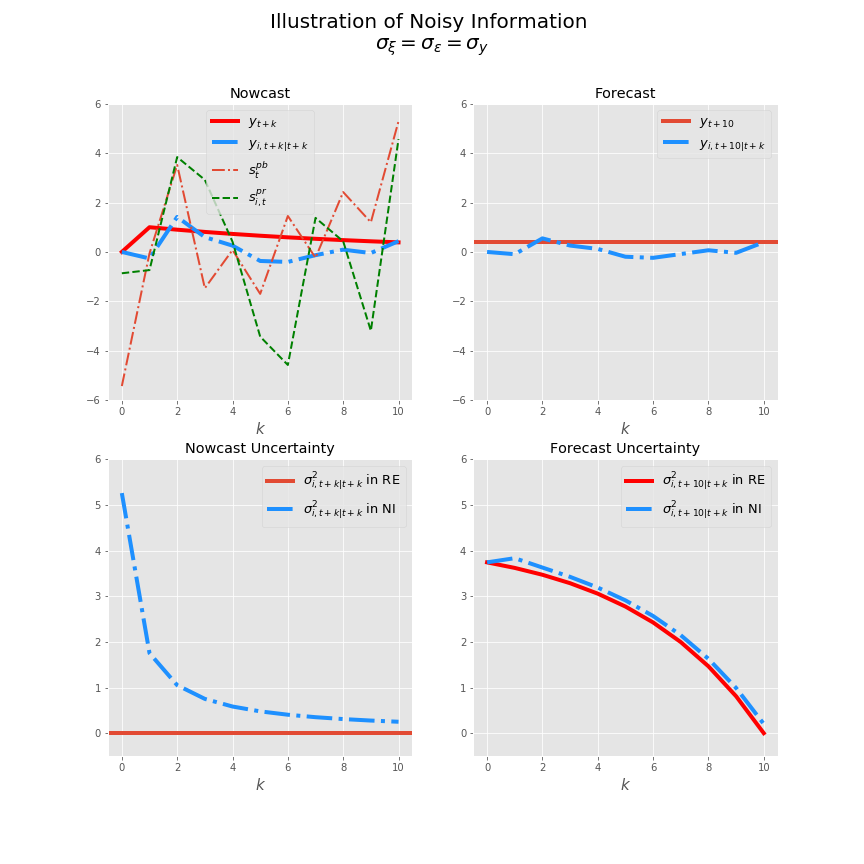
\includegraphics[width=13cm]{figures/ni_illustration.png}  
	\caption{Illustration Noisy Information}
\end{figure}


\subsubsection{Population moments}

\begin{eqnarray}
\begin{aligned}
\bar y_{t+h|t} & = \rho^h [(1-PH) \underbrace{\bar  y_{t+h|t-1}}_{\text{Average prior}} + P \underbrace{\bar s_{t}}_{\text{Average Signals}}] \\
& = (1-PH) \bar y_{t+h|t-1}+ P [\epsilon_t, 0]' \\
& = (1-PH) \bar y_{t+h|t-1} + P \epsilon_t
\end{aligned}
\end{eqnarray}

One of the major implications from NI models is that both individual forecast and ucnertainty behaves the same pattern as population forecasts. 

In parituclar, the same as indivdiual forecast erro, average forecast errors have serial correlation with the same auto regression parameter $\rho^h(1-PH)$. 

As to the uncertainty, as it does not depend on realized signals and the precision is the same aross all agents, average variance $\bar \Sigma_{t+h|t}$ is equal to the variance of each individual. 

Also, same as the individual variance, the variance unambiguiously drop in each vintage of revision. But since the signal is noisy, agents partially react to the news and uncertainty does not drop as efficiently as FIRE. 

\begin{eqnarray}
\bar \Sigma^2_{t+h|t} -  \bar \Sigma^2_{t+h|t-1}< 0 
\end{eqnarray}

NI also predicts non-zero disagreements in the presence of private signals. The behavior of disagreements across agents come from the difference in realized private signals. Specifically, it is equal to the following. 

\begin{eqnarray}
\begin{aligned}
\overline {Disg}_{t+h|t} = \rho^{2h} P^2_\xi \sigma^2_\xi  
\end{aligned}
\end{eqnarray}

First, the disagreements increase with the forecast horizon.  Second, the disagreements depends on noisiness private signals, but not on that of public signals and the variance of the true variable $y$. Third, similar to SE, the disagreements also increase with the rigidity parameter $P$ in this model.

The disagreements increase as time goes from $t-1$ to $t$. Also, as the time approaches $t+h$, the disagreements increase. This seems counterintuitive. But the reason is that here the disagreenments always exist simply because agents receive private signals, this disagreements is actually amplified as time goes forward. 


\subsubsection{Summary of predictions from noisy information}

$\bullet$  Invididual expectation adjusts in each period, but only partially adjusts to new information. \\
$\bullet$ Unlike sticky expectation, slugishness in adjustment or serial correlation of adjustment exists in individual level. The correlation parameter decreases with forecast horizon, which is not the case in sticky expectation.\\
$\bullet$  Individual variance unambiguously drops each period as one approaches the period of realization. In sticky expectation, it increases regardless of updating or not. \\ 
$\bullet$  Population average forecast partially adjusts to news and has serial correlation as the individual level. \\
$\bullet$  Population disagreements rise in each period as time approaches the period of realization. Disagreetments will never be zero. \\
$\bullet$  Average variance declines unambiguously each period. 

\subsection{Comparing FIRE, SE and NI}

Figure \ref{ir_pop} plots the impulse responses of population moments of forecasts accroding to different theories. As we focus on the dynamics of revision as one approaches the terminate date, i.e. forecast of $y_{t+h}$ at $t$, $t+1$, $t+2$ till $t+h$ instead of forecasts with fixed horizon, i.e. $y_{t+h}$,$y_{t+h+1}$. 

This is the most intuitively seen in the dynamics of uncertainty. In particular, as one appraoch the realization $t+h$, uncertainty necessarily drop for FIRE and attains zero at the last period.  

\begin{figure}[h]\label{ir_pop}
	\centering
	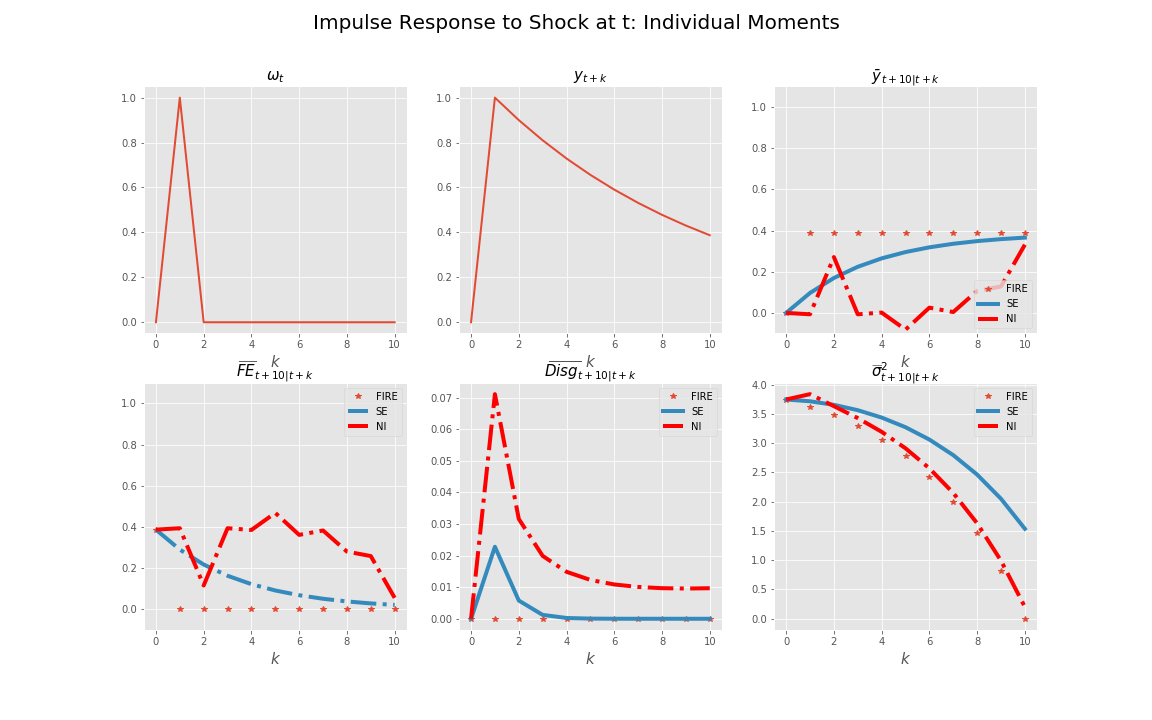
\includegraphics[width=14cm]{figures/ir_popseni.png} 
	\caption{Impulse responses of moments to a shock to inflation}
\end{figure}

One of the common predictions of SE and NI is there is information rigidity or stickiness of expecatations.  But both theory have suble difference in implied rigidity. I illustrate this in Figure \ref{rigidity}. One notable difference is that SE's rigidty is exogeously fixed. NI's rigidity is endogeously determined by the noisiness of the signals and it is time varying. 
 
\begin{figure}[h]\label{rigidity}
	\centering
	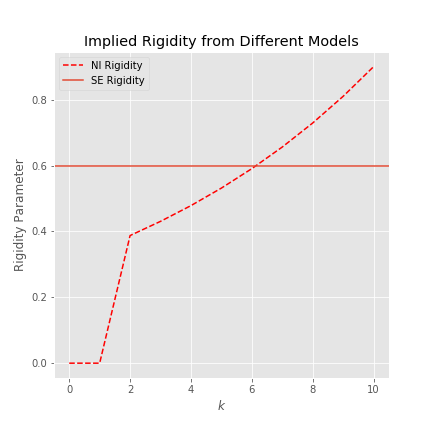
\includegraphics[width=13cm]{figures/rigidity.png} 
	\caption{Rigidity from Two Models}
\end{figure}


\subsection{Disucussion of other theories}

\begin{enumerate}
\item Rational inattention. 
\begin{itemize}
	\item Chris Sim's model.\cite{sims2003implications} Information serves the role of uncertainty reduction measured by relative entropy. Agents optimally trade off the fixed cost of being attentative versus the gain from uncertainty gain.   
	\item Ricardo Reis's model. \cite{reis2006inattentive}
	\item Xavier Gabaix's sparse matrix model. \cite{gabaix2014sparsity}
\end{itemize}

\item Epidemiologic view. \cite{carroll2003macroeconomic} Regardless of the microfoundations of the information rigidity, households infrequently get access to more rational-and-up-to-date expectations from professional forecasters with a poisson process. 


\item Strategic behaviors. Second order belief, i.e., what you believe of what others believe. \cite{angeletos2009incomplete}



\end{enumerate}

\section{Empirical Results}

\subsection{Data}


Professional Forecasters(SPF) and New York Fed Survey of Consumer Expectation(SCE). 

The structure of SPF allows us to directly test efficiency in revision as for the surveyees are asked to provide both currenct year forecast and 1-year-ahead inflation foreacst each quarter. 

SCE data, although each individual is surveyed for 12 months in a row, is only asked to forecast 1-year-ahead inflation. This is especially so in the density forecast. So we can only perform a weak test. 

We follow \cite{Manski} to estiamte the density distribution of each individual surveyee for SPF. New York Fed has followed the same procedures for SCE and directly provided their estimate of uncertainty. Therefore, I directly use them. 

We drop the outliers of uncertainty estimates at both top and bottom one percentiles as these are typically abnormals that are due to measurement errors or other reasons.   


A summary of the data information is as below. 

\begin{table}[]
			\caption{Information of Data}
	\begin{tabular}{lll}

		\hline 
		& SCE & SPF        \\
		\hline 
		Time period                                    & 2013-present                            & 2007-present             \\
		Frequency                                      & Monthly                                 & Quarterly                \\
		Sample Size                                    & 1,300                                   & 30-50                    \\
		Aggregate Var in Density                       & 1-yr  and 3-yr ahead inflation          & 1-yr CPI and PCE         \\
		Individual Var in Density                      & 1-yr earning growth                     & No                       \\
		Pannel Structure                               & stay up to 12 months                    & average stay for 5 years \\
		Demographic Info                        & Education, Income, Age, Location        & Industry    \\
		\hline 
	\end{tabular}
\end{table}


\subsection{Stylized Facts}

\subsubsection{Different Moments}

Figure \ref{UnceratitnyOtherMoments} plots the population uncertainty asgainst forecast errors and disagreements. 


The left  three figures look into the relationship between forecast error and uncertainty. In general, one may expect that  greater ex ante uncertainty implies greater ex post forecast errors. 

Many literature use disagreements and uncertainty interchangably but they are different objects. From the graph, we can also see in general uncertainty captures different information from disagreements. This is more so in professional forecaster data. There is a more obvious correlation between disgreements and uncertainty. 


Once implication from FIRE is that all individuals not only agree on mean but also share same degree of uncertainty. While in fact, we observe long-lasting heterogeneity in uncertainty both from professional forecasters and households. Figure \ref{IQR_Unceratitny} show that there is  not only dispersion of individual forecasts i.e. disagreements, but alslo notable heterogeneity in uncertainty. One stylized fact from these observations is that  the dispersion in ucnertainty seems persistent over time.  
 

Another prediction from FIRE is that there is unambigous uncertainty reduction as one appraoches to the date of realization. Figure \ref{RevisionHist} plots the average revision in mean forecasts and uncertainty. The the more negative the revision lies in, the more rational of the forecast.  


\begin{figure}[h]\label{UnceratitnyOtherMoments}
	\centering
	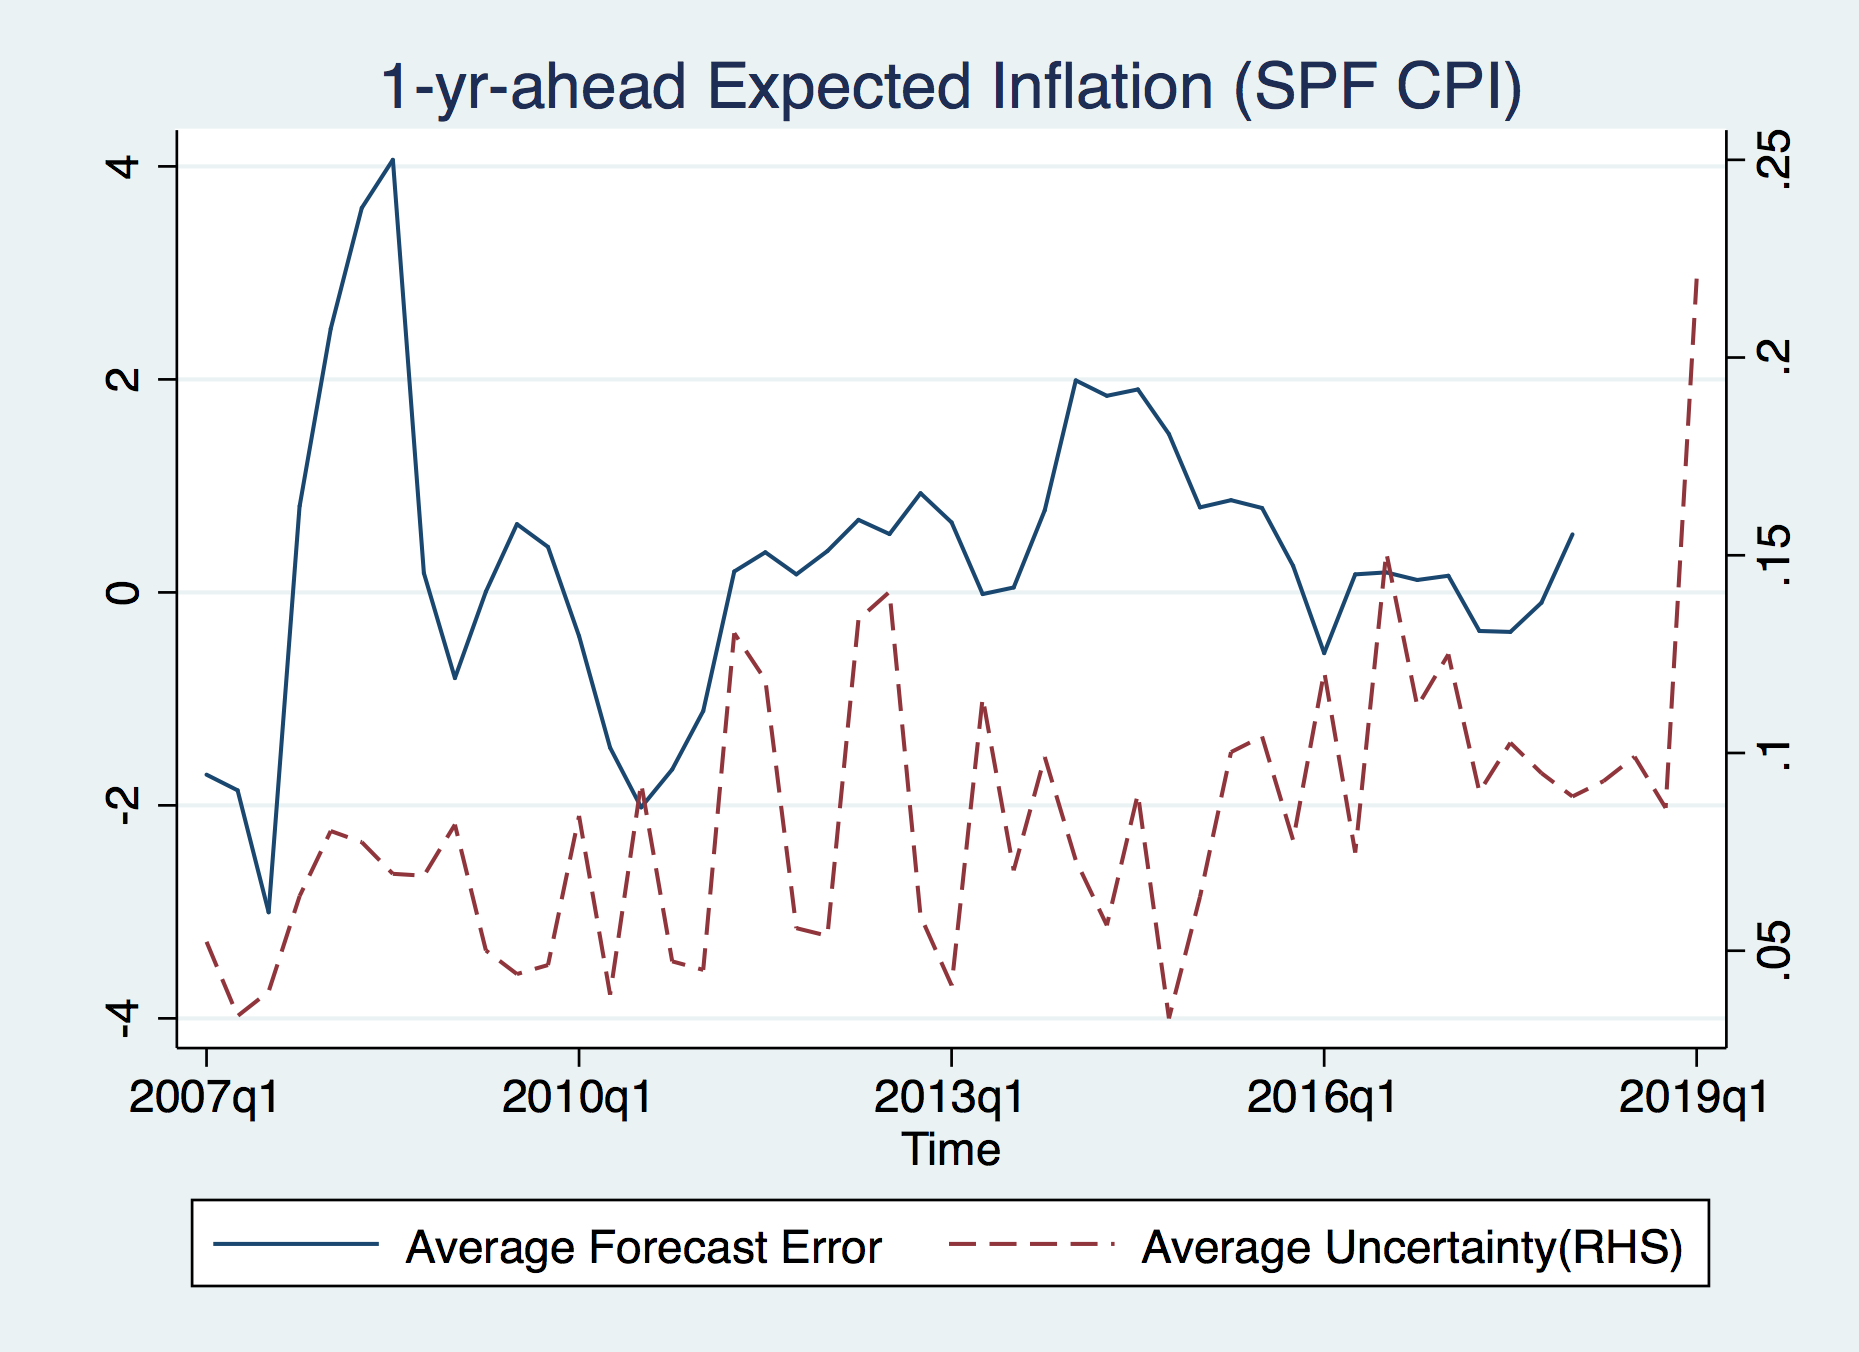
\includegraphics[width=6cm]{figures/fe_var2Q.png}
	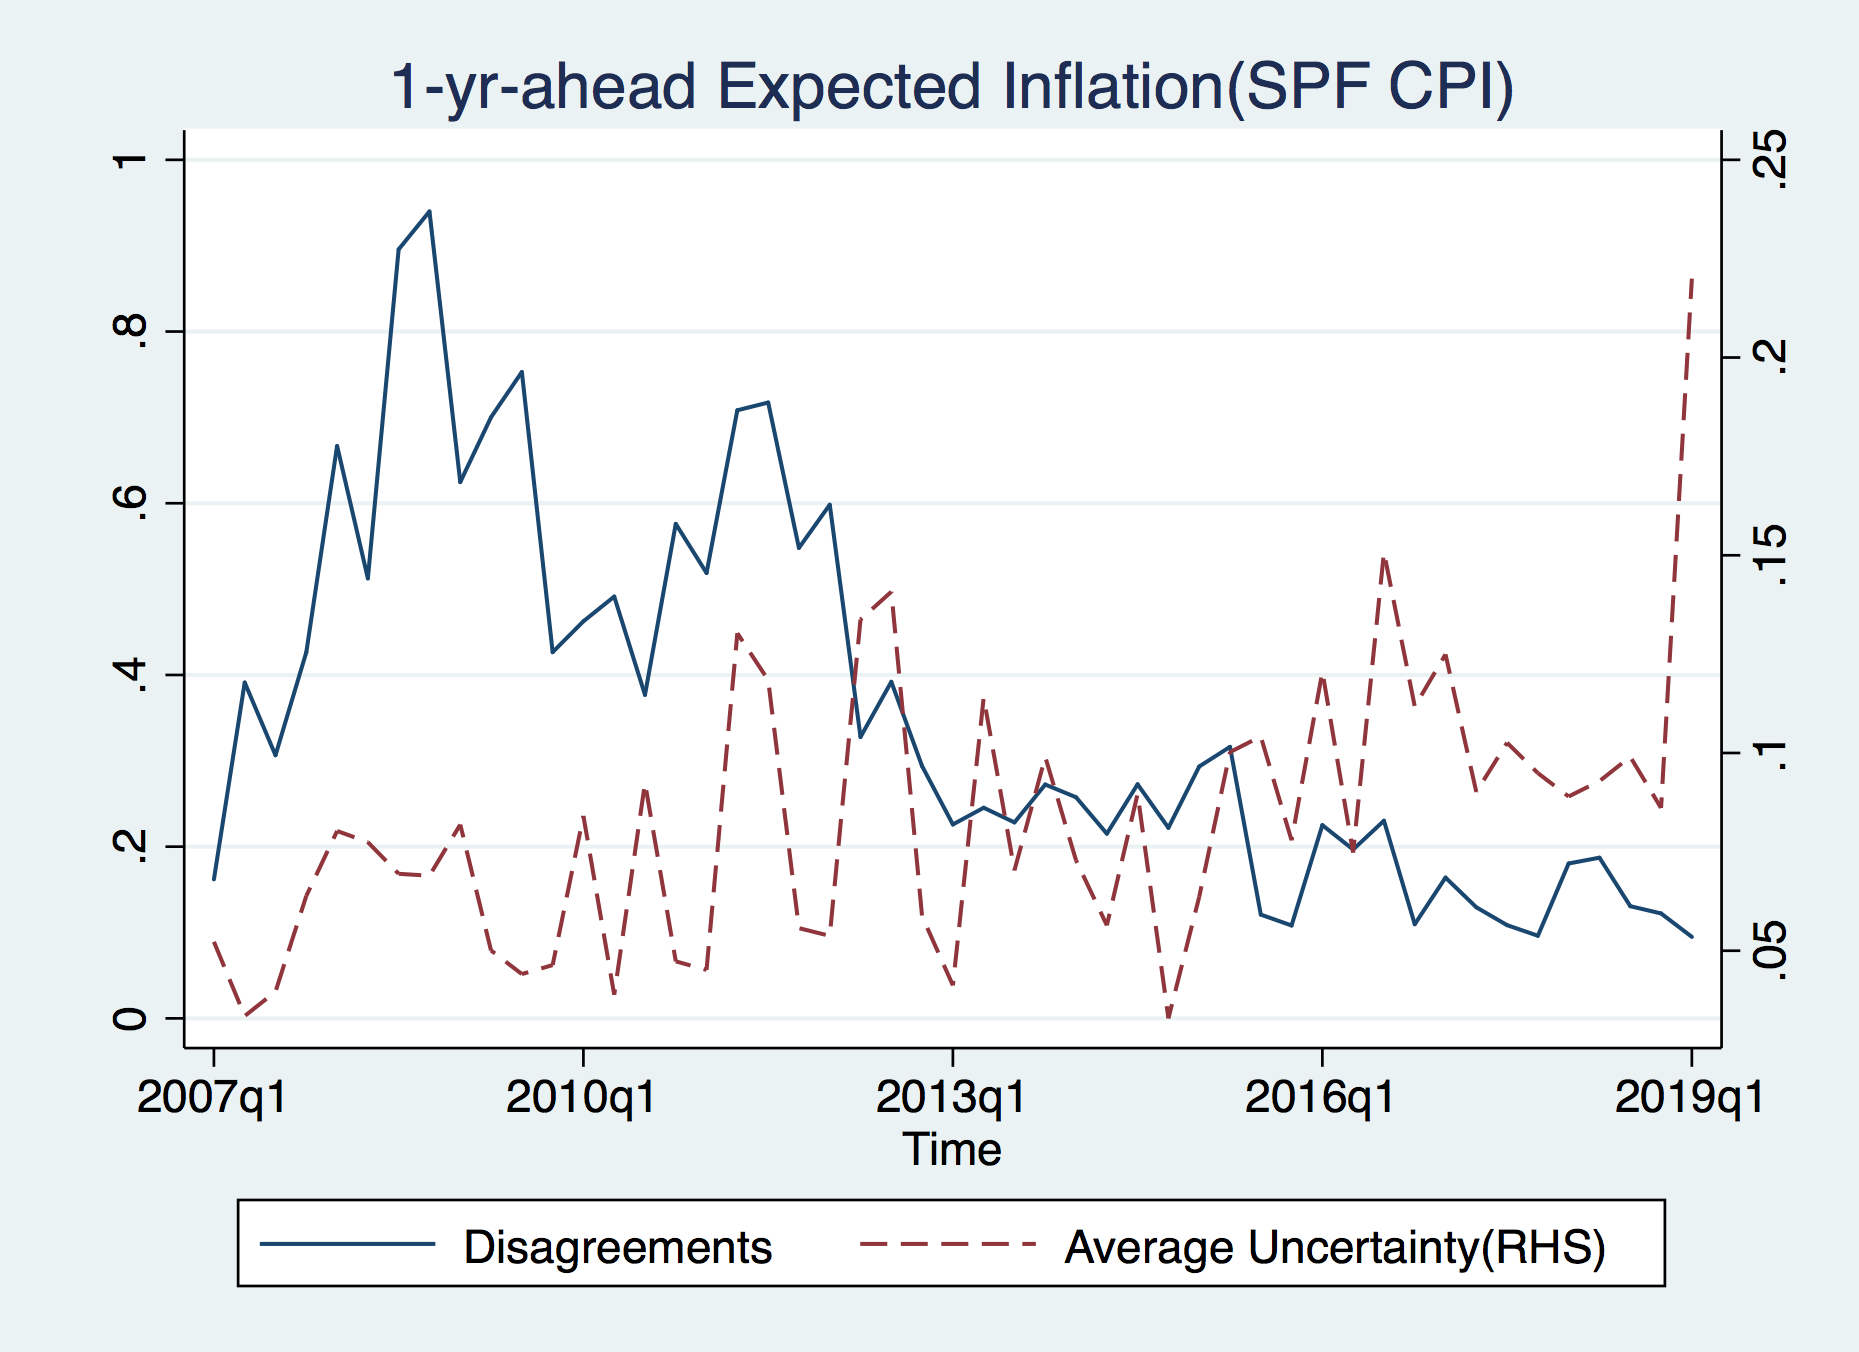
\includegraphics[width=6cm]{figures/var_disg2Q.png}\\
	\smallskip
	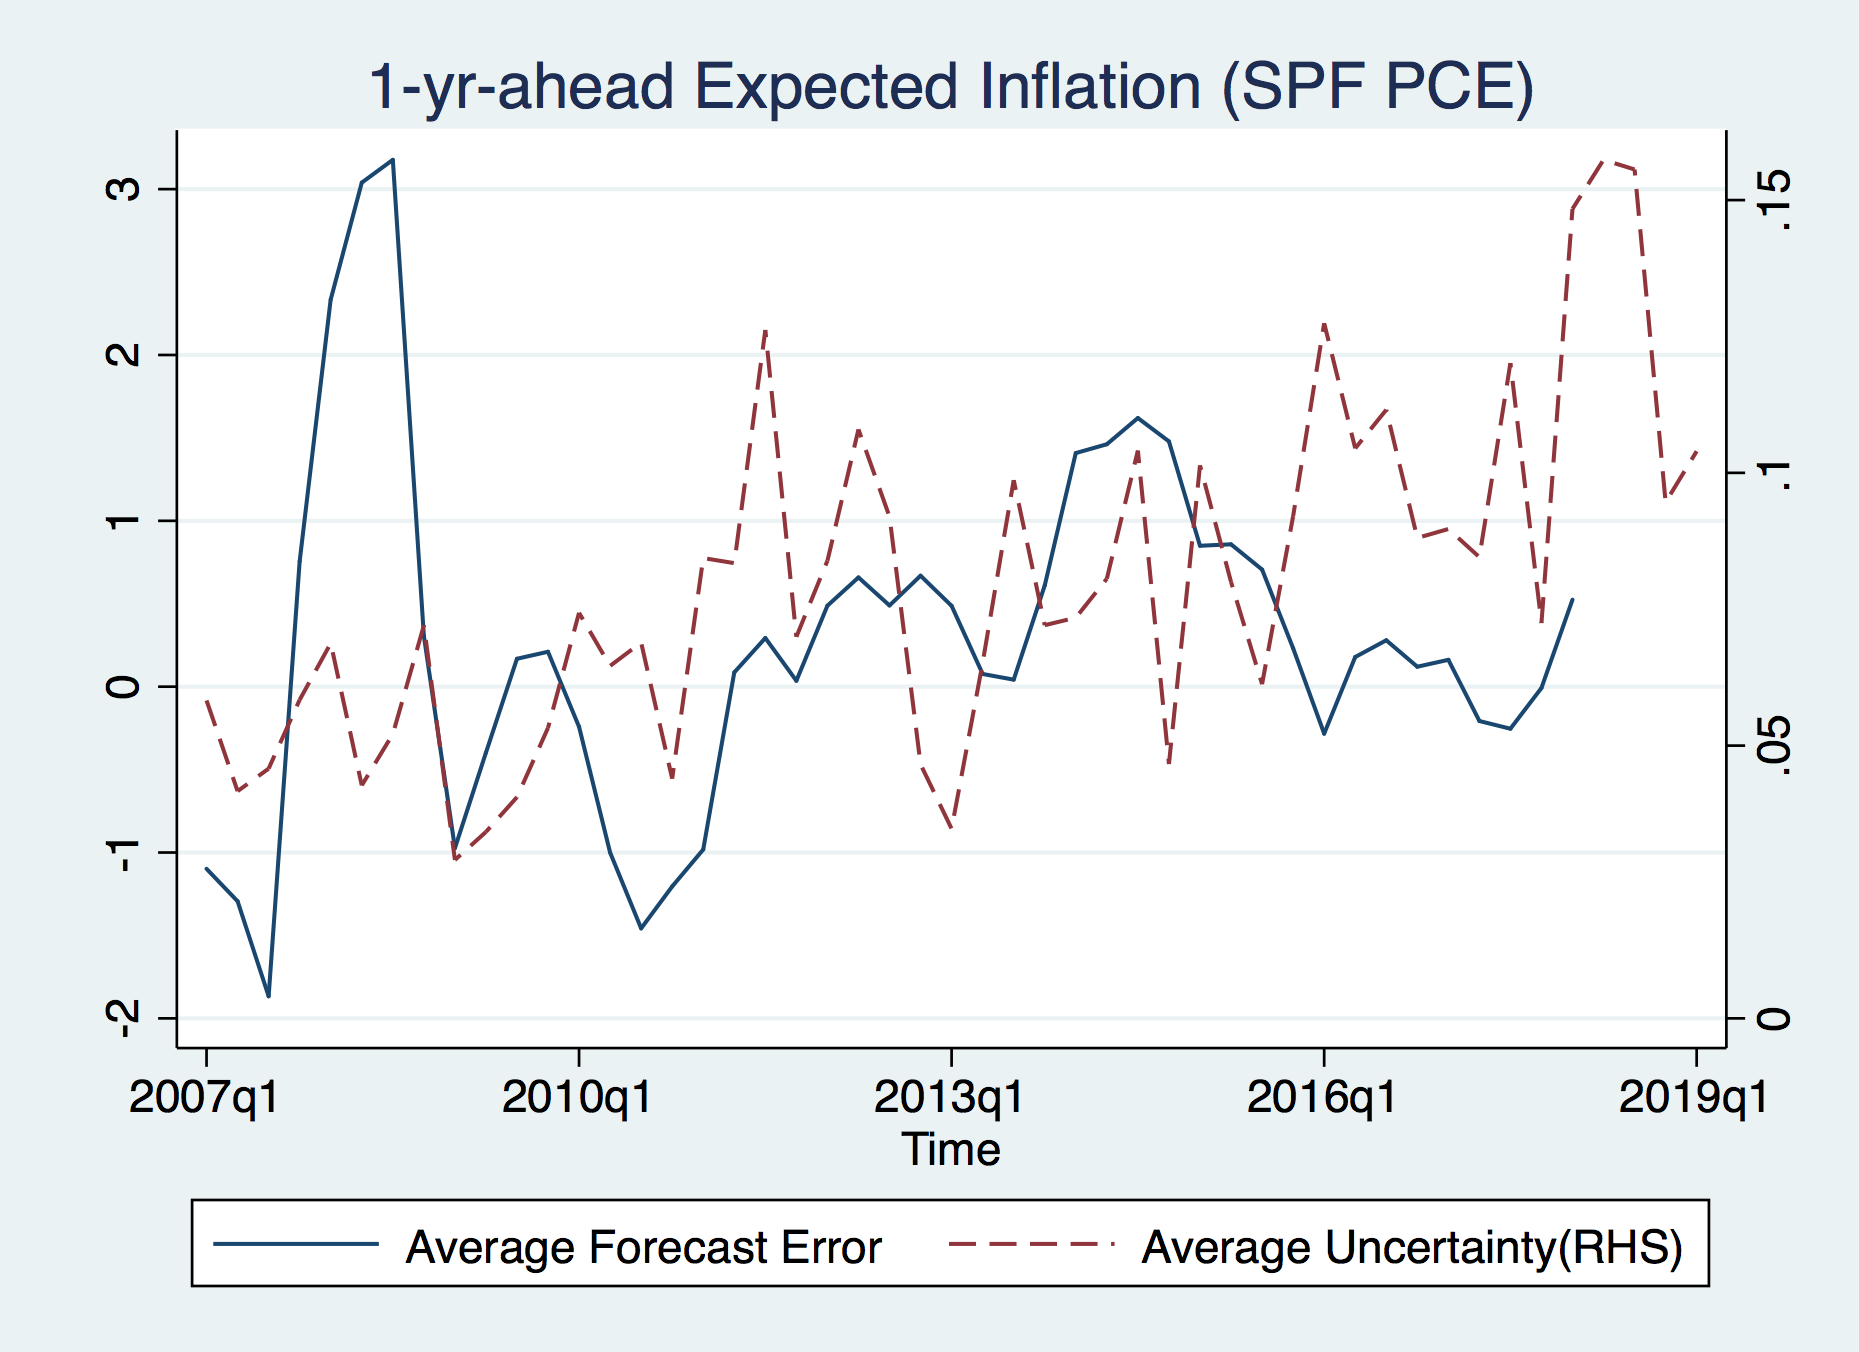
\includegraphics[width=6cm]{figures/fe_var3Q.png}
	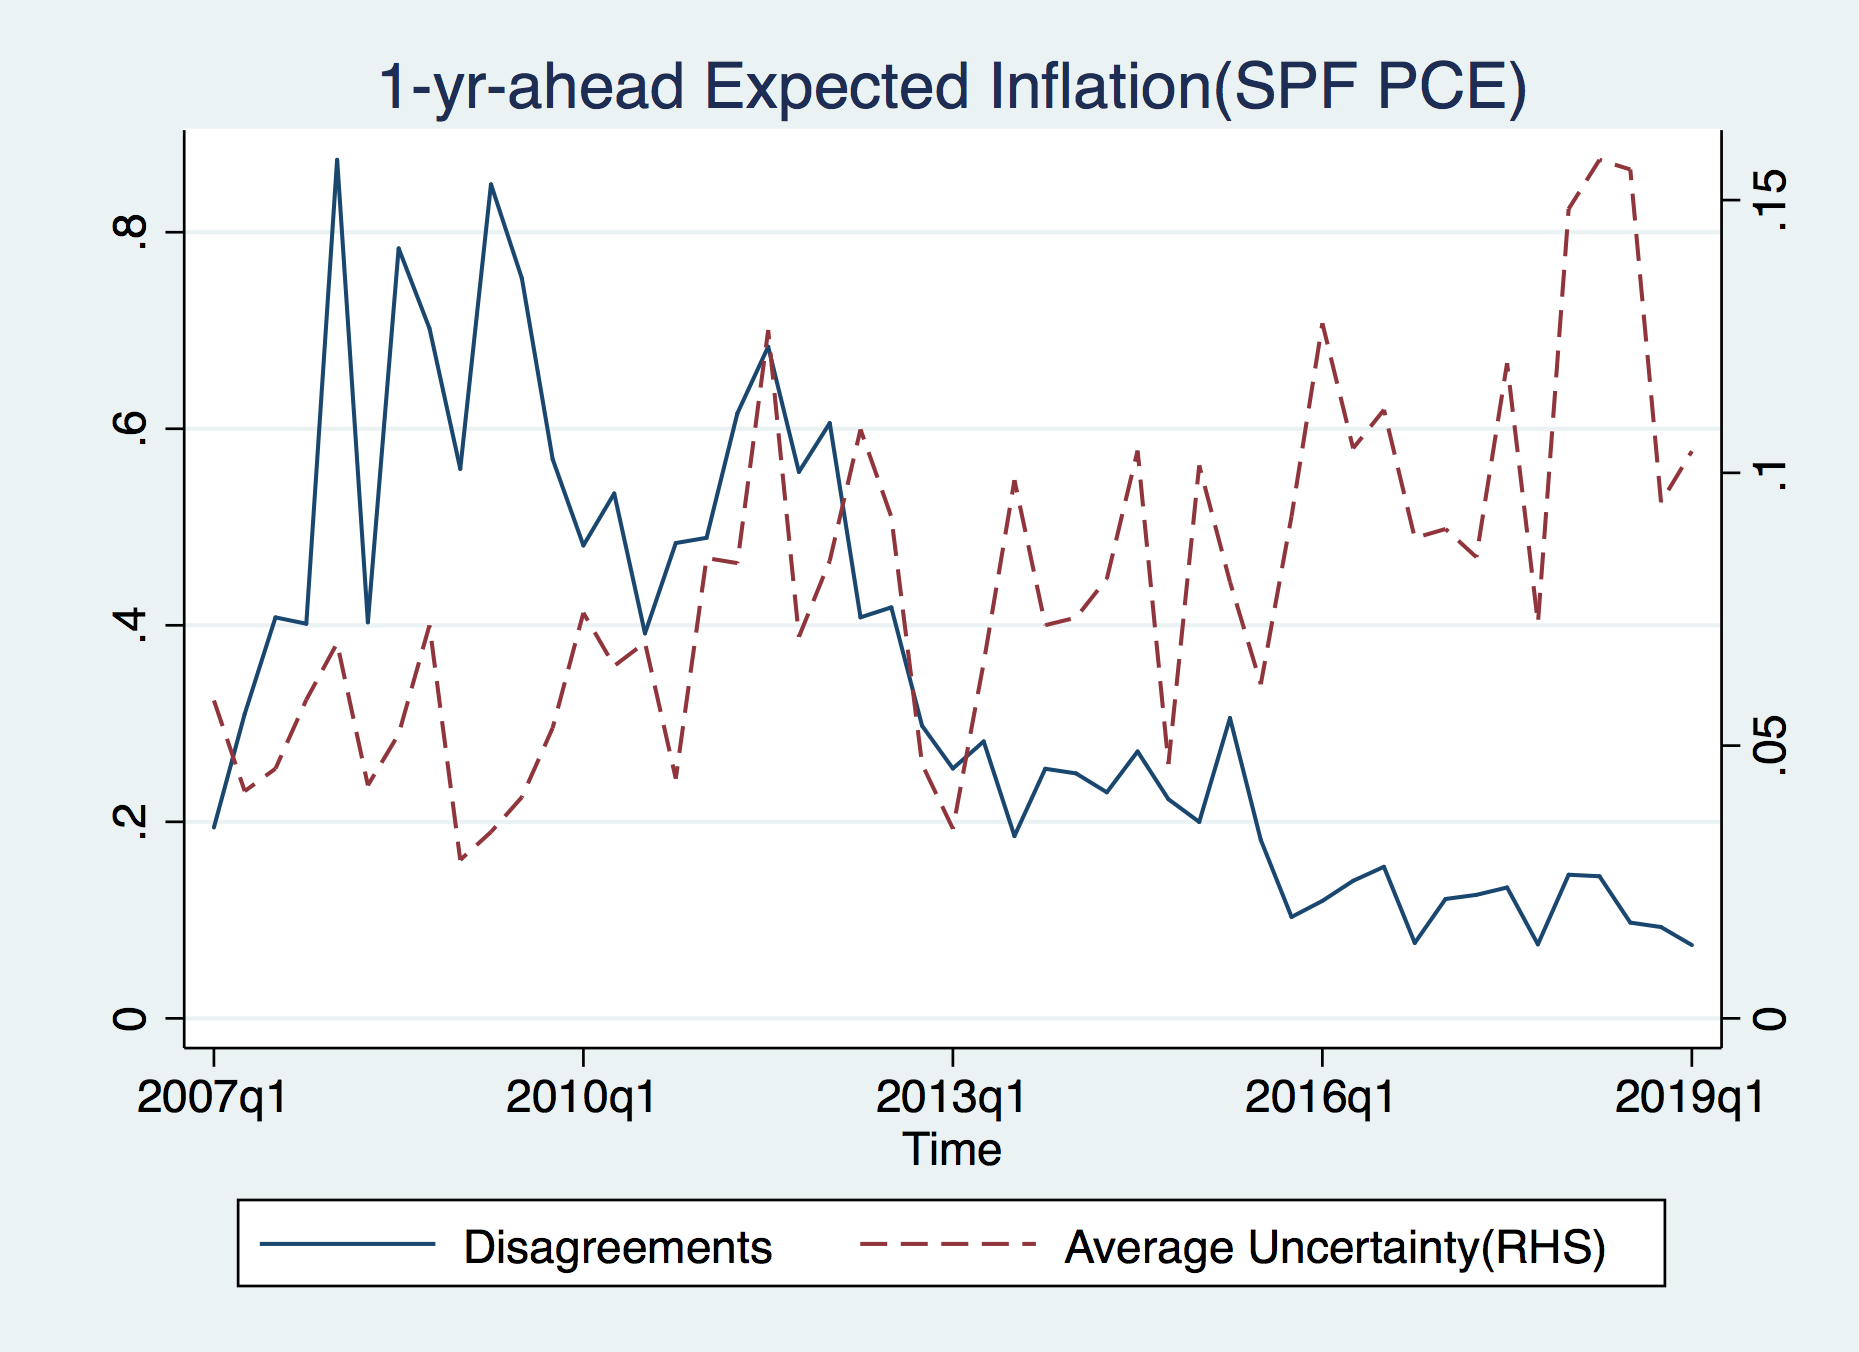
\includegraphics[width=6cm]{figures/var_disg3Q.png}\\
	\smallskip	
	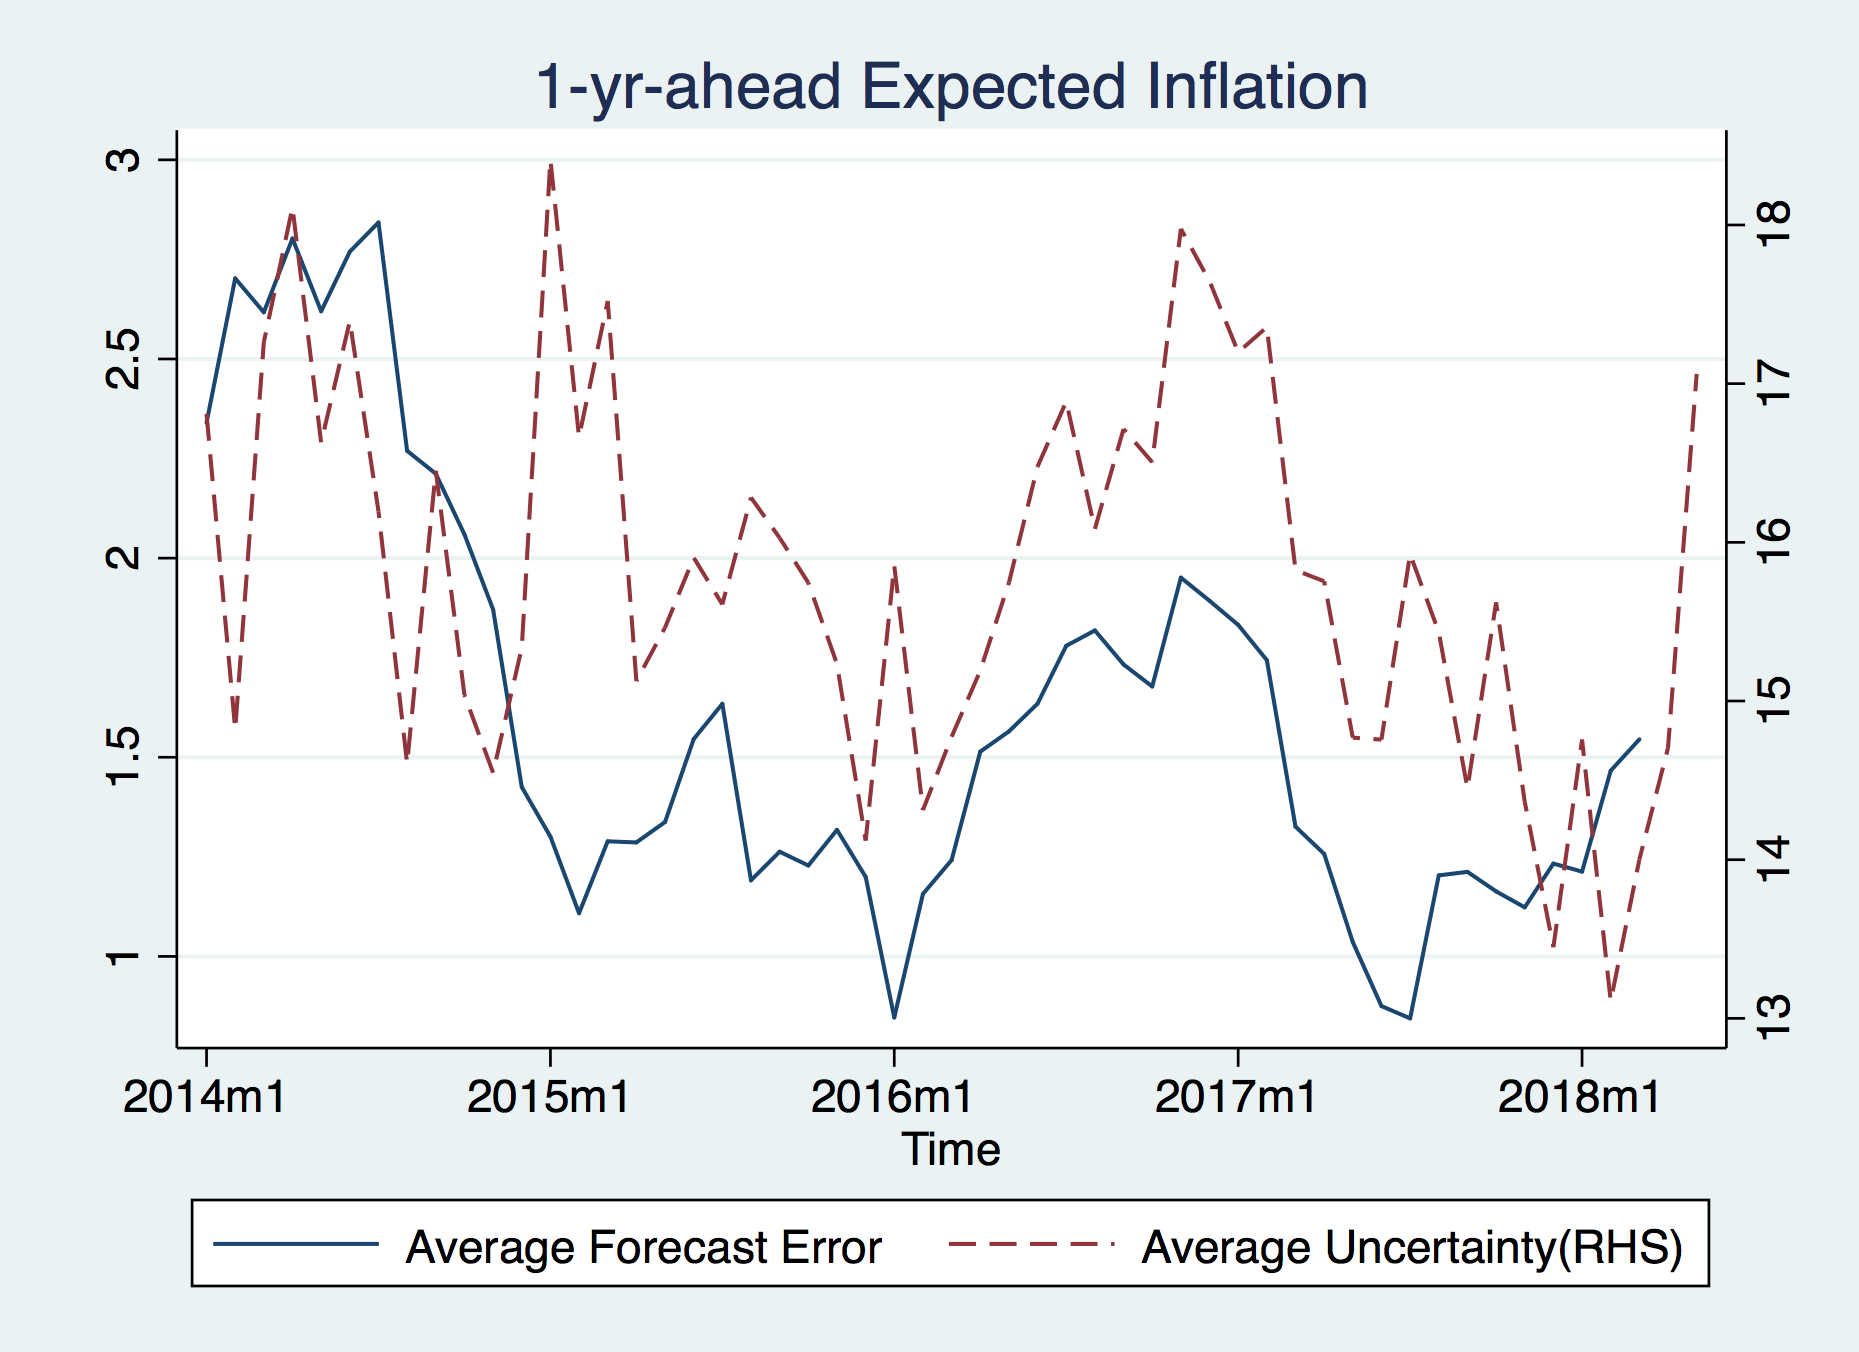
\includegraphics[width=6cm]{figures/fe_var.png}
	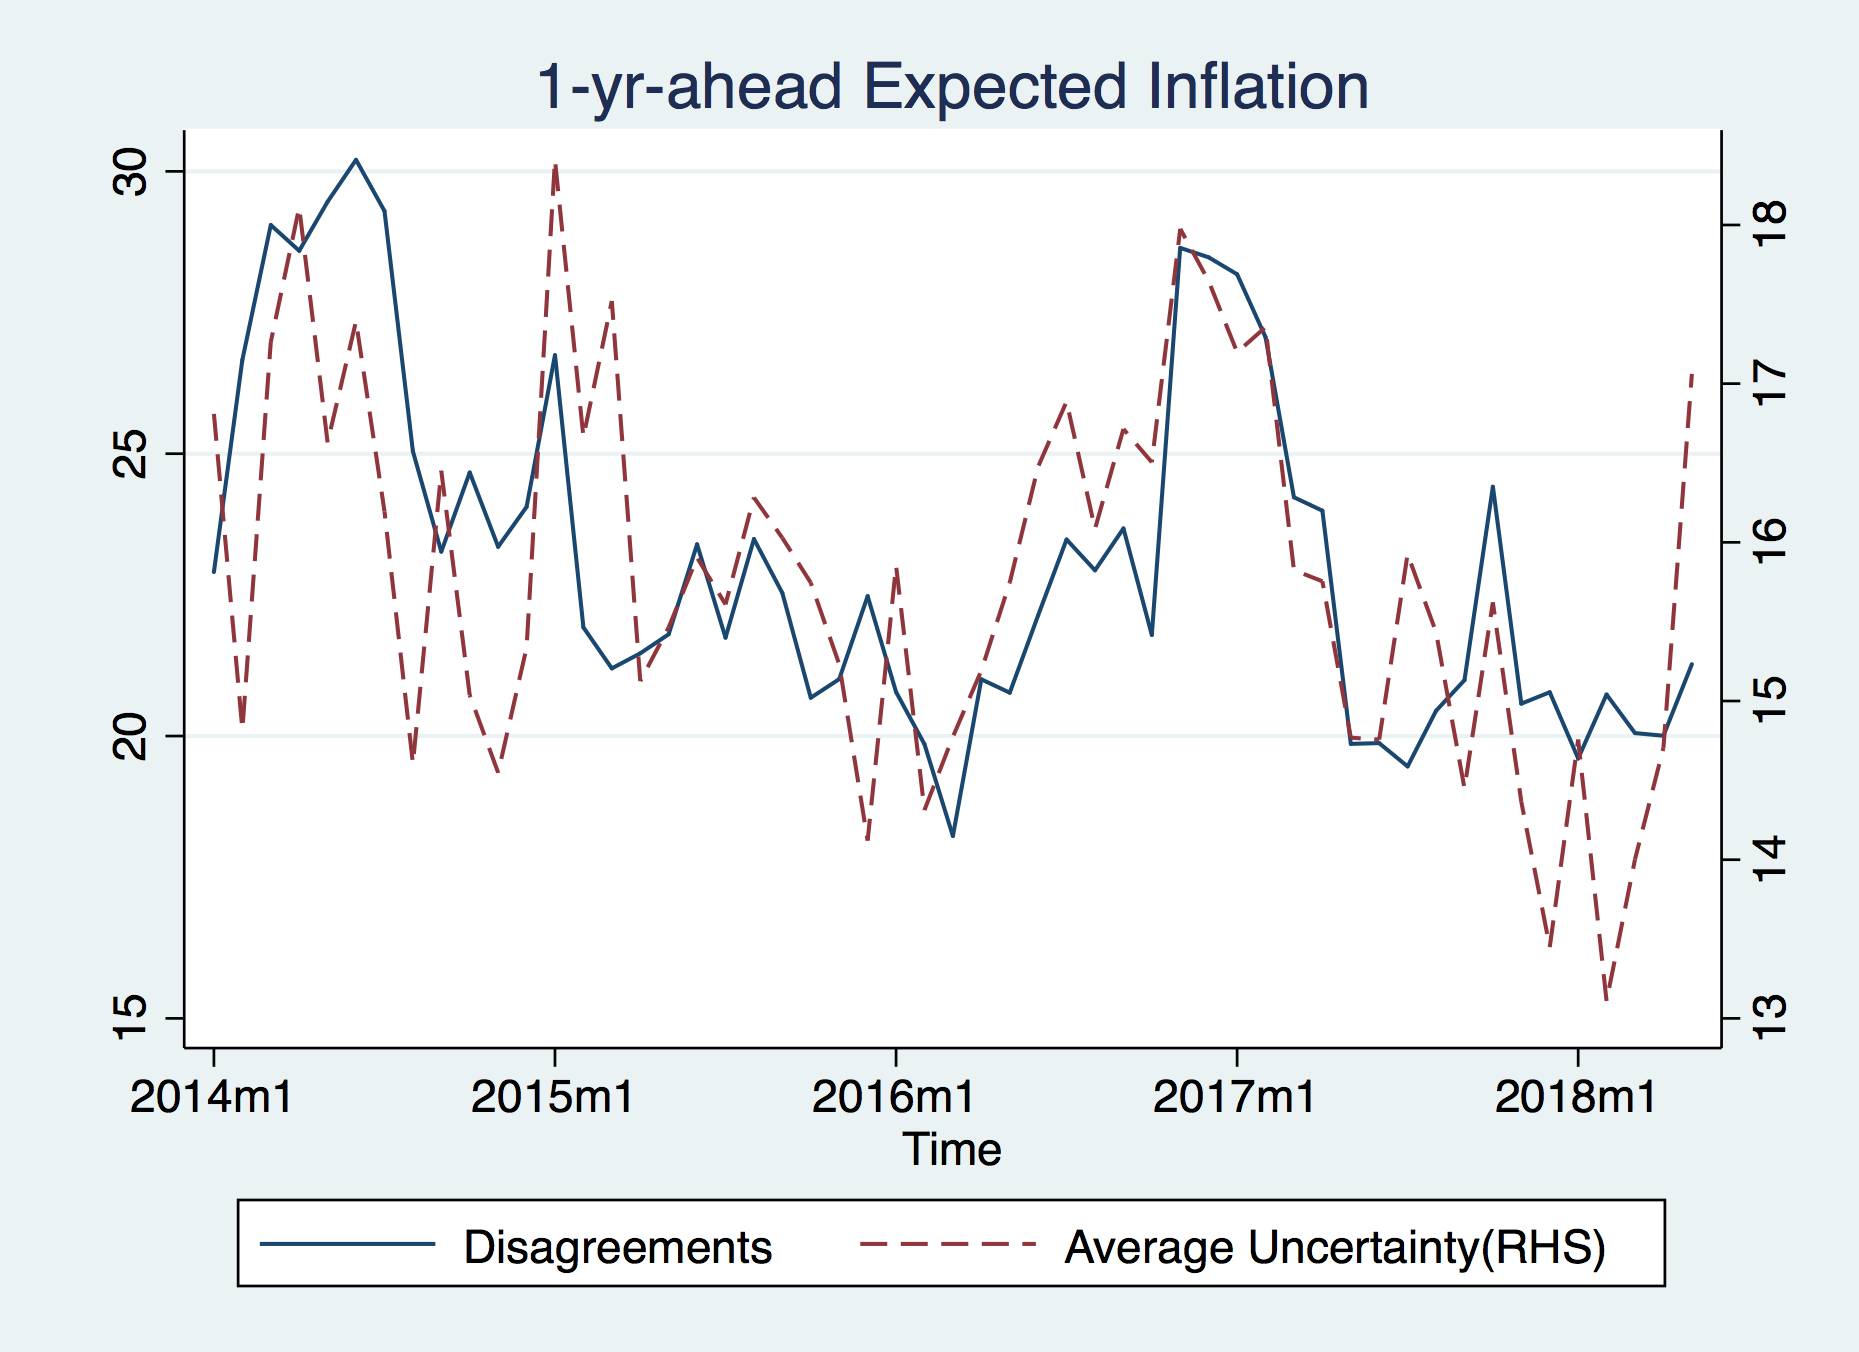
\includegraphics[width=6cm]{figures/var_disg.png}\\
		\caption{Unceratinty and Other Moments}
\end{figure}


\begin{figure}[h]\label{IQR_Unceratitny}
	\centering
	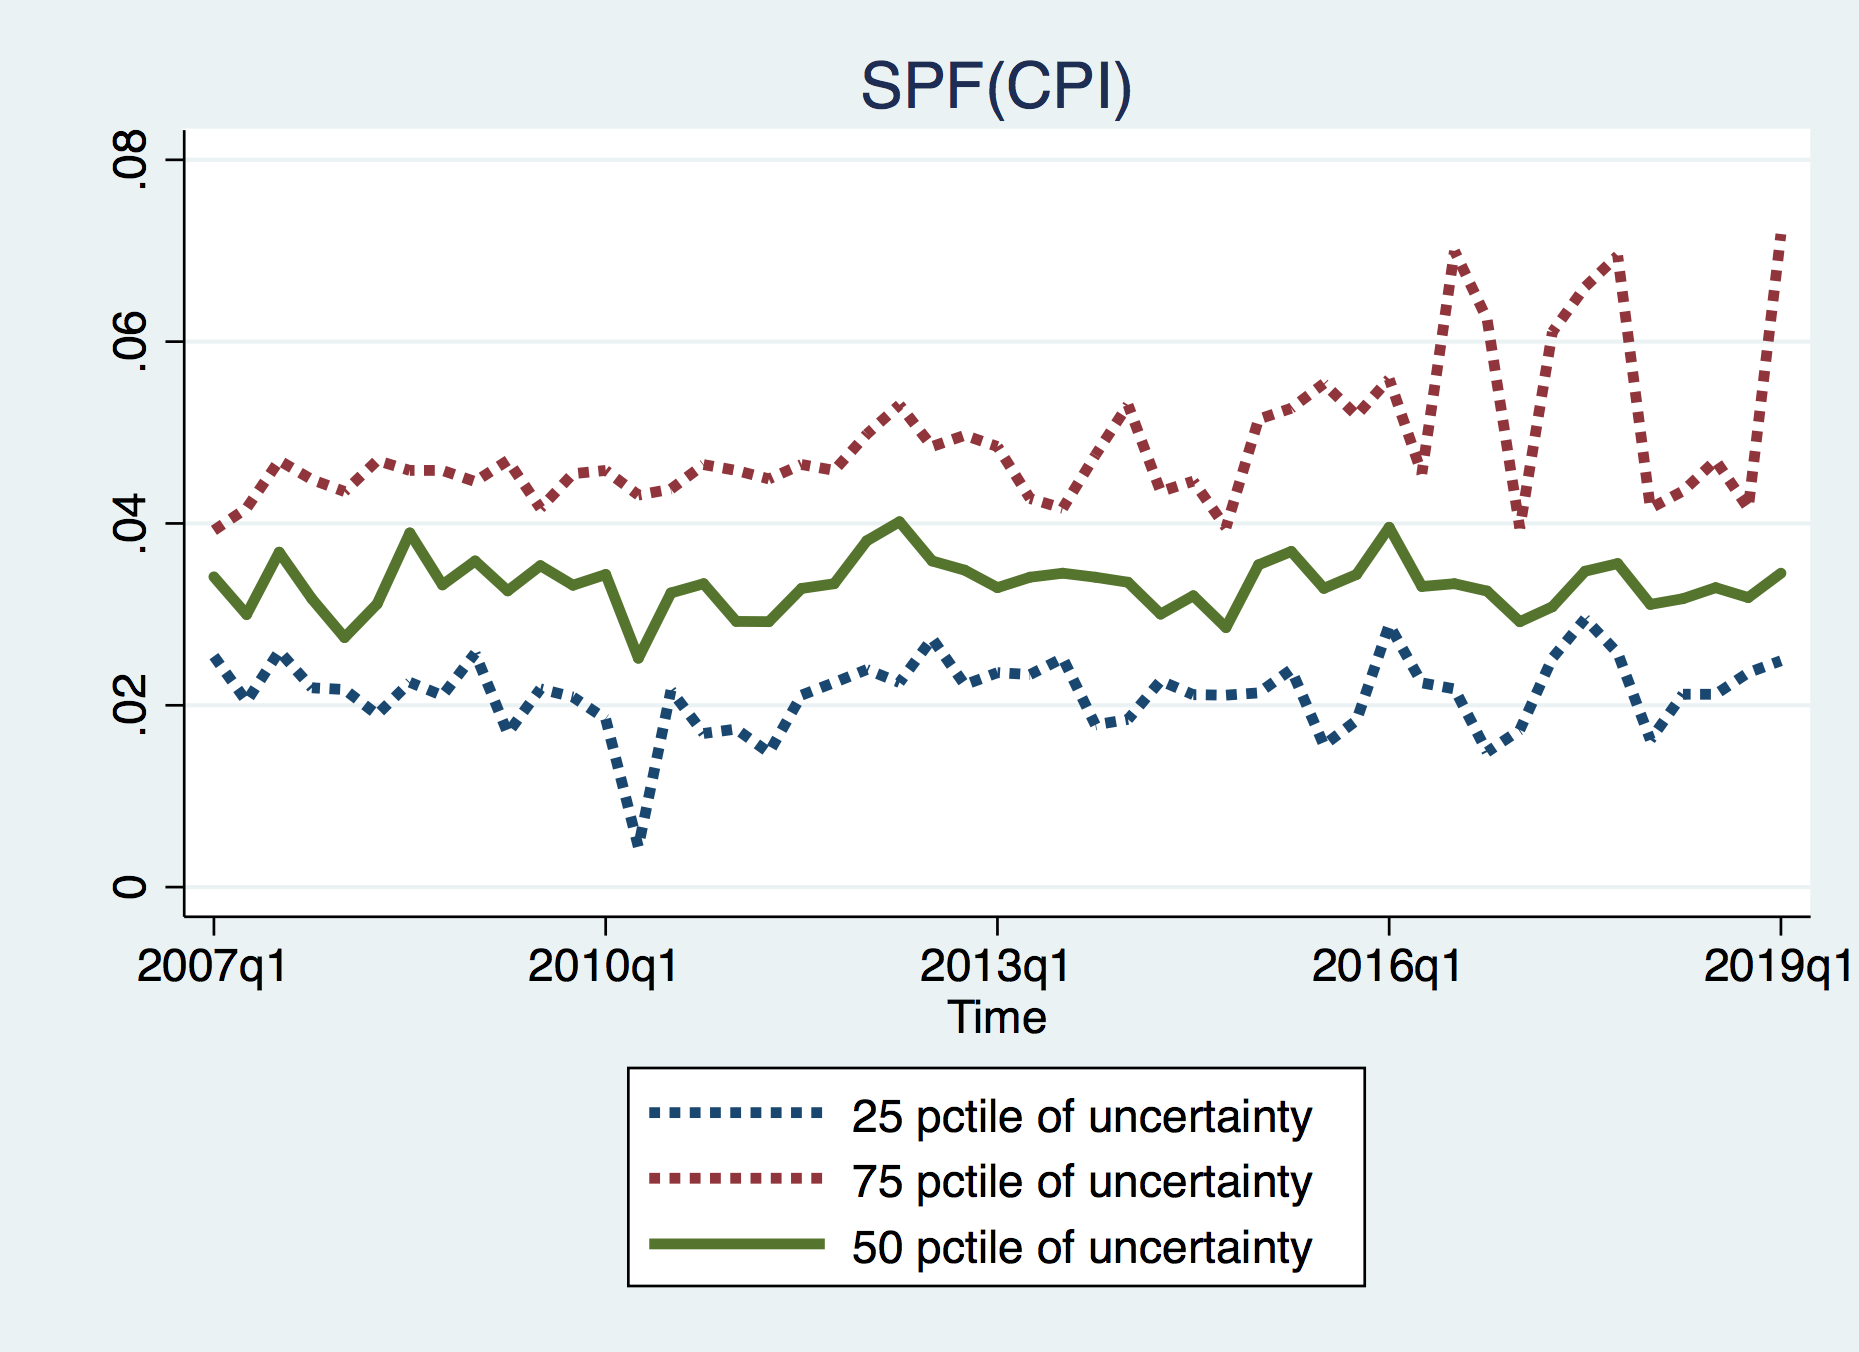
\includegraphics[width=8cm]{figures/IQRvarCPIQ.png} \\
	\smallskip
	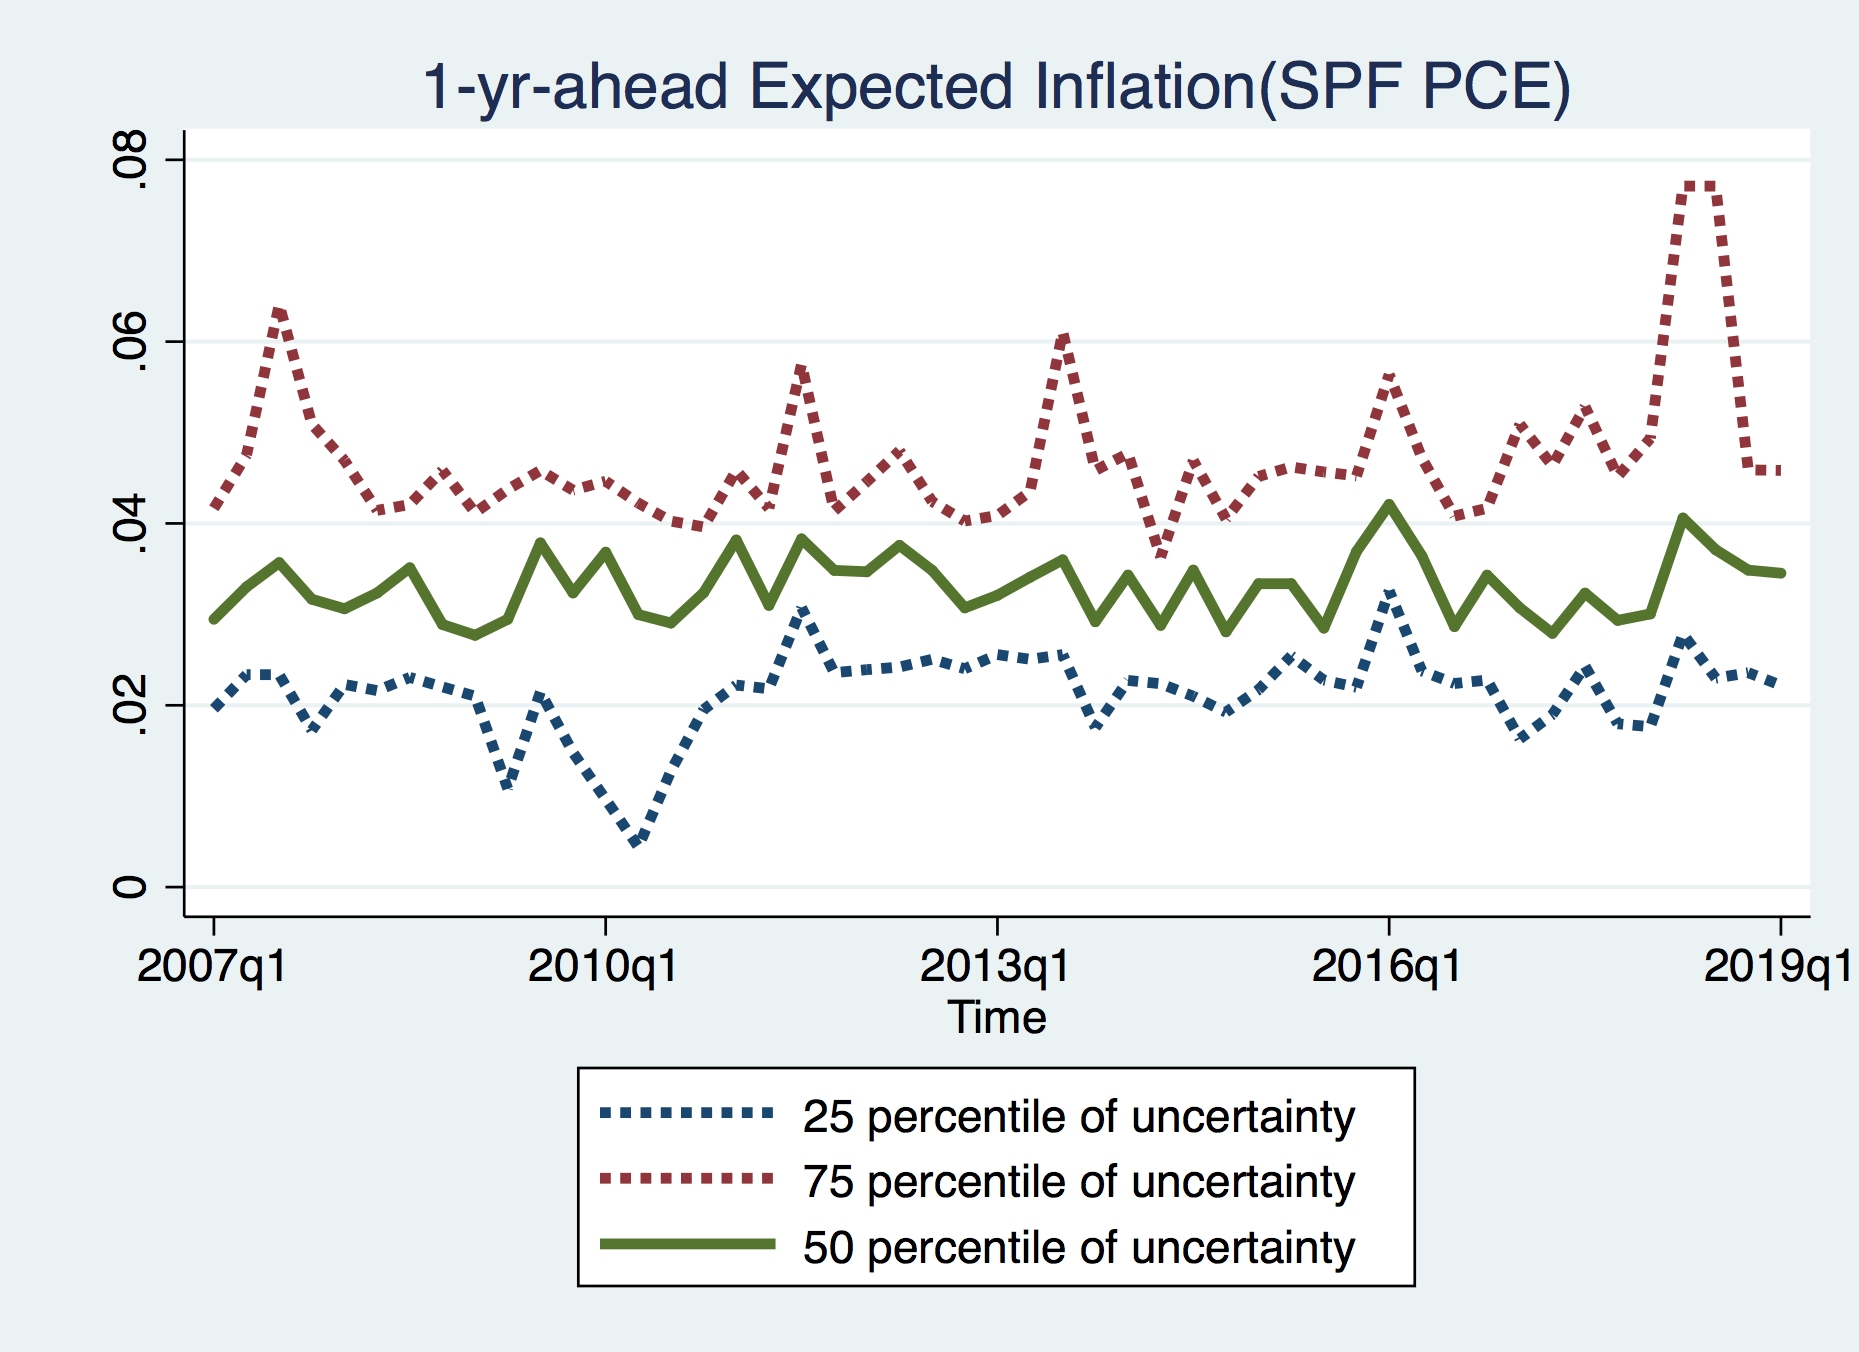
\includegraphics[width=8cm]{figures/IQRvarPCEQ.png}\\
		\smallskip
	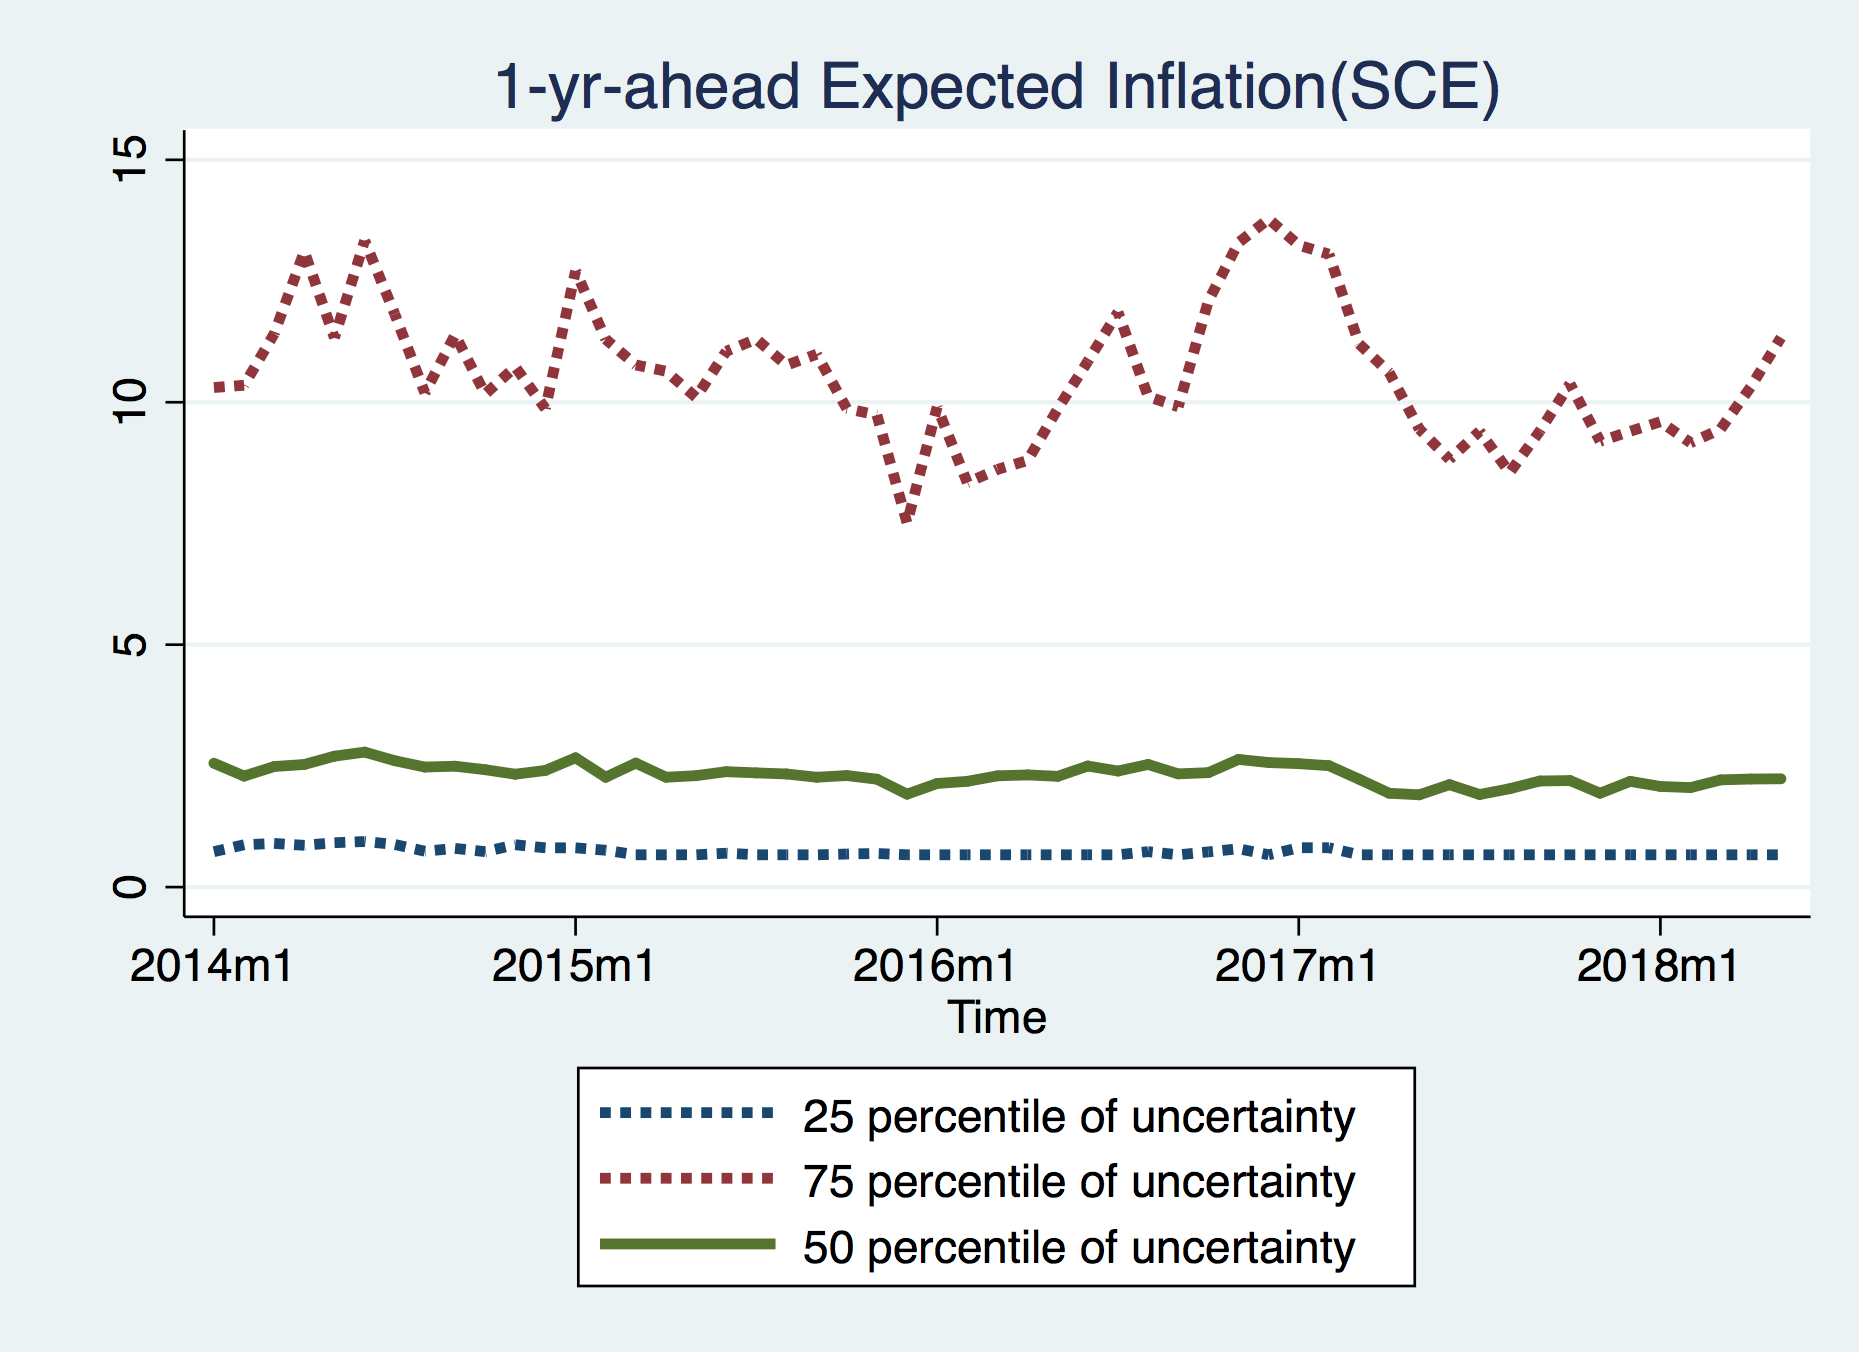
\includegraphics[width=8cm]{figures/IQRvarSCEM.png}\\
	\caption{Dispersion in Mean Forecast and Unceratinty }
\end{figure}


\begin{figure}[h]\label{Unceratitny_Histogram}
	\centering
	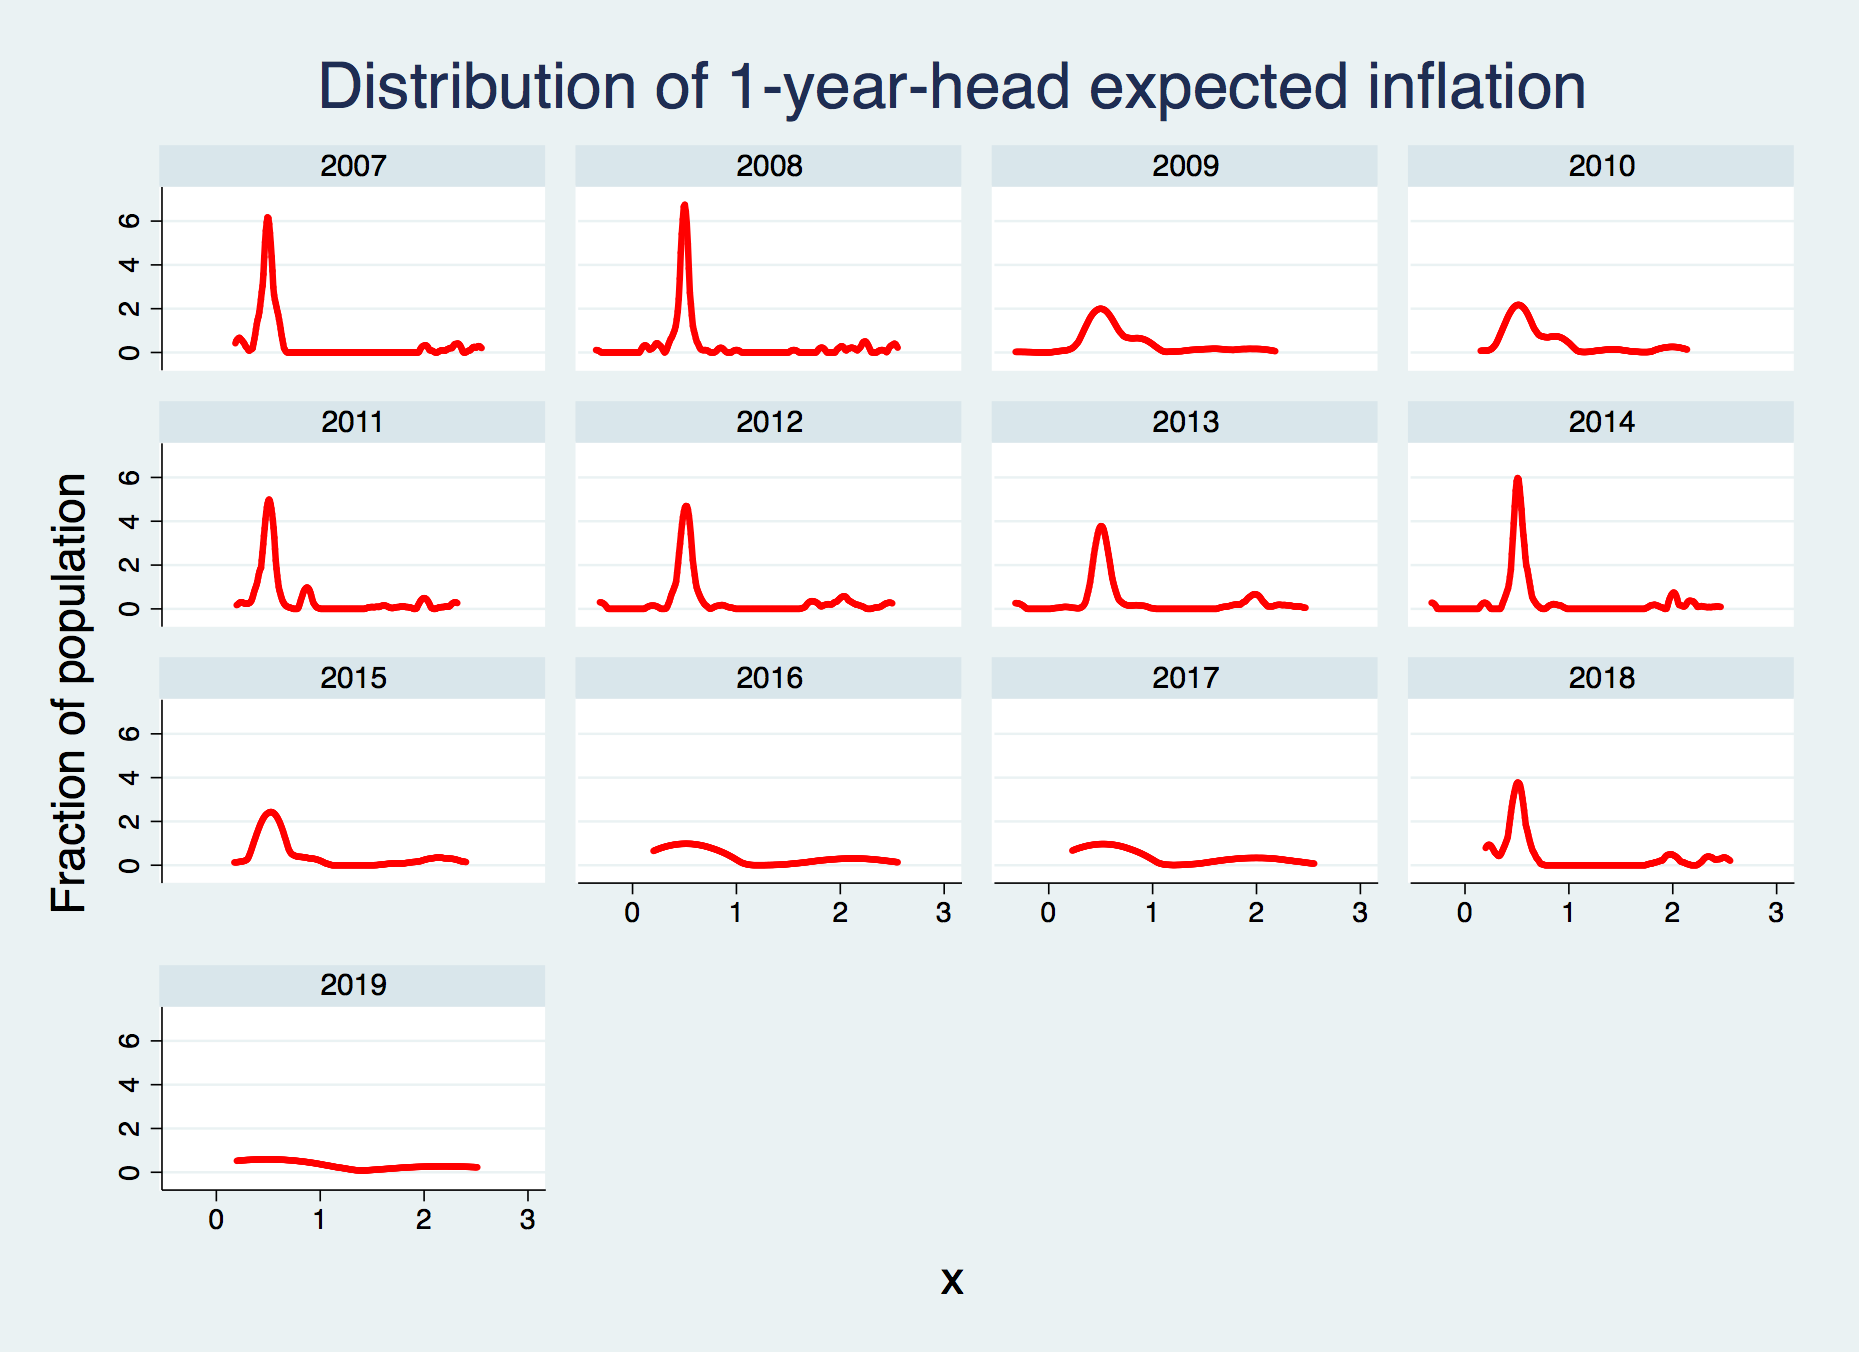
\includegraphics[width=6cm]{figures/PRCCPIMean1_hist.png} 
	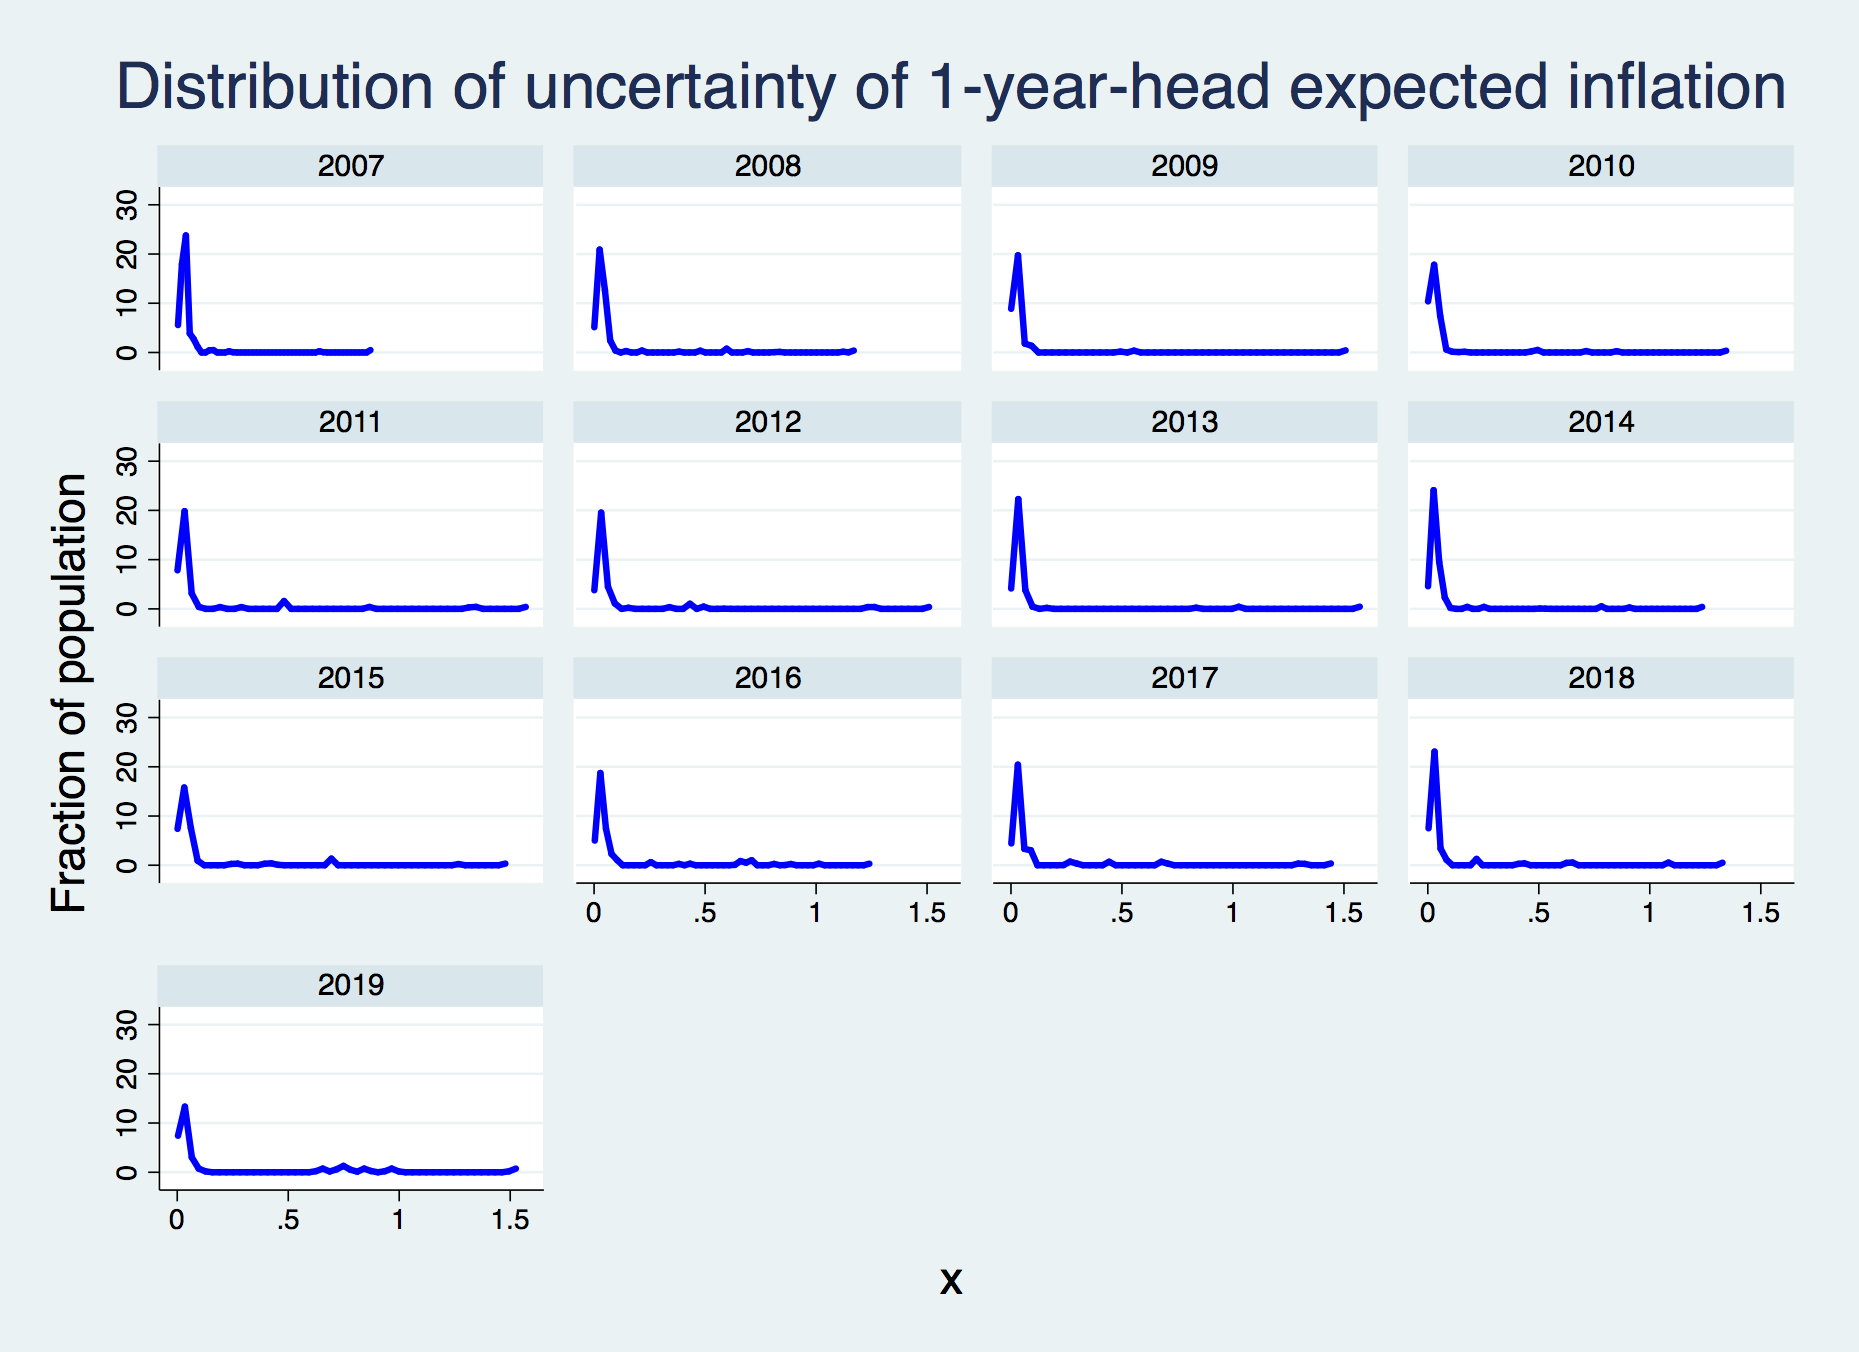
\includegraphics[width=6cm]{figures/PRCCPIVar1_hist.png}  \\
	\smallskip
		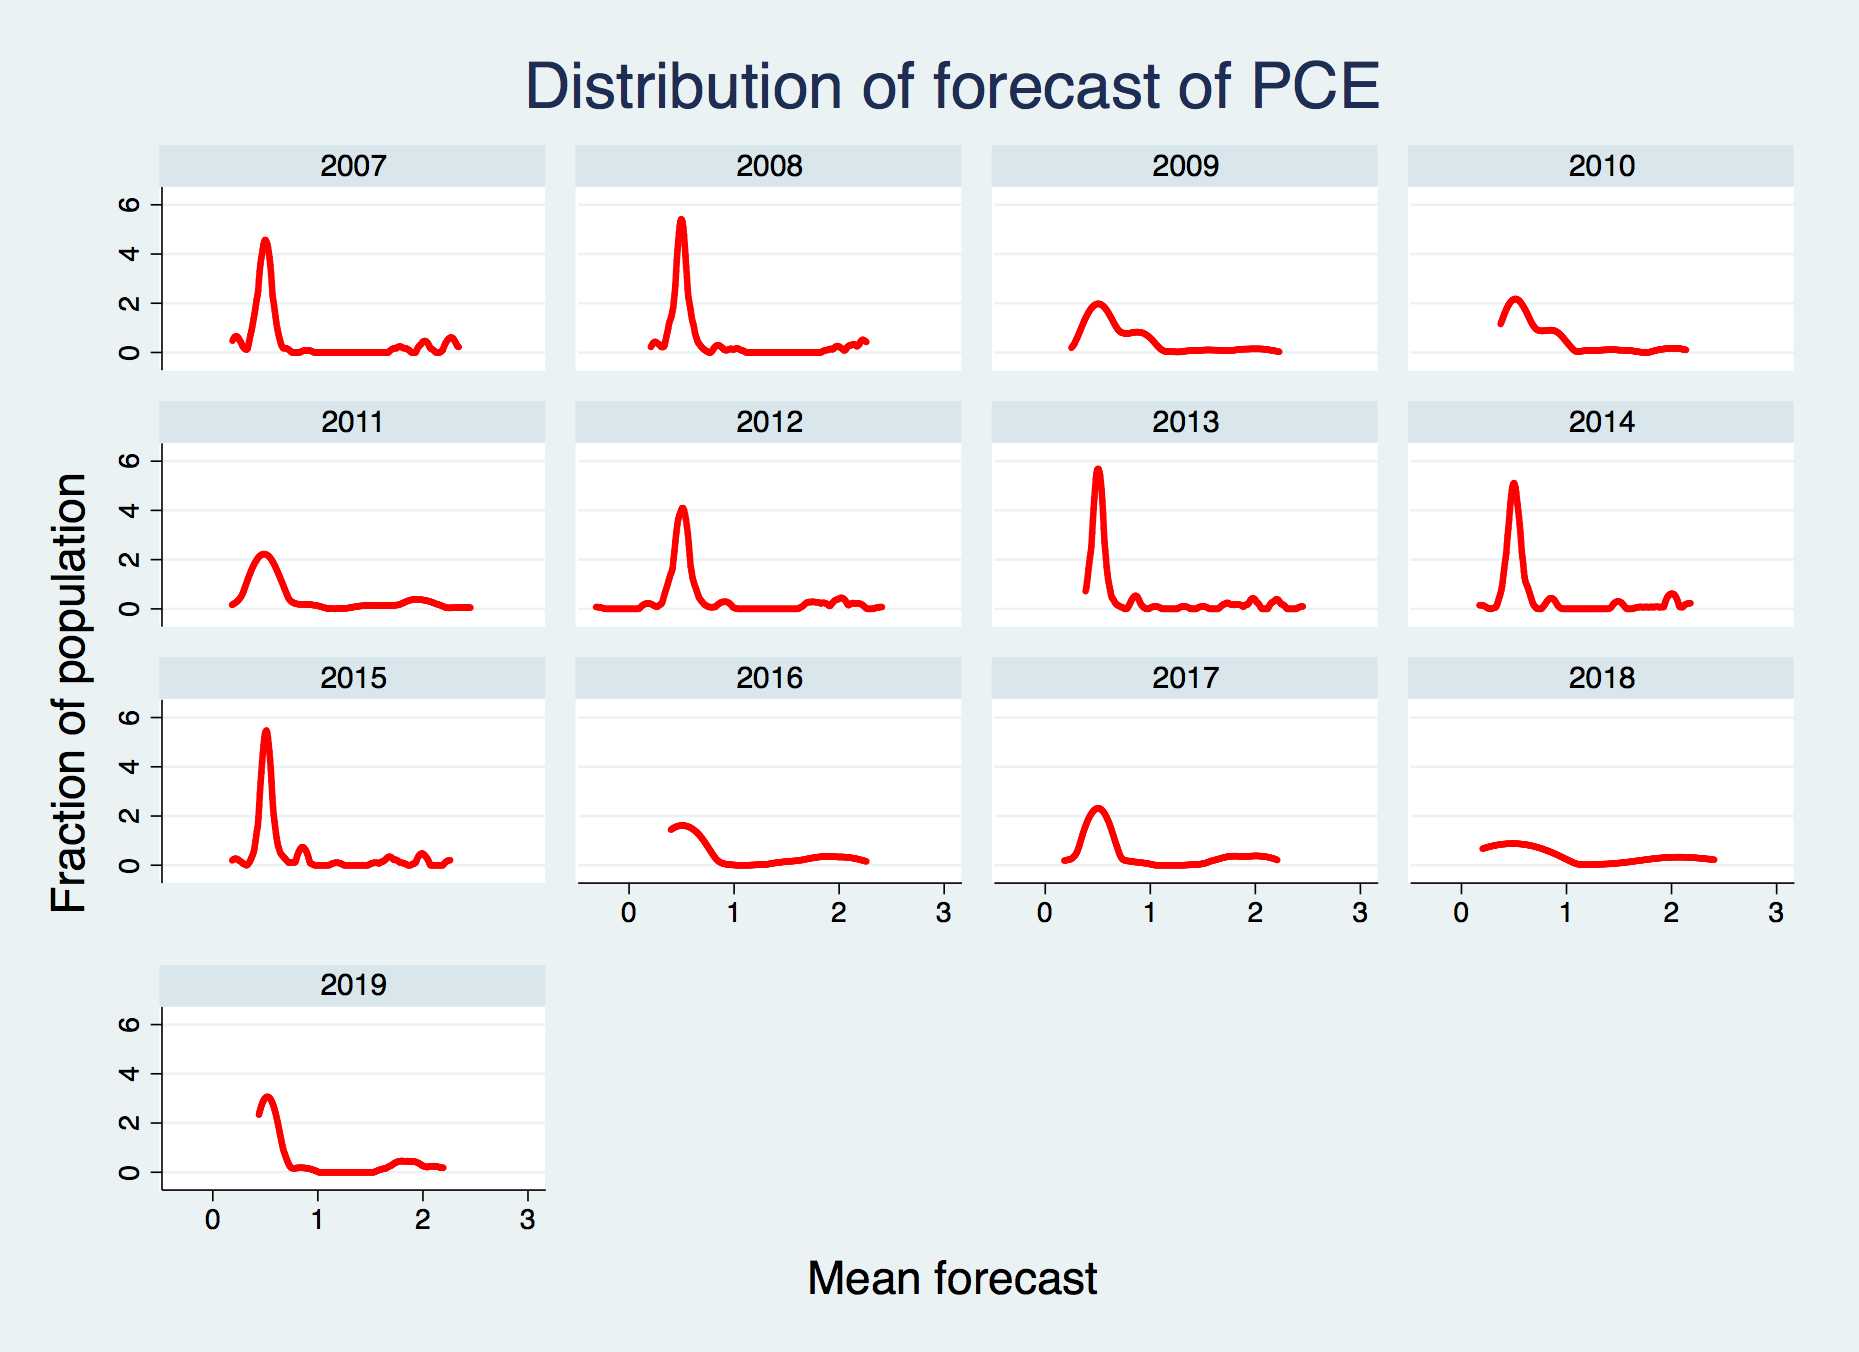
\includegraphics[width=6cm]{figures/PRCPCEMean1_hist.png} 
	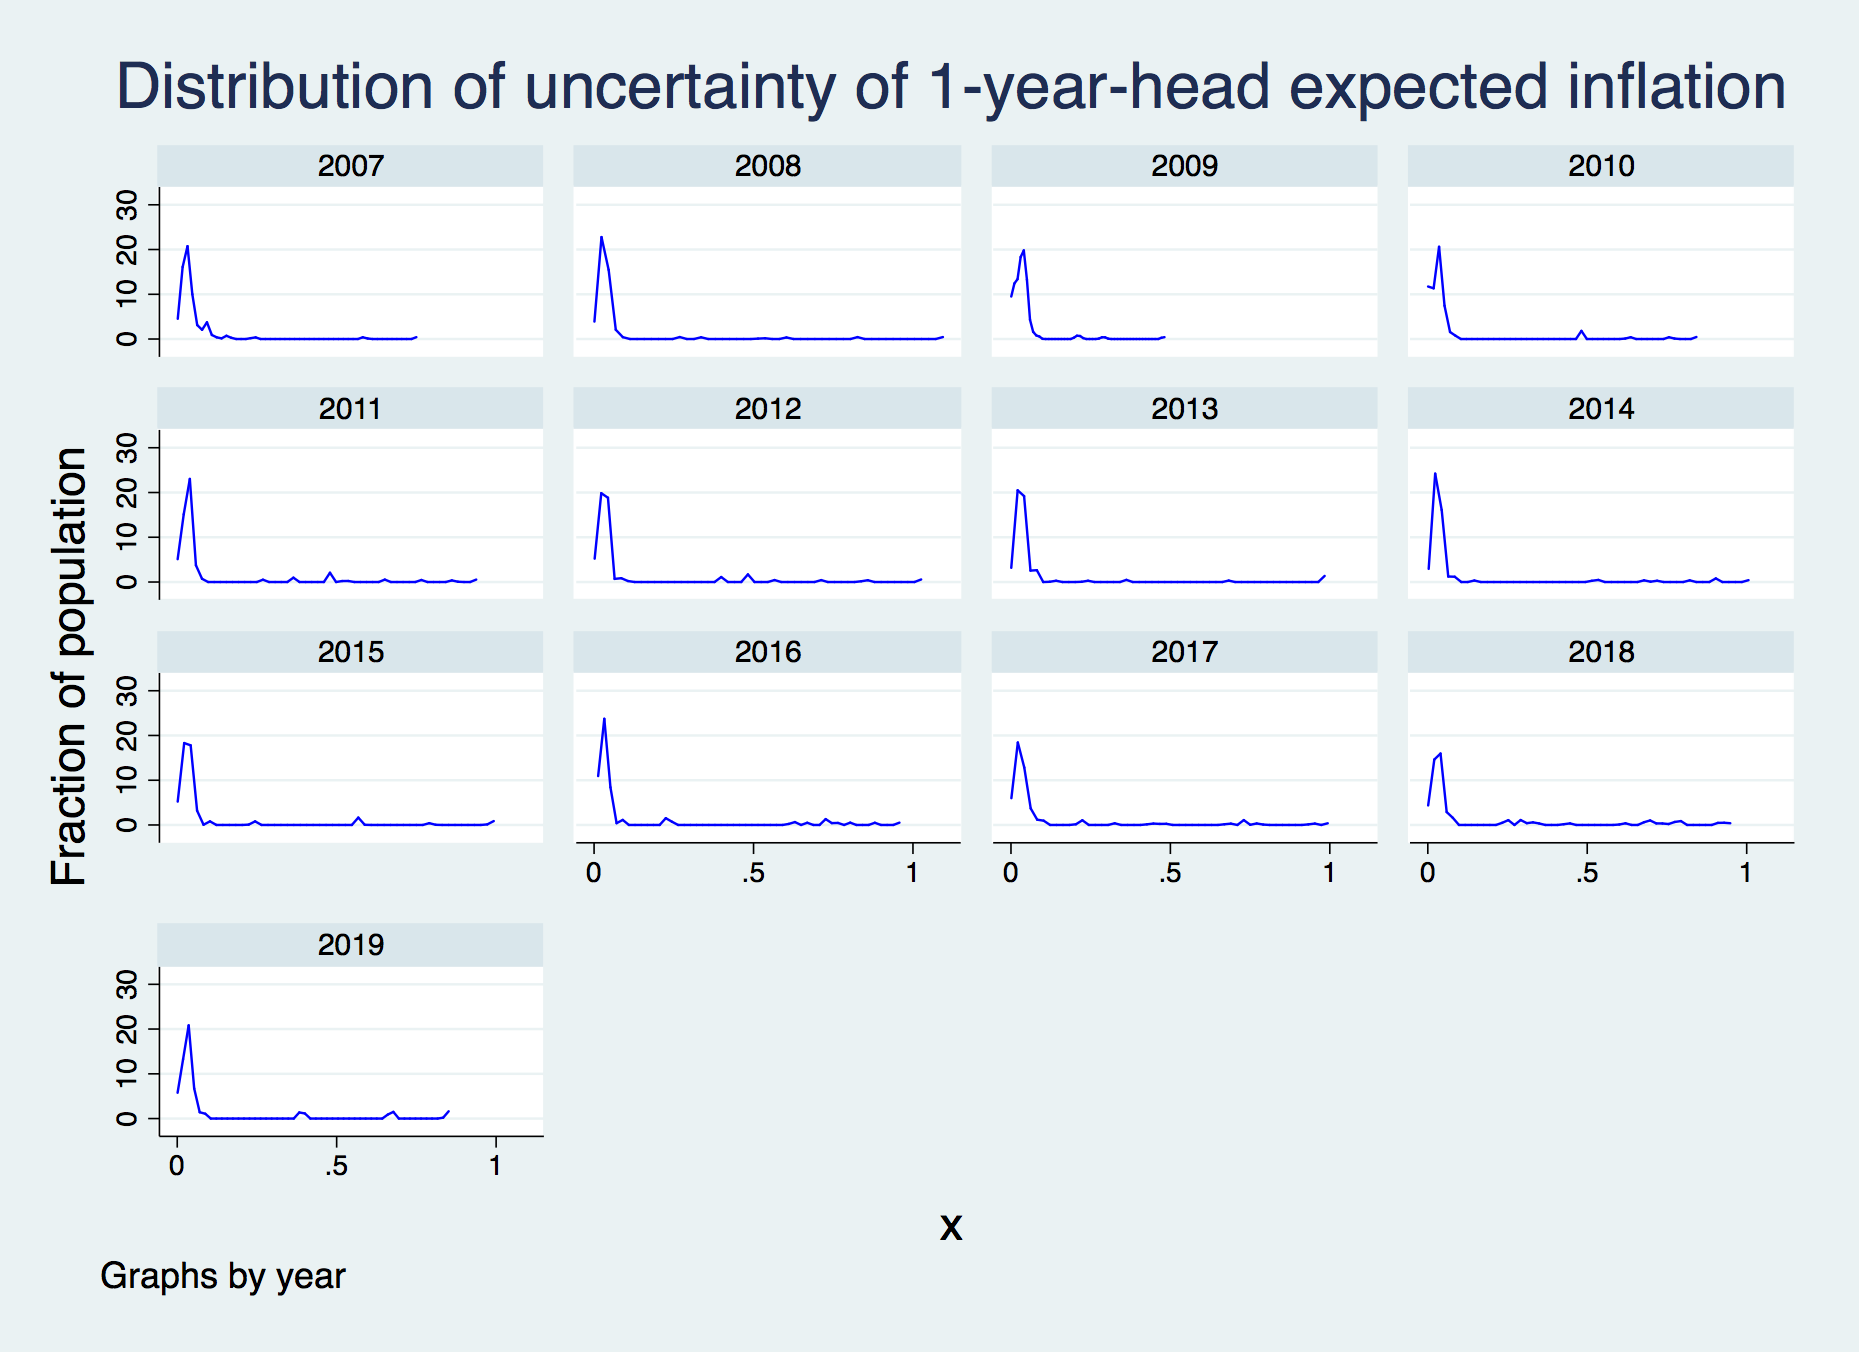
\includegraphics[width=6cm]{figures/PRCPCEVar1_hist.png}  \\
	\smallskip
		\includegraphics[width=6cm]{figures/SCEMean1_hist.png} 
	\includegraphics[width=6cm]{figures/SCEVar1_hist.png}  \\
	\caption{Distribution of Mean Forecast and Uncertainty }
\end{figure}


\begin{figure}[h]\label{RevisionHist}
	\centering
	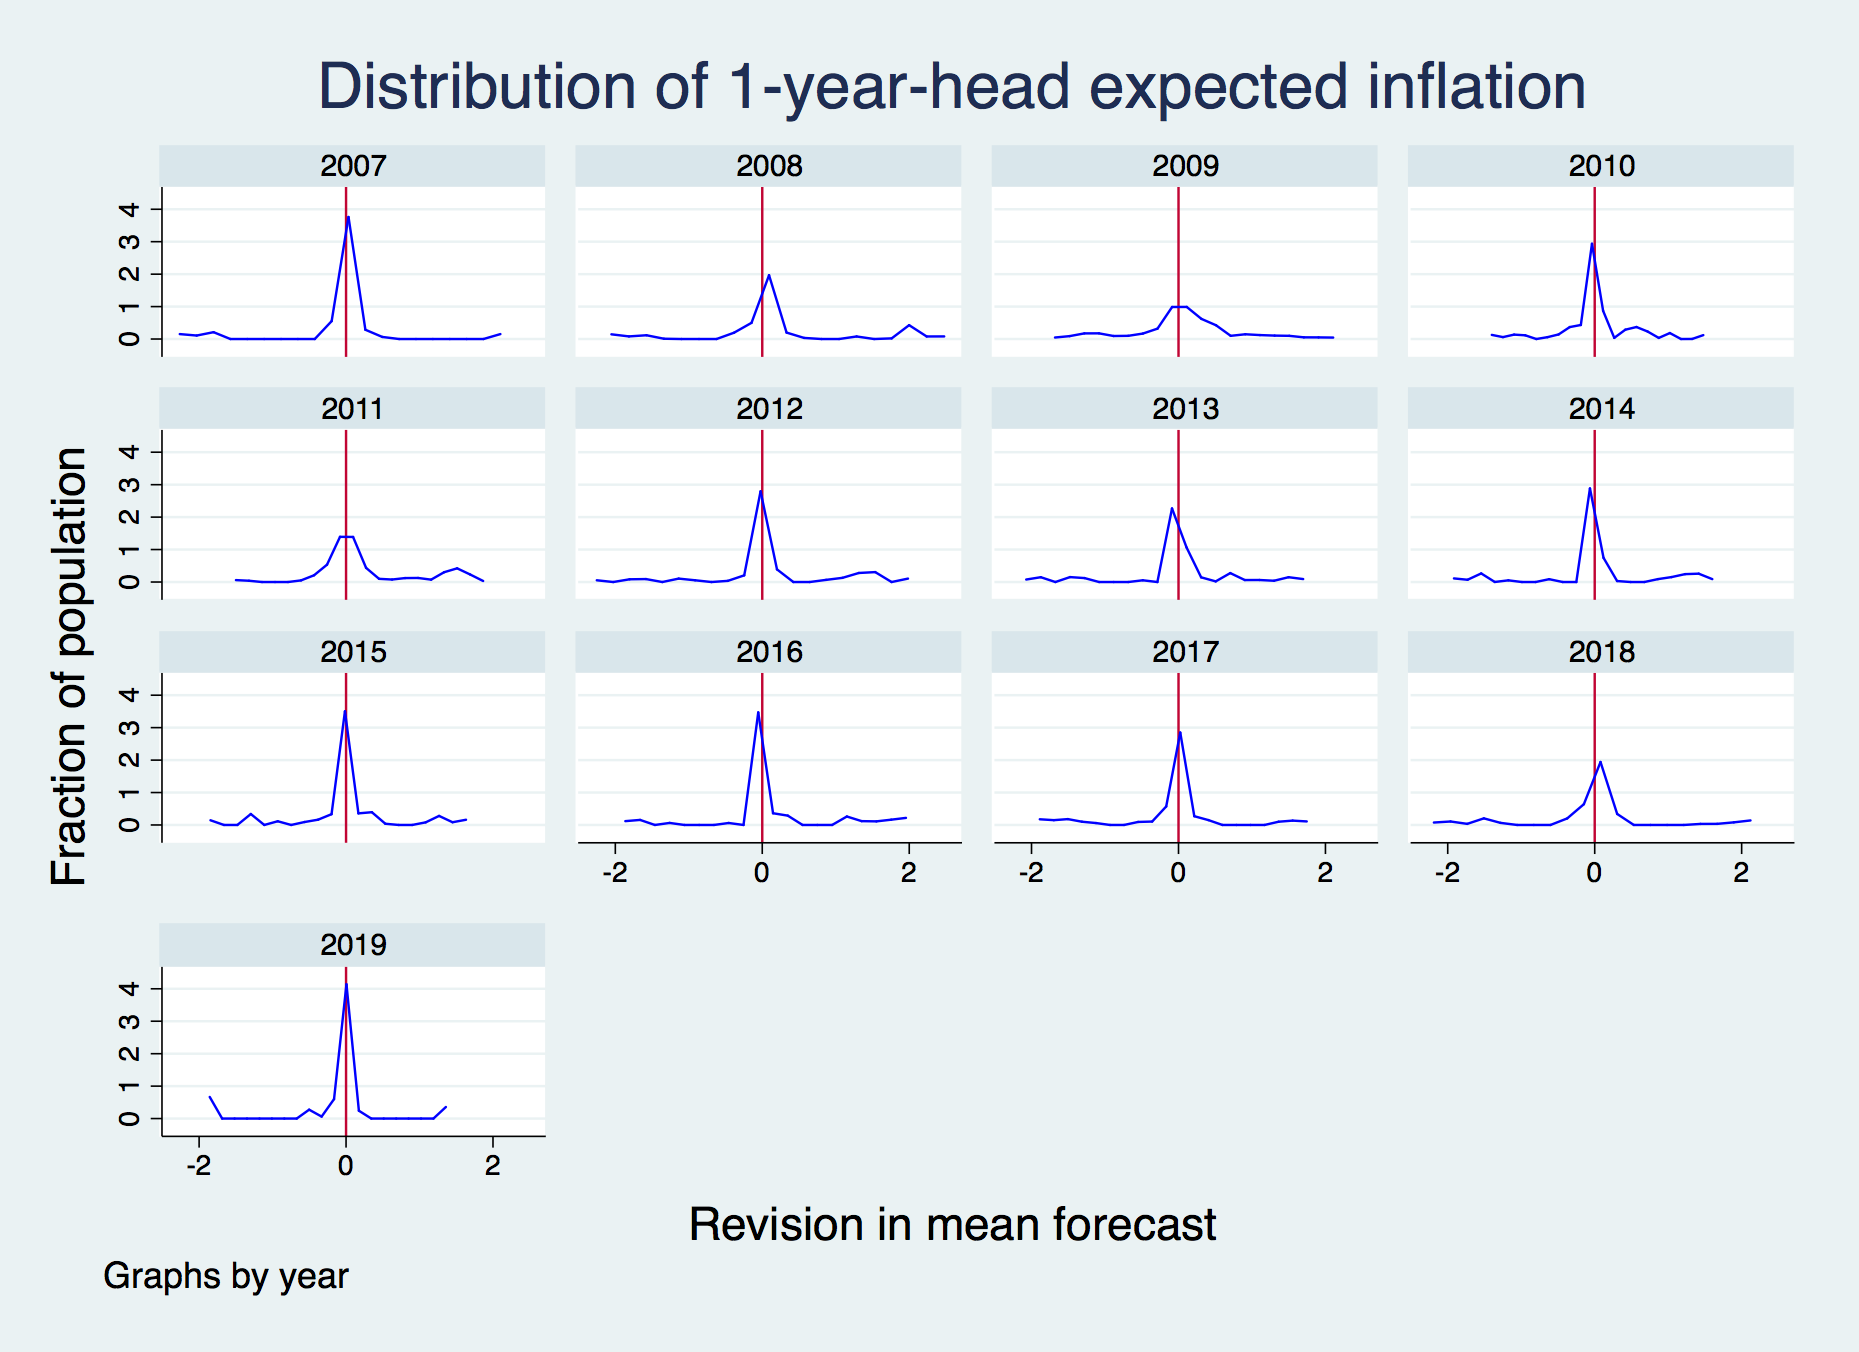
\includegraphics[width=6cm]{figures/PRCCPIMean_rv_hist.png} 
	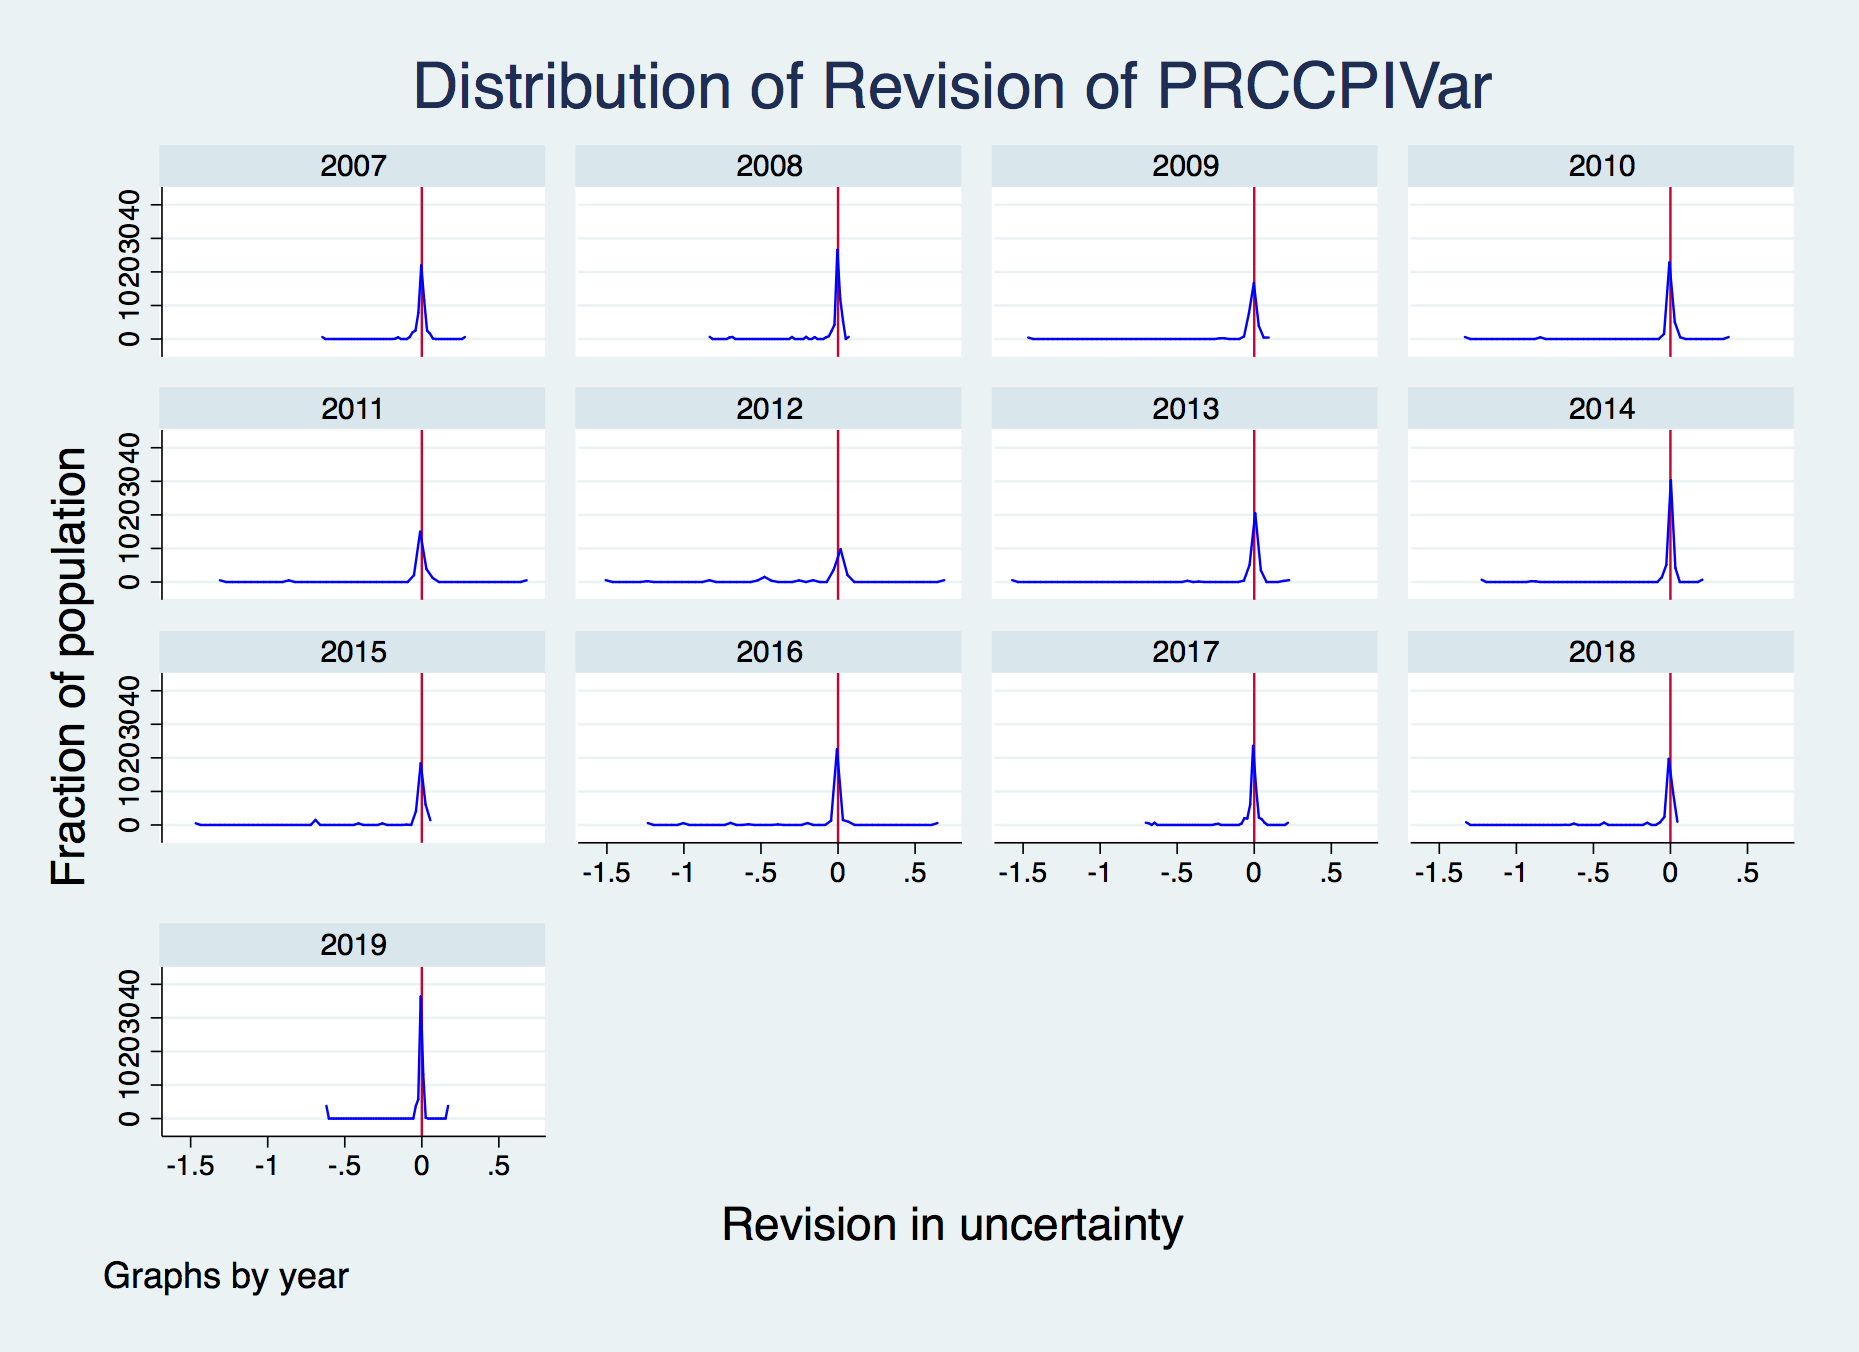
\includegraphics[width=6cm]{figures/PRCCPIVar_rv_hist.png}  \\
	\smallskip
	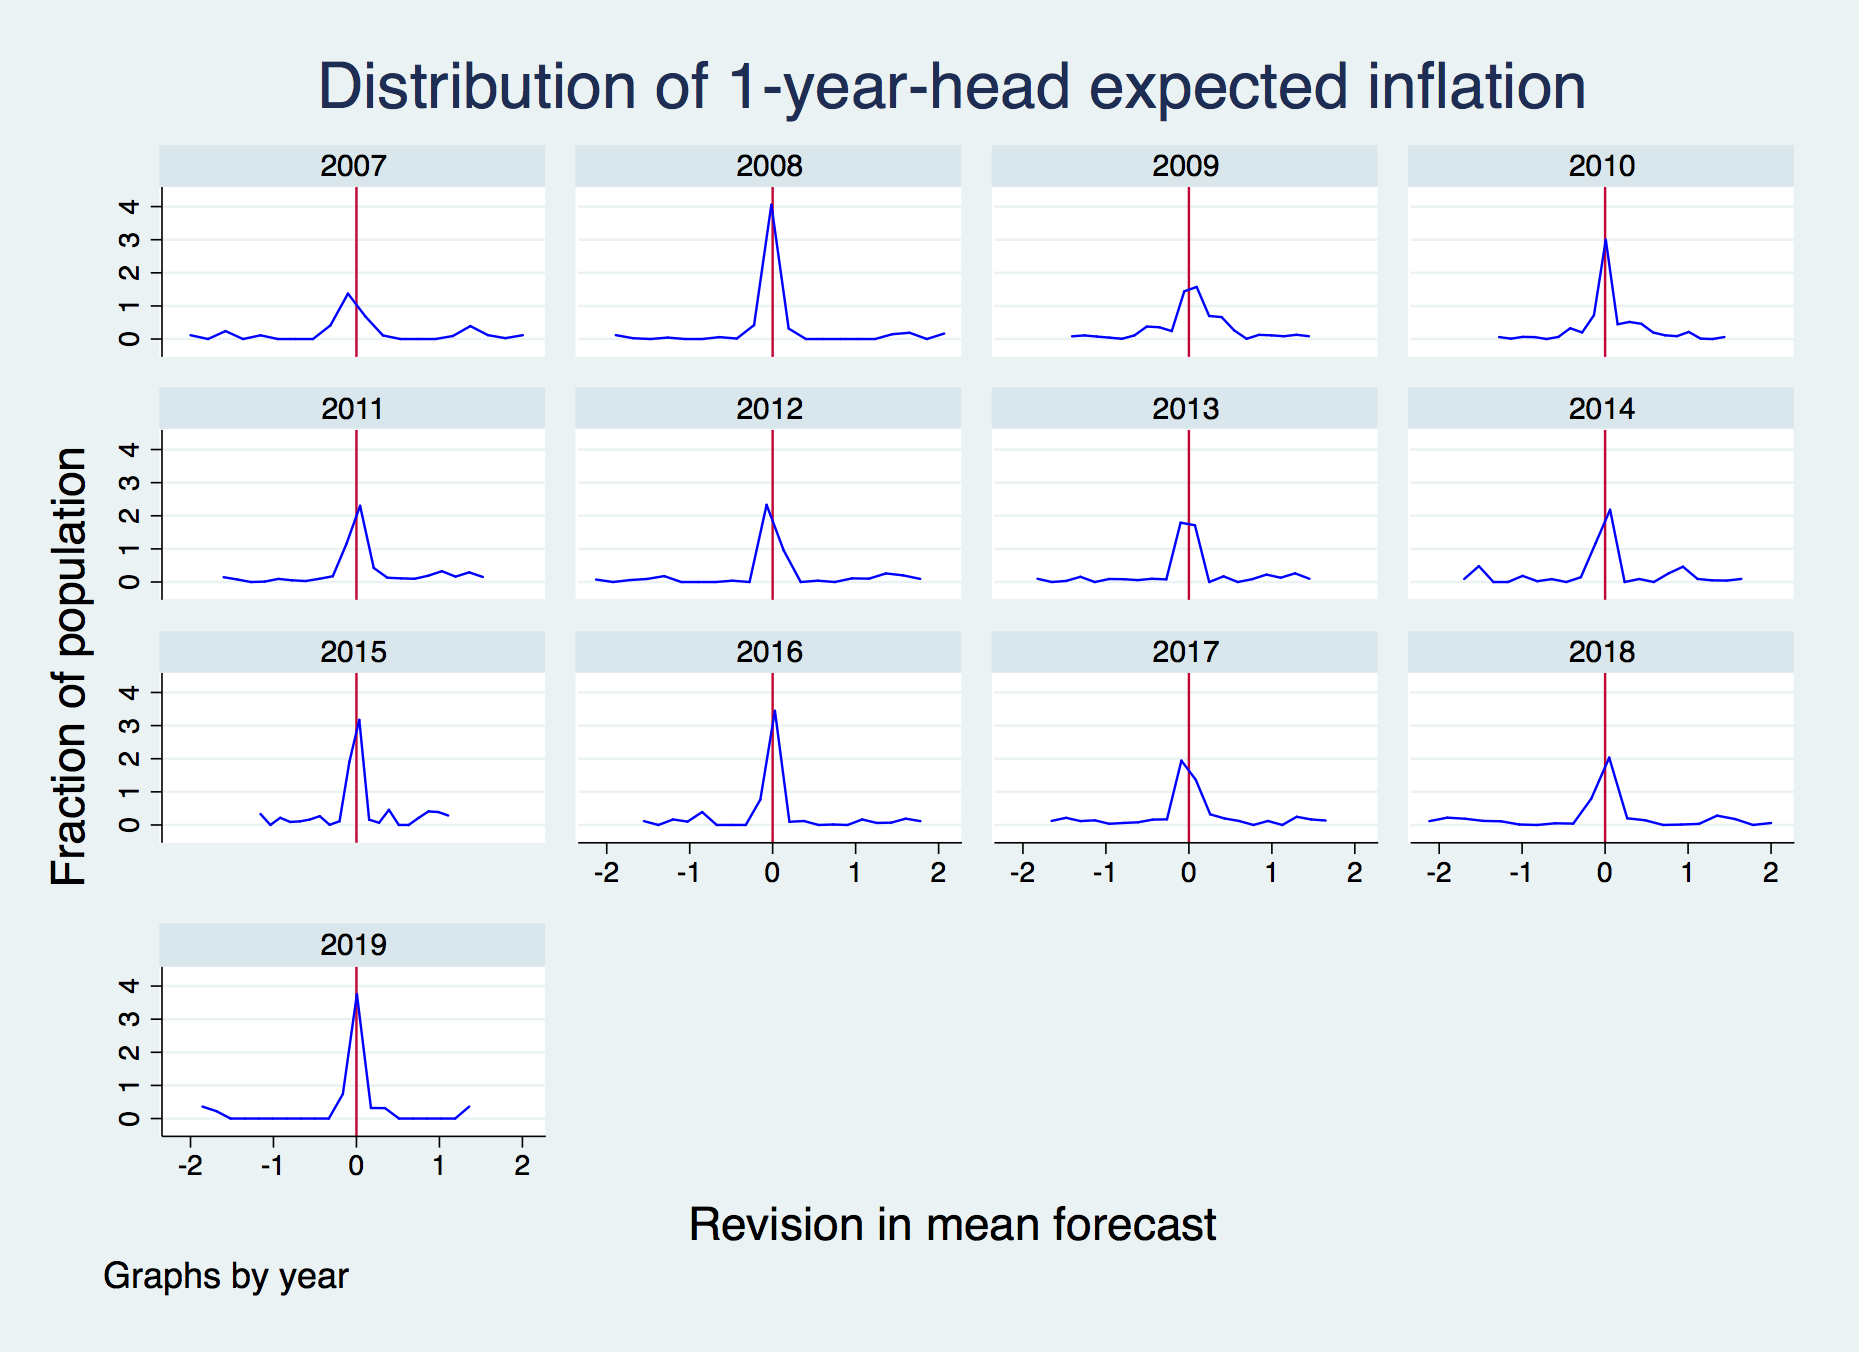
\includegraphics[width=6cm]{figures/PRCPCEMean_rv_hist.png} 
	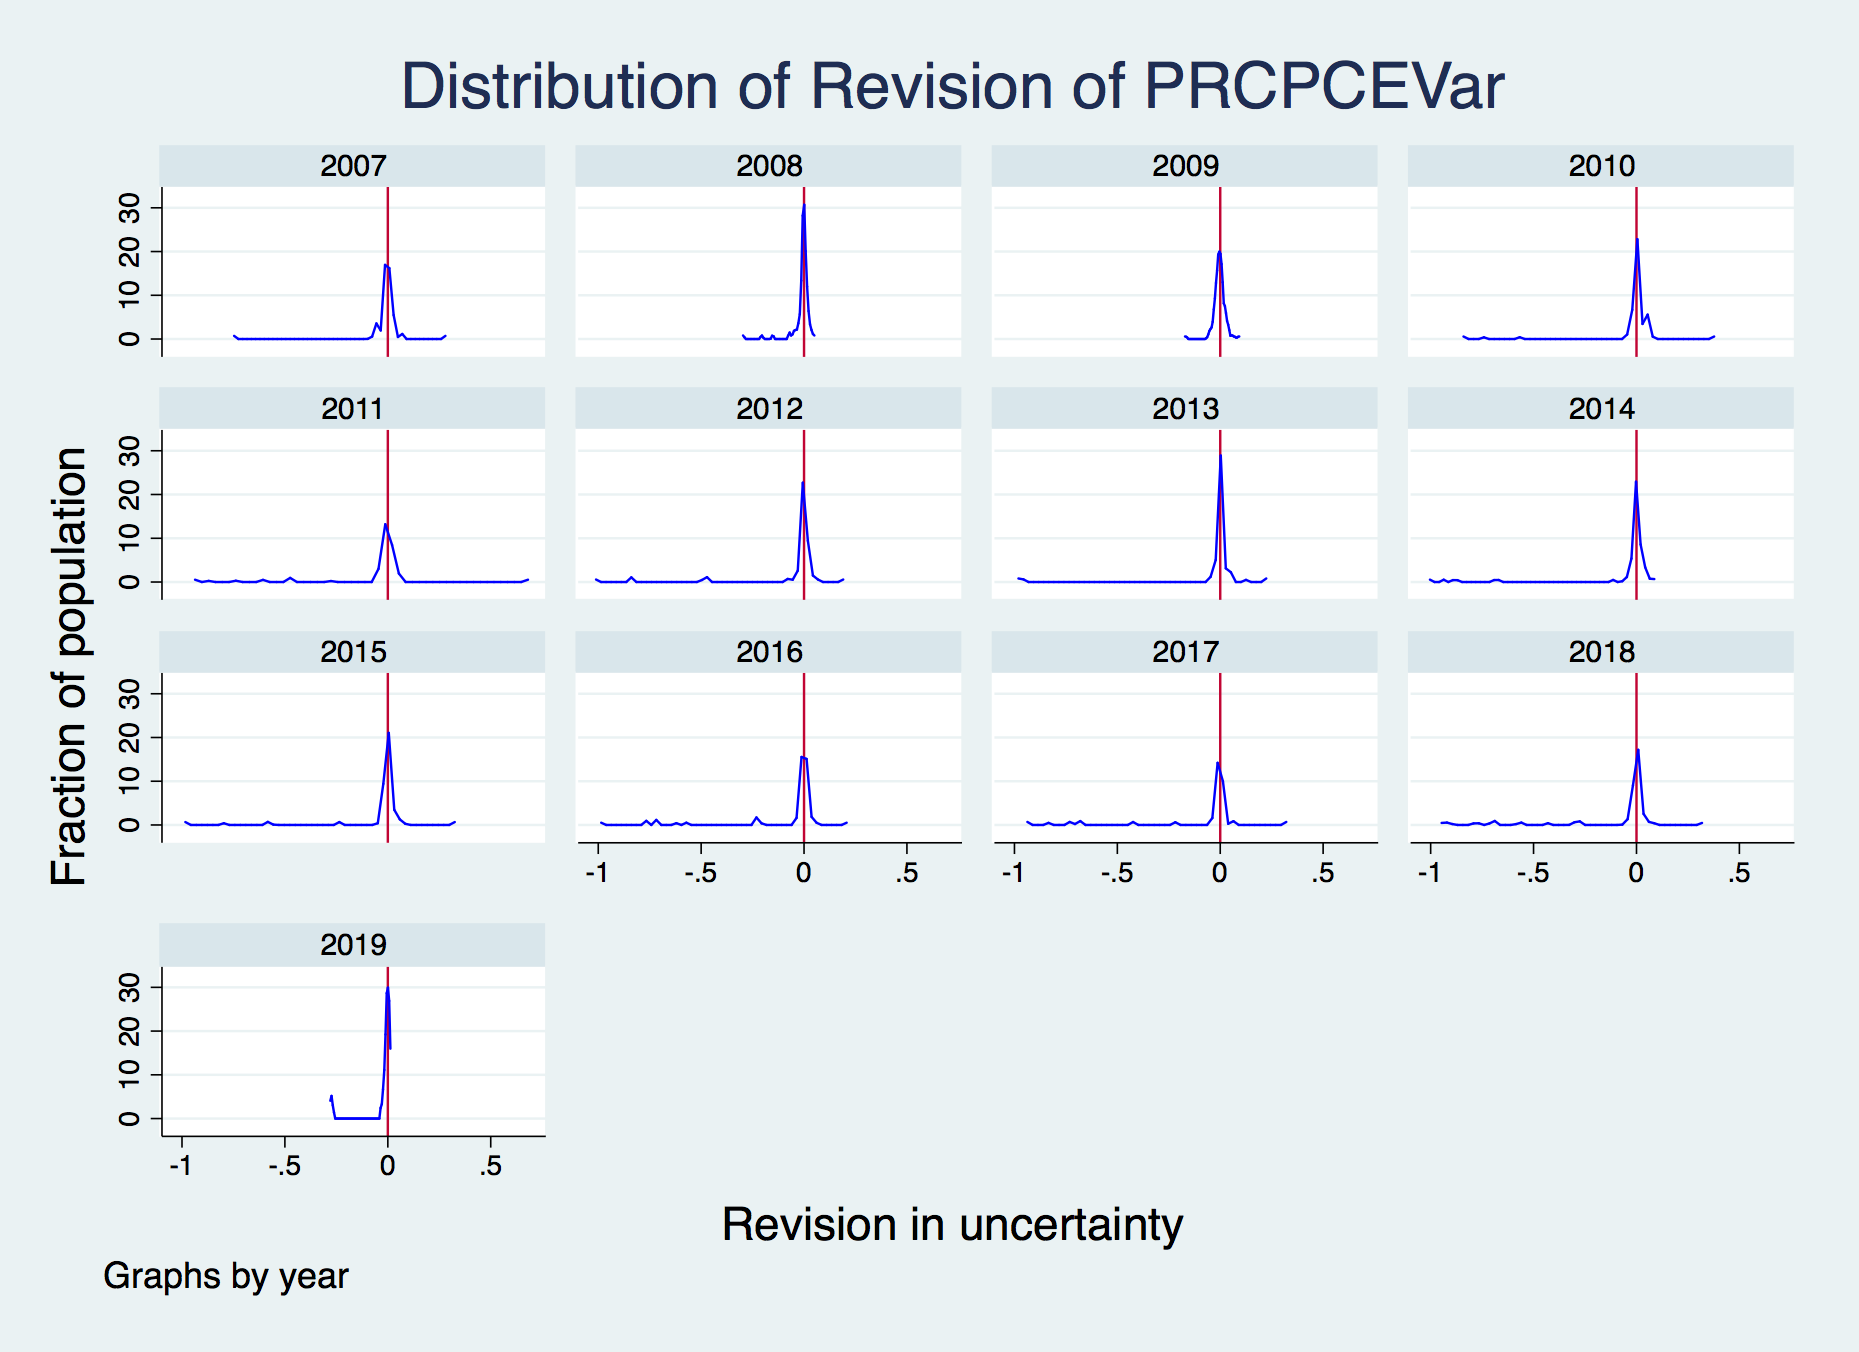
\includegraphics[width=6cm]{figures/PRCPCEVar_rv_hist.png}  \\
	\smallskip
		\includegraphics[width=6cm]{figures/SCEMean_rv_hist.png} 
	\includegraphics[width=6cm]{figures/SCEVar_rv_hist.png}  \\
	\caption{Distribution of Revision in Forecasts}
\end{figure}

\subsection{Test of Null Hypothesis of Rational Expectation}

In Table \ref{NullTestTable}, I reproduce a number of commonly used tests of null hypothesis of FIRE replying on differnet specific implications discussed in the previous section. I first reproduce the results from two papers, \cite{mankiw2003disagreement} and \cite{fuhrer2018intrinsic} and then proceed to show the results with the additional restrictions from ucnertainty. 

The first set of tests utilize the dynamics of forecast errors. First, the forecast error should be on average unbiased. The forecast error should converge to zero. Second, forecast errors of non-overlapping forecasting horizon are not serially correlated.  Third, forecast errors should not be predicted by any information available at the time of forecast, including the forecast itself and other variable that is in the agent's information content. 

The second batch of tests focus on  forecasting efficiency utilizing revision across different vintages of forecasts in the spirit of \cite{nordhaus1987forecasting}. In particular, I follow the model specifications in \cite{fuhrer2018intrinsic}. According to FIRE, rational forecast revision only responds to newly realized shocks thus it cannot be predicted by past information. For the same reason, regression coefficient of forecast for $y_{t+h}$  at time $t+1$ on that at $t-1$ is exactly equal to $1$, implying one-to-one responses.  A weaker test in the similar test is that the change in mean forecast from one period to the next one fixing forecasting horizon is serially correlated to an greater extent than that comes from the additional period in far future. 

\begin{table}[]\label{NullTestTable}
	\caption{Test of Rationality and Efficicency}
	\centering 
	\begin{tabular}{lll}
		
		\hline 
		& SCE & SPF        \\
		\hline 
		                                  &                             &             \\
	\end{tabular}
\end{table}


\subsection{Professional Forecasters as a Benchmark}

\subsubsection{Replicating \cite{coibion2012can}}

In Figure \ref{ReplicateCoibionBefore2007}, I replicate the results from  \cite{coibion2012can}. The period is between 1987-2007.  In the right column, I do the same exercise with monetary policy shocks. 

In Figure \ref{ReplicateCoibionpost2007}, I do the same exercise but include additional uncertainty. This is also the period when SPF provides density forecasts that allow me to estimate uncertainty. 

\begin{figure}[h]\label{ReplicateCoibionBefore2007}
	\centering
	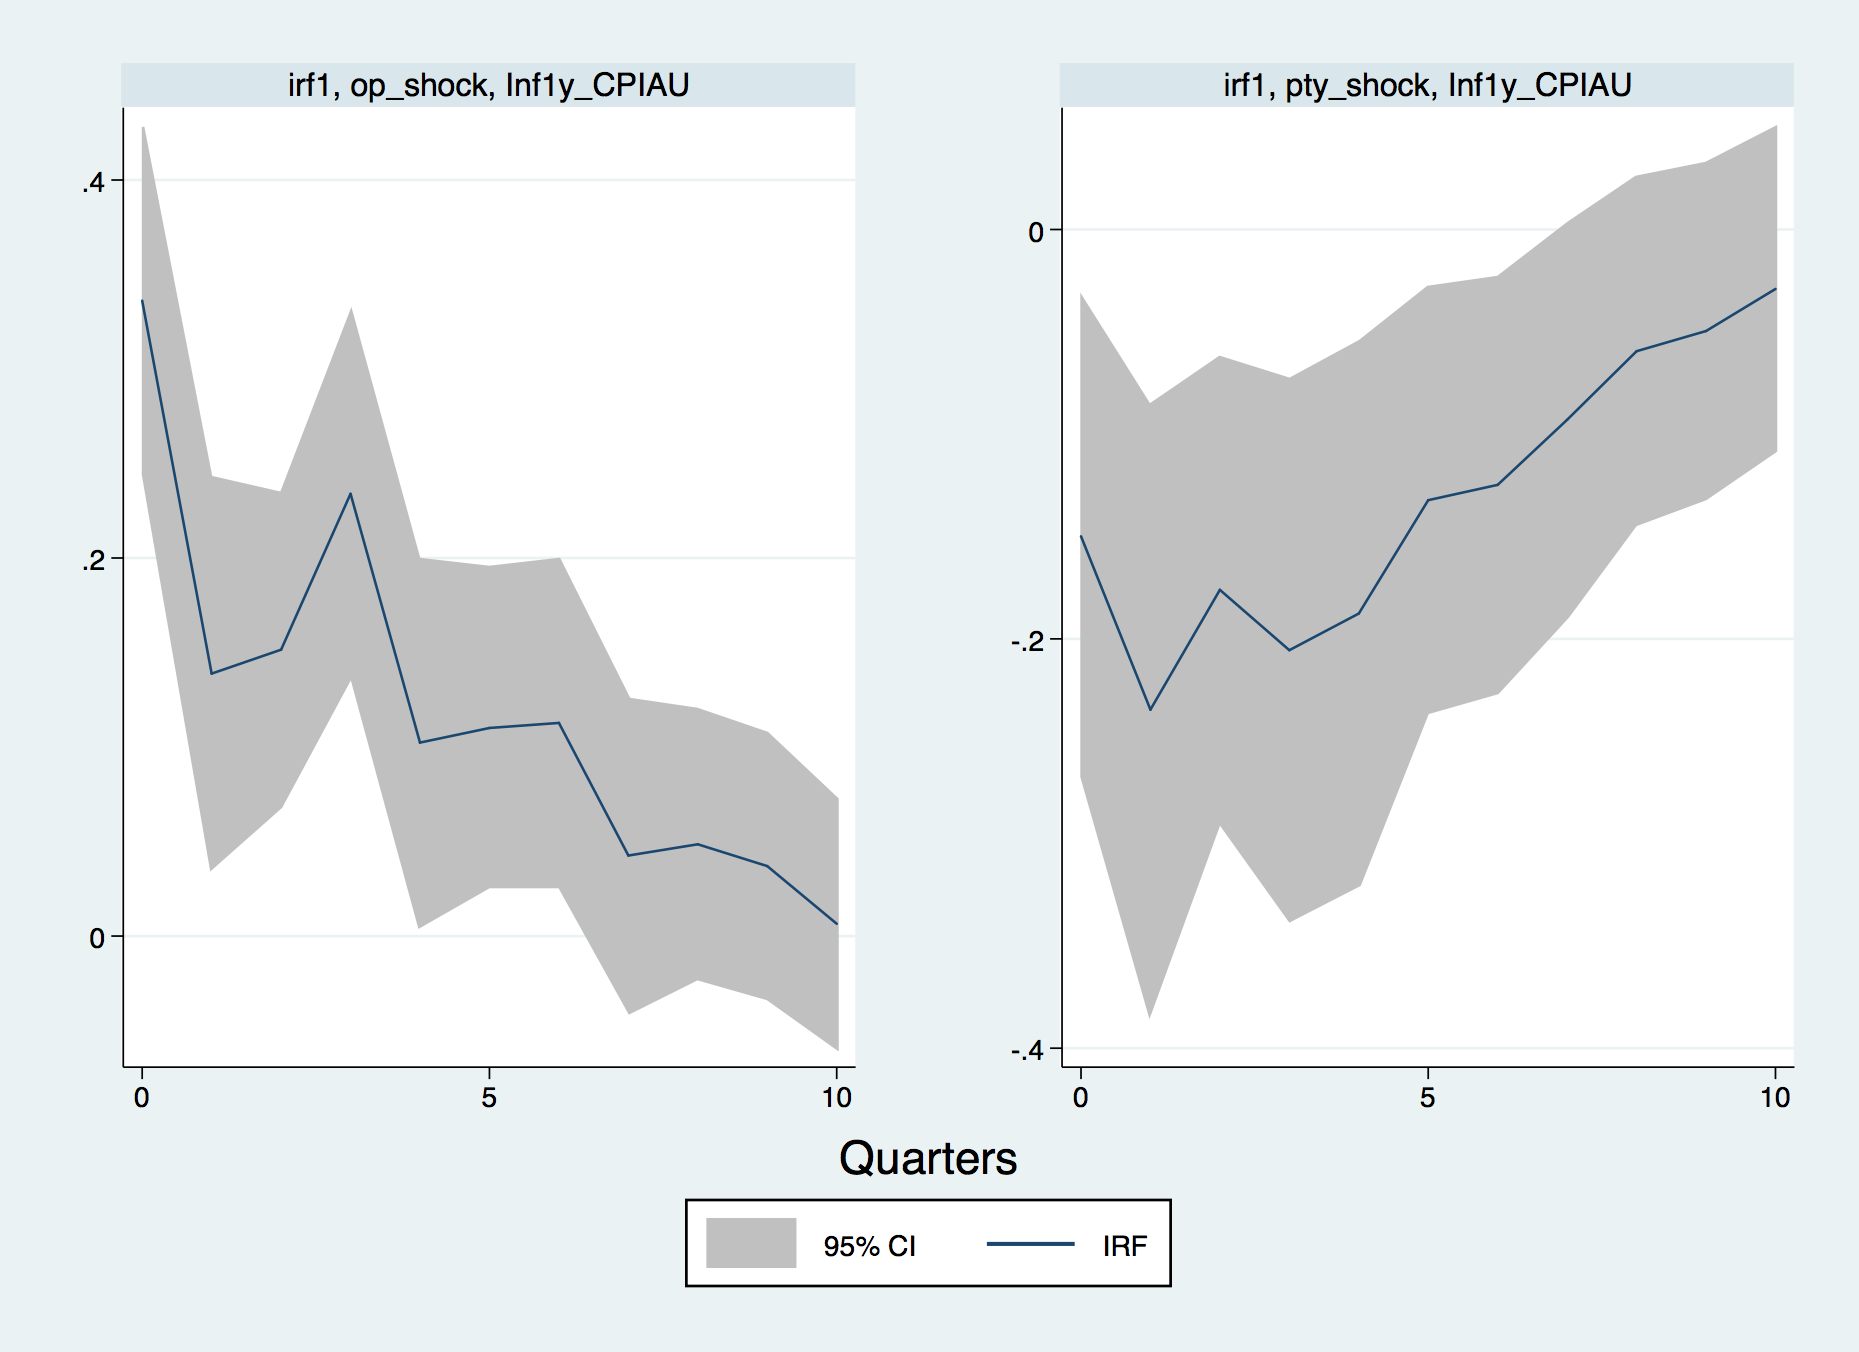
\includegraphics[width=6cm,height=2cm]{figures/CPIAU_ashocks_nmp.png}  
	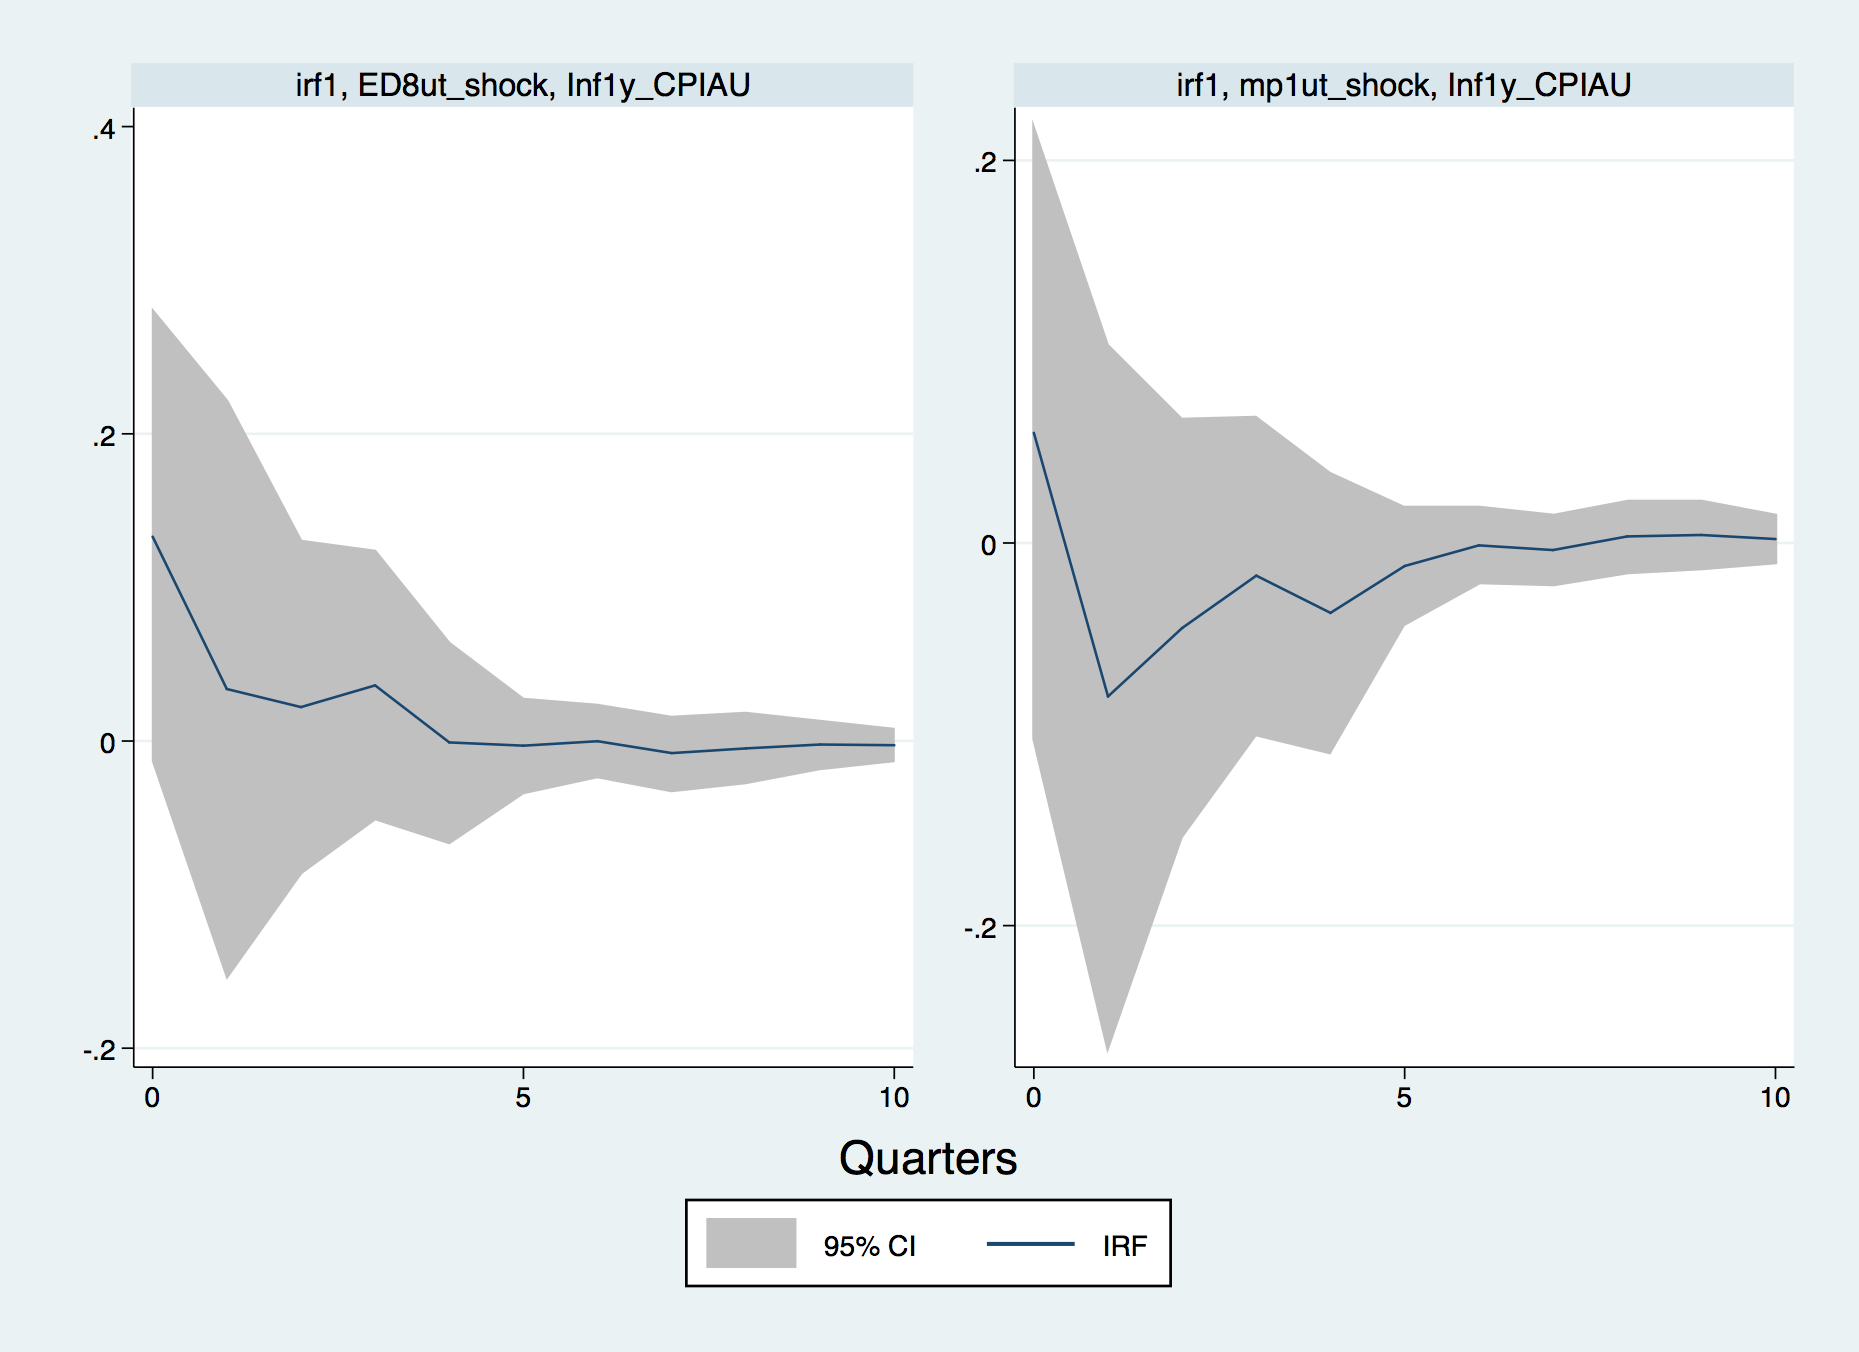
\includegraphics[width=6cm,height=2cm]{figures/CPIAU_ashocks.png} \\
	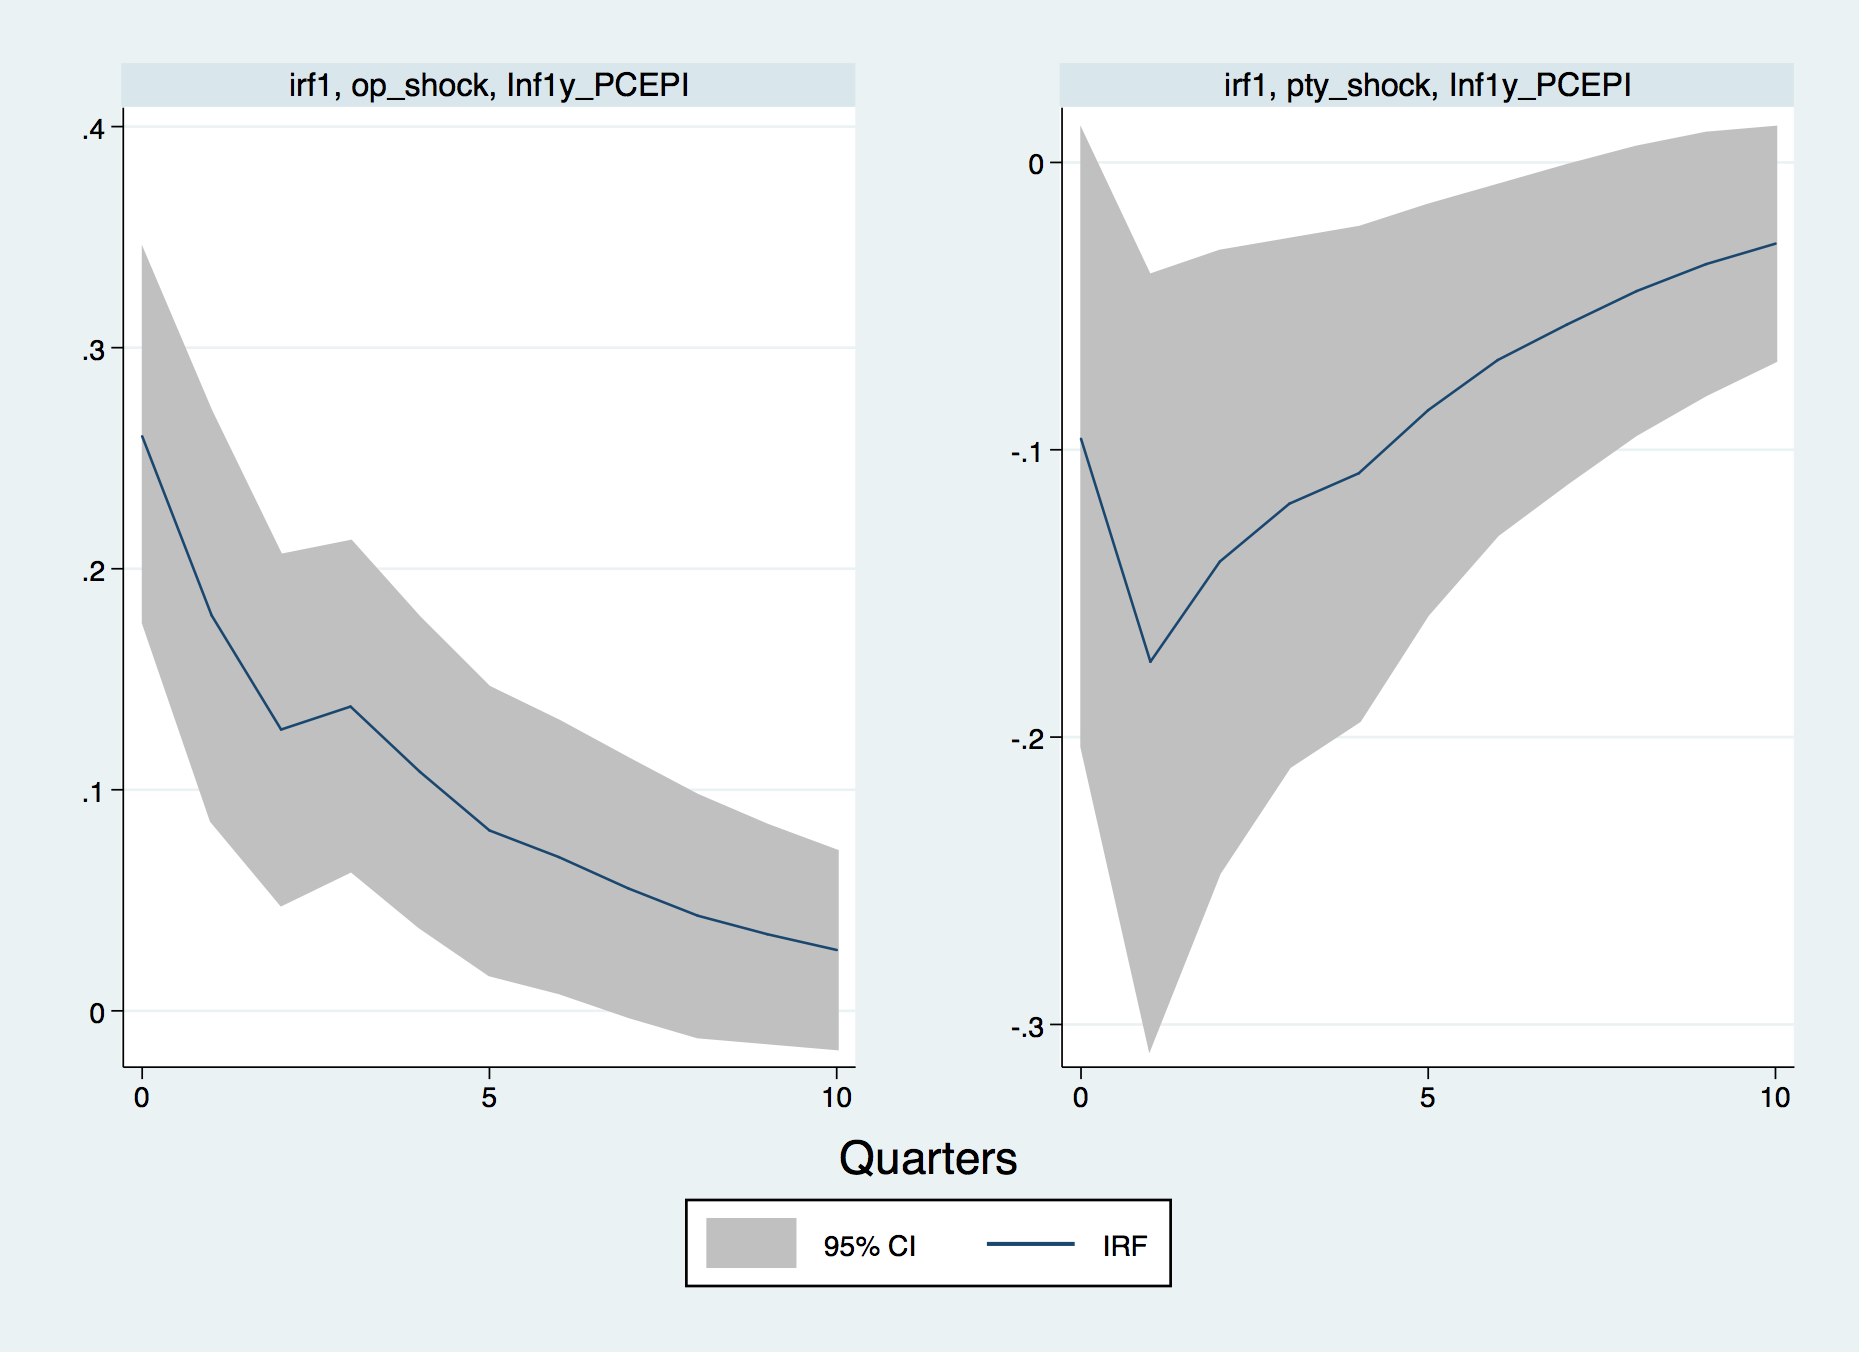
\includegraphics[width=6cm,height=2cm]{figures/PCEPI_ashocks_nmp.png} 
	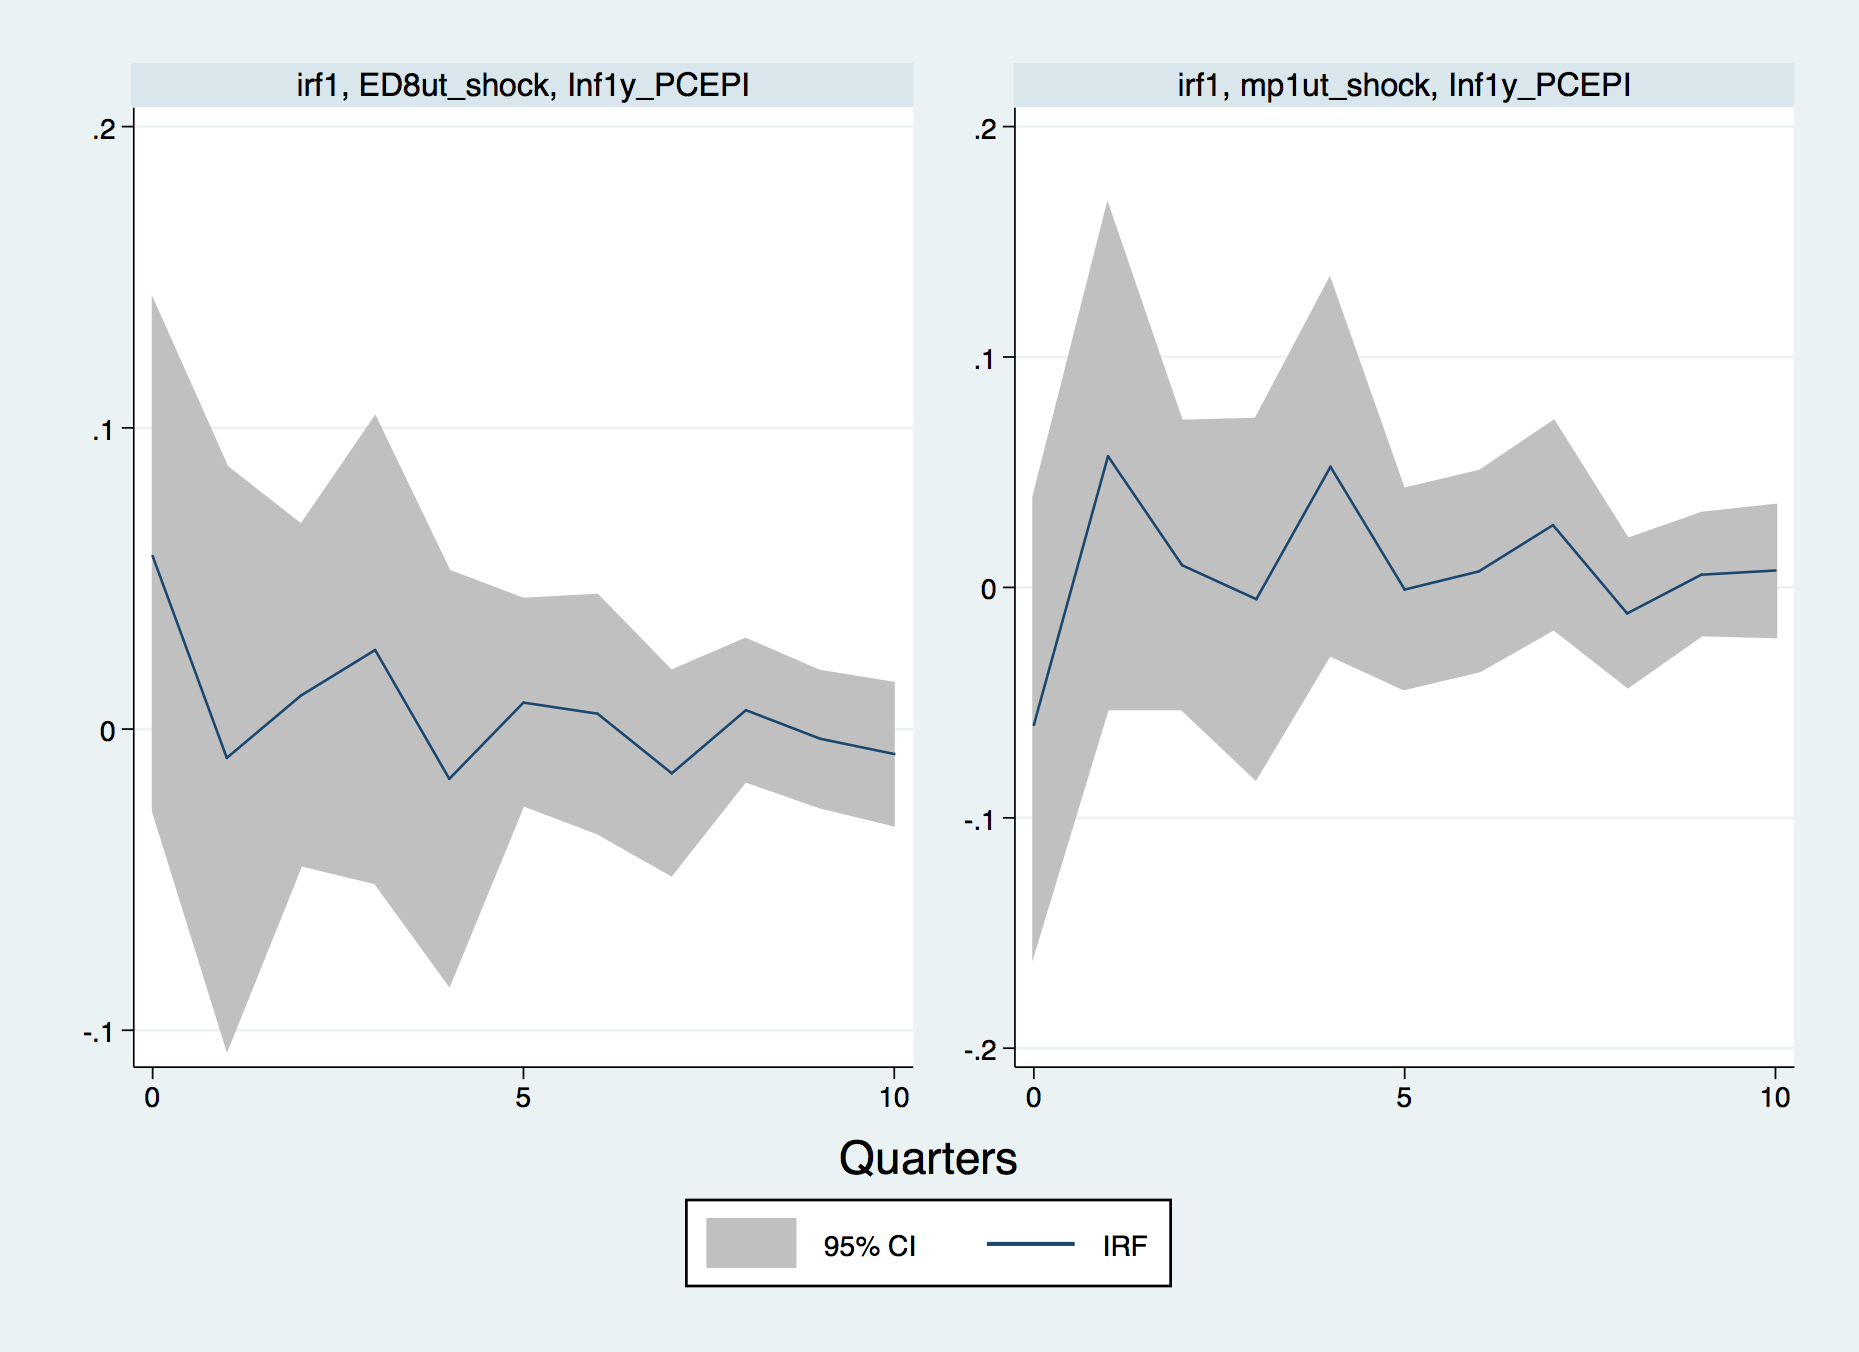
\includegraphics[width=6cm,height=2cm]{figures/PCEPI_ashocks.png}  \\
	\smallskip
	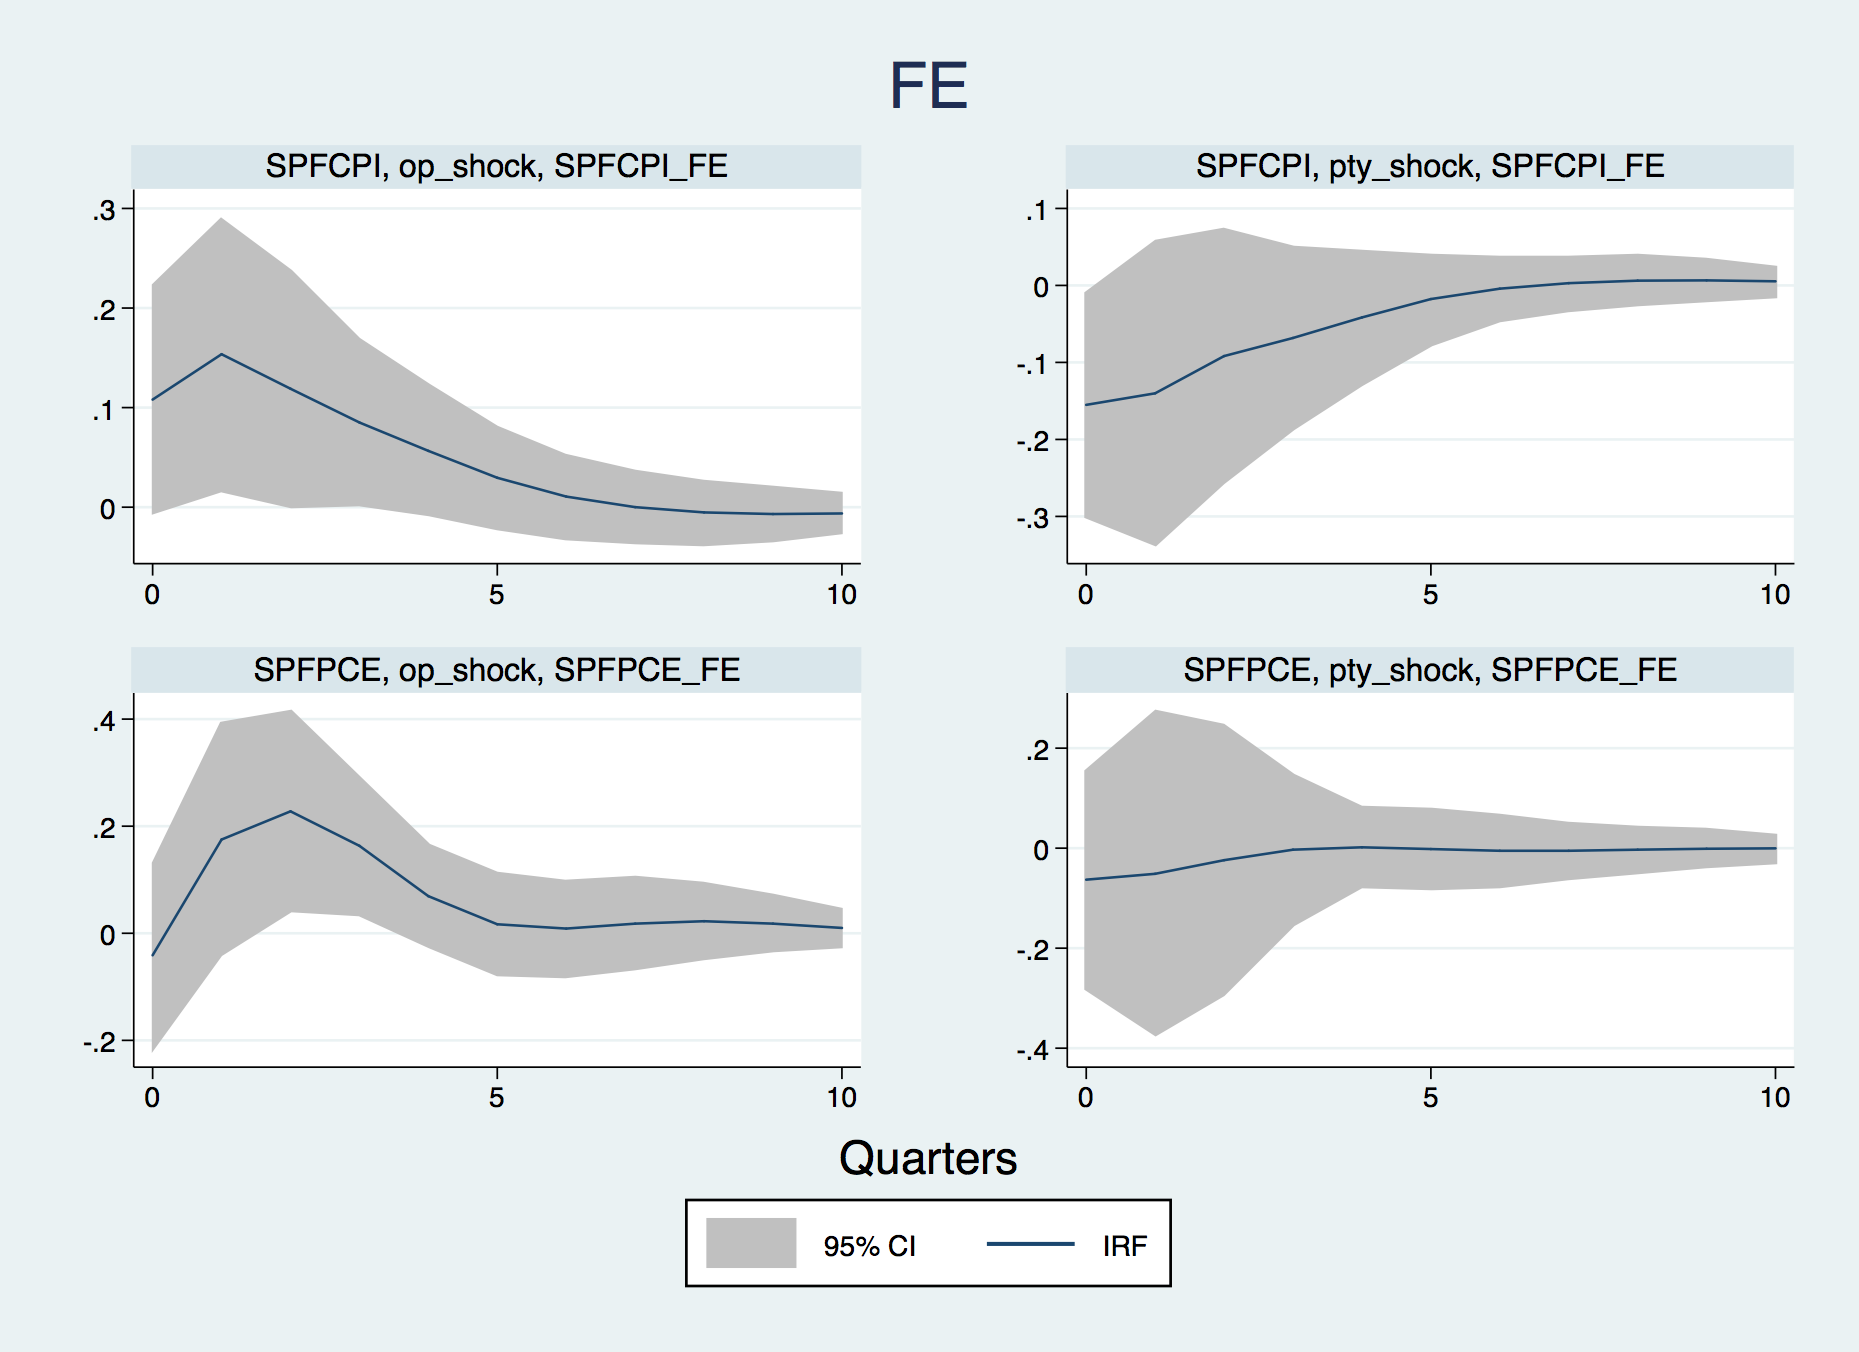
\includegraphics[width=6cm]{figures/SPFFE_ashocks_nmp.png} 
		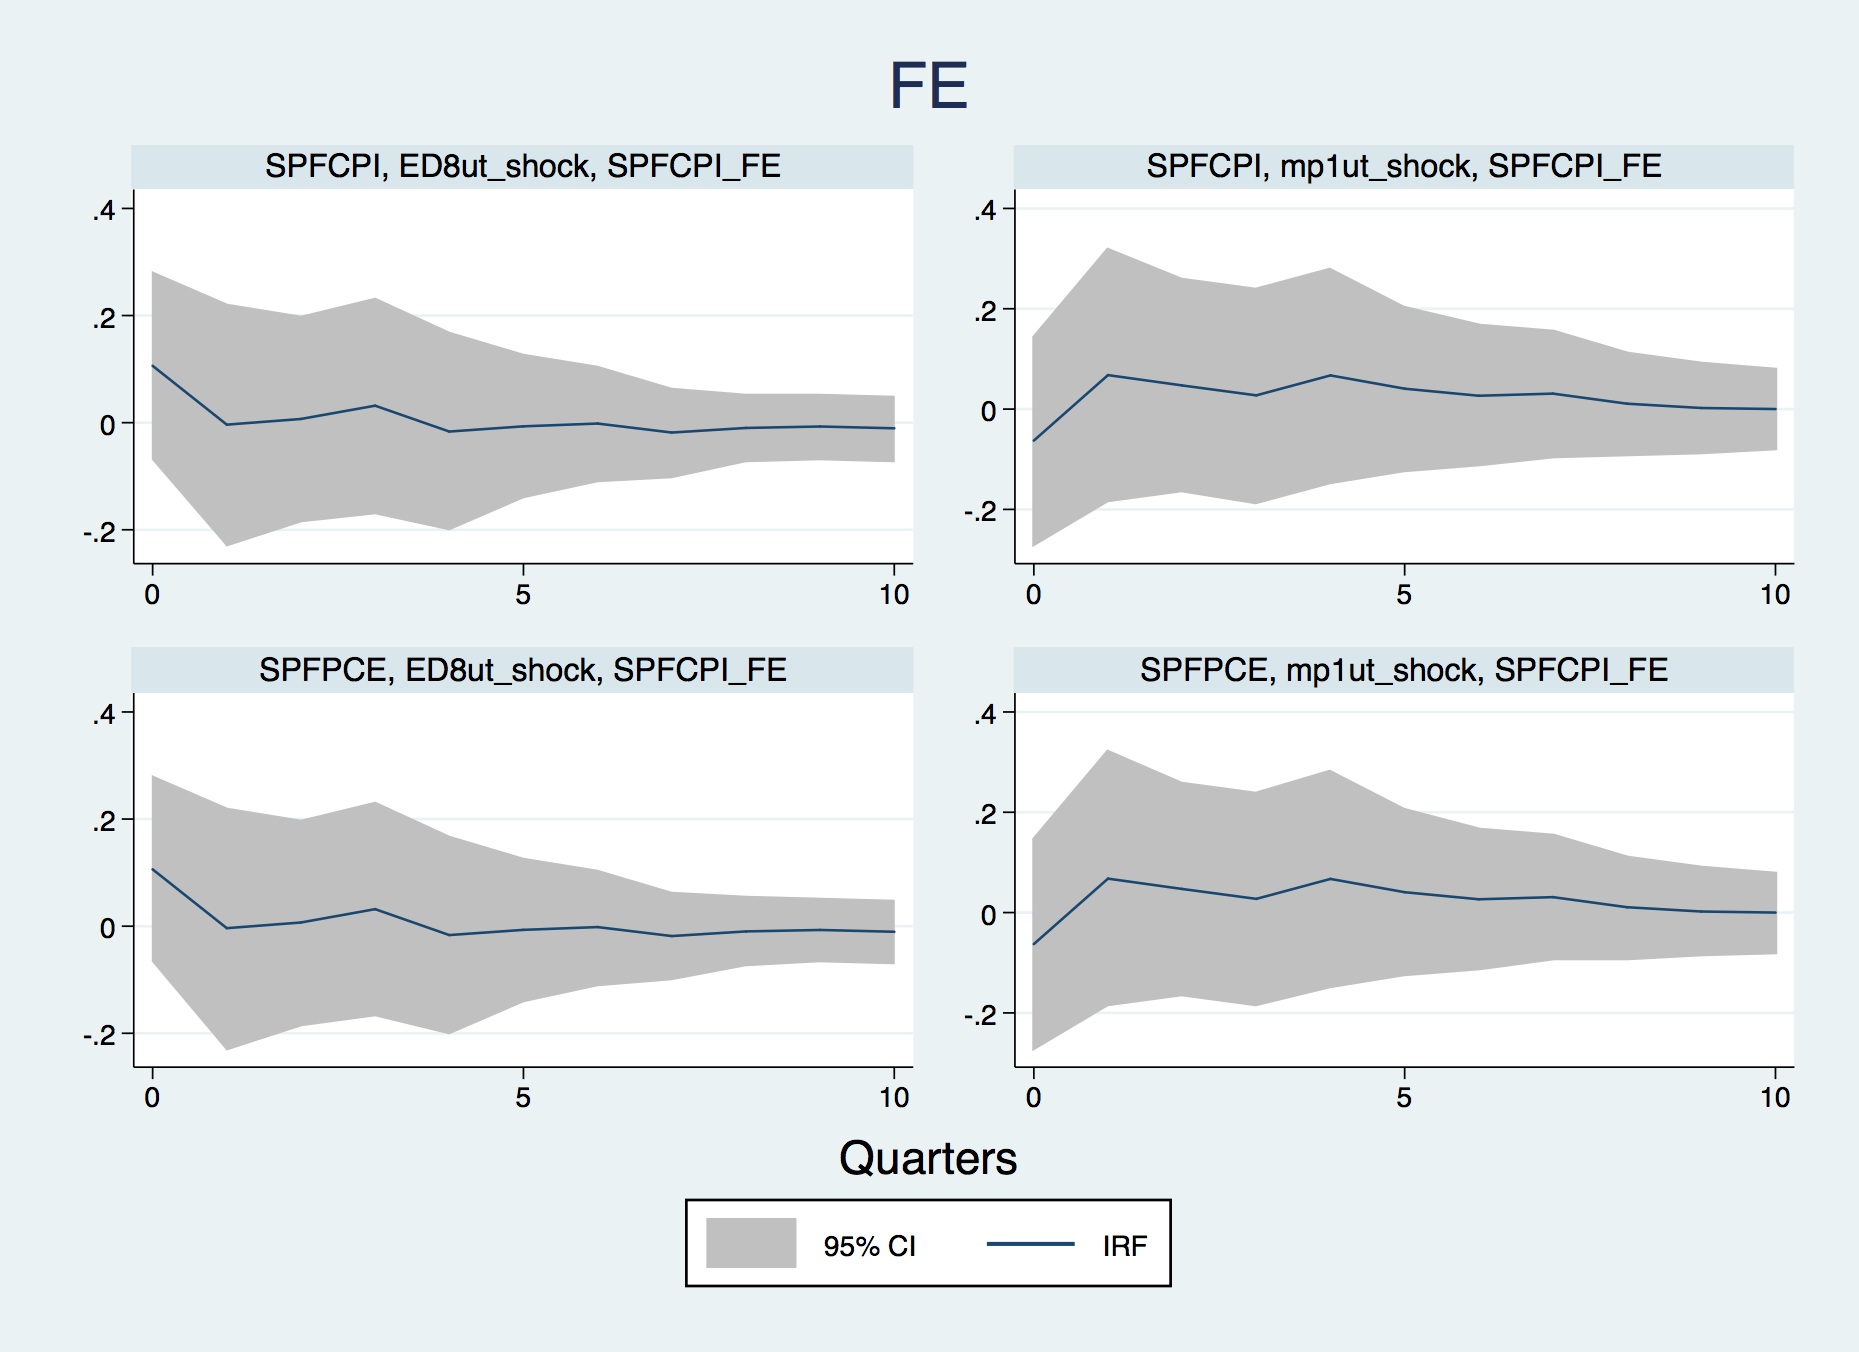
\includegraphics[width=6cm]{figures/SPFFE_ashocks.png} \\
	\smallskip
	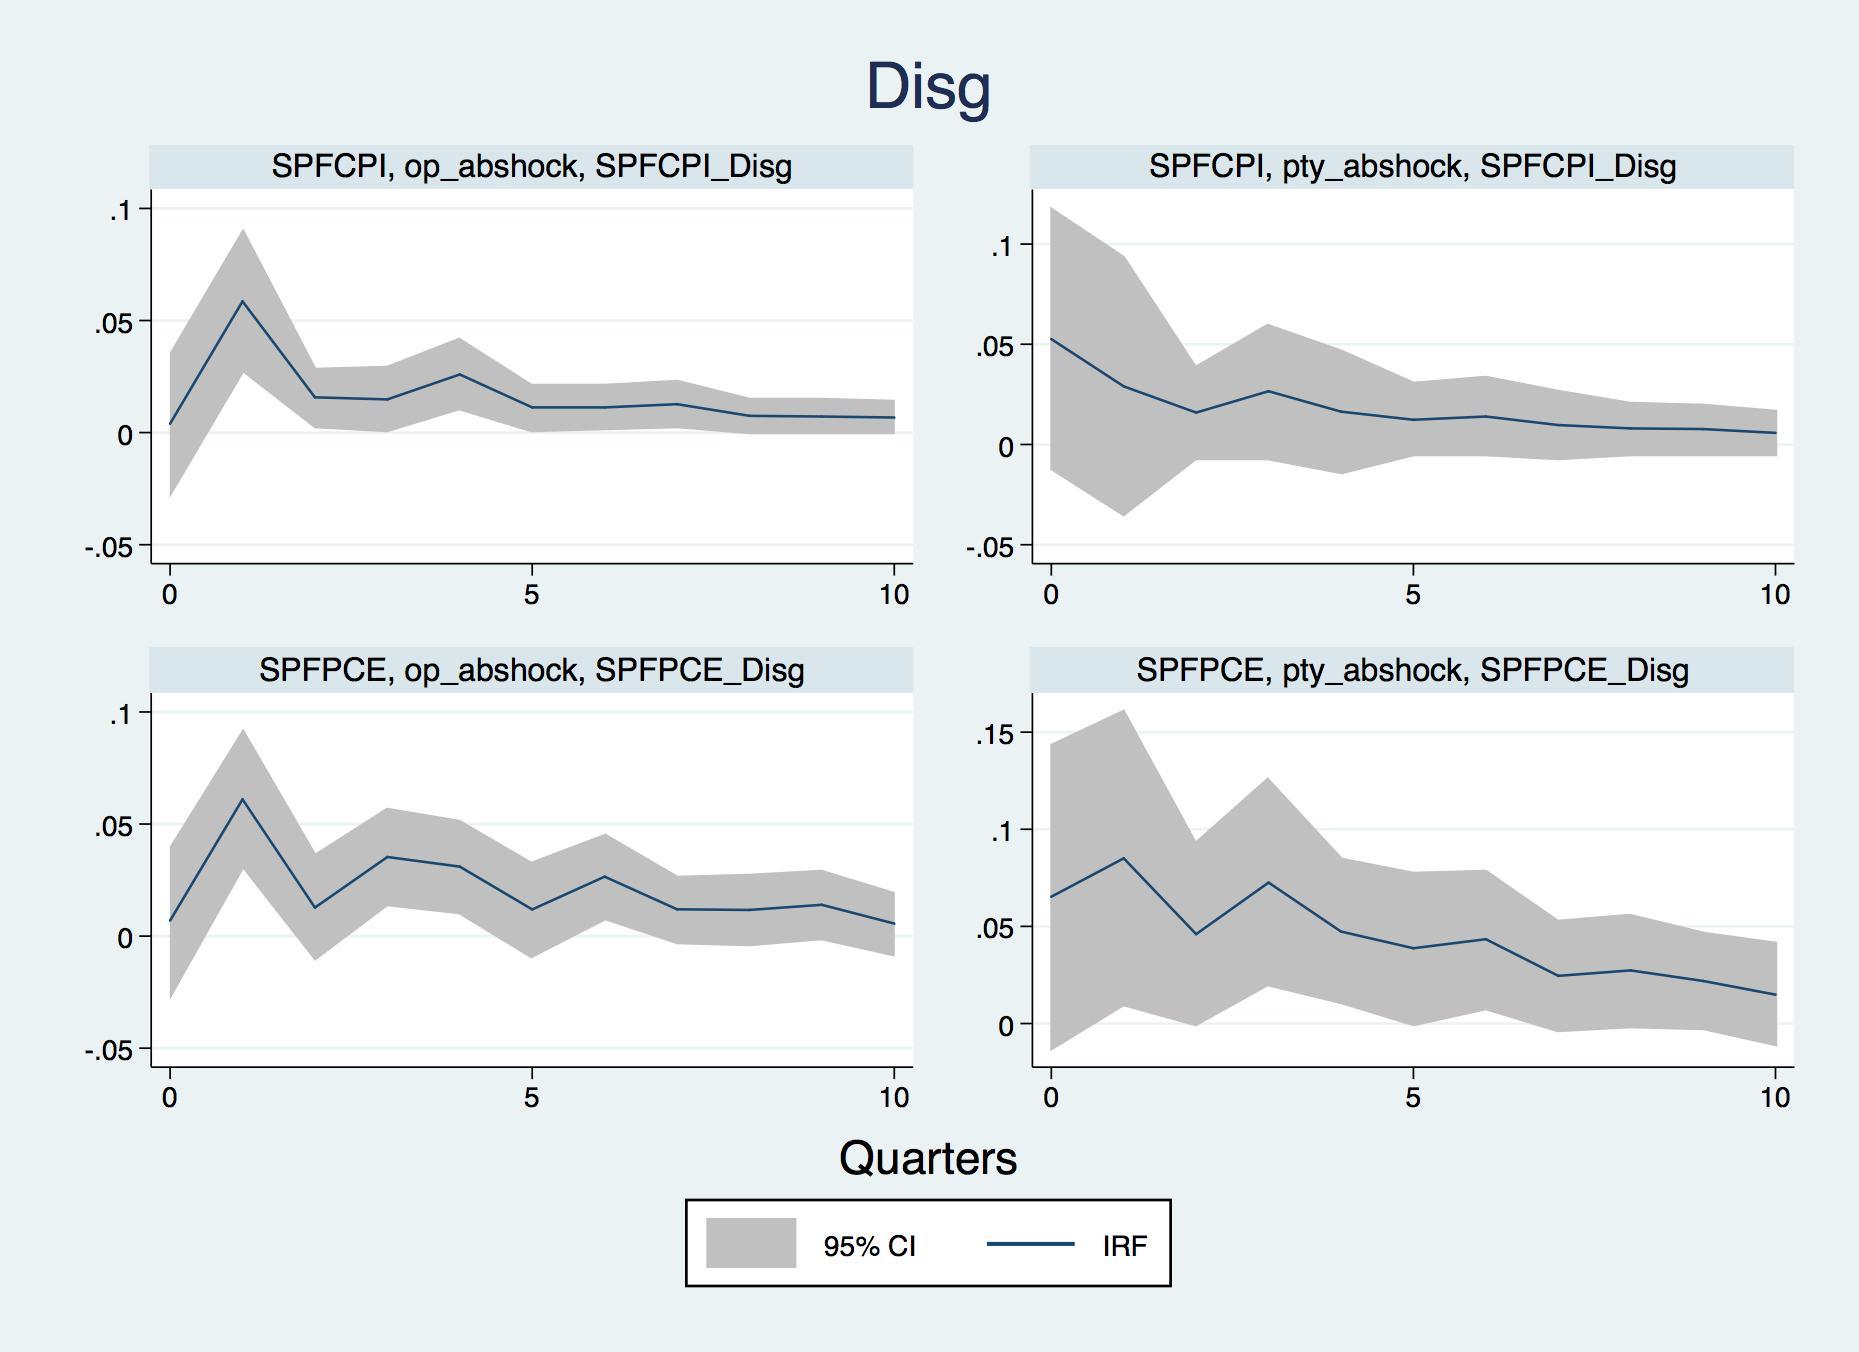
\includegraphics[width=6cm]{figures/SPFDisg_ab_ashocks_nmp.png} 
		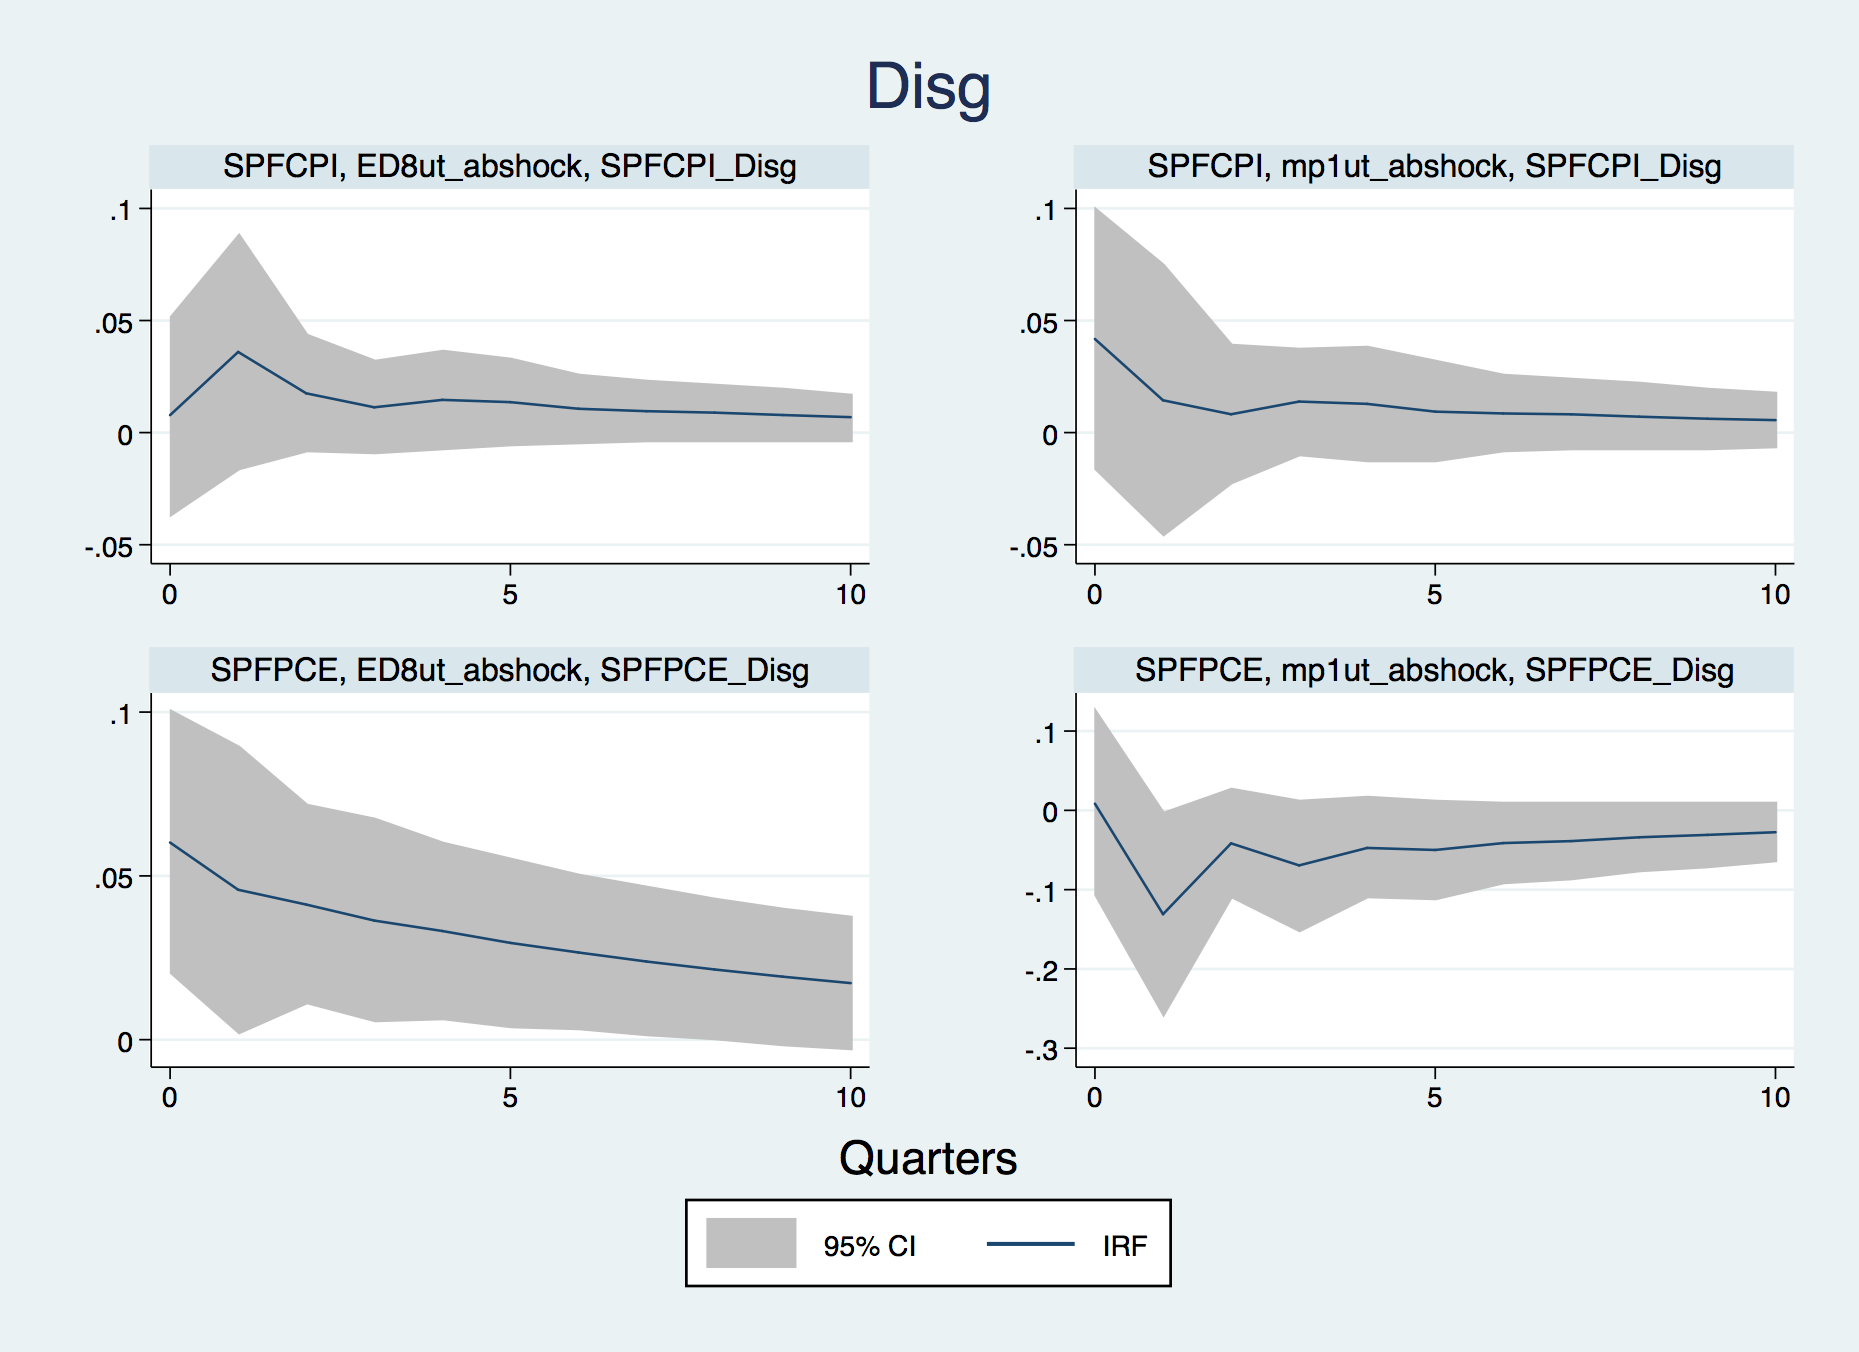
\includegraphics[width=6cm]{figures/SPFDisg_ab_ashocks.png} 
	\caption{ Replicating \cite{coibion2012can}: 1987-2007}
\end{figure}


\begin{figure}[h]\label{ReplicateCoibionpost2007}
	\centering
	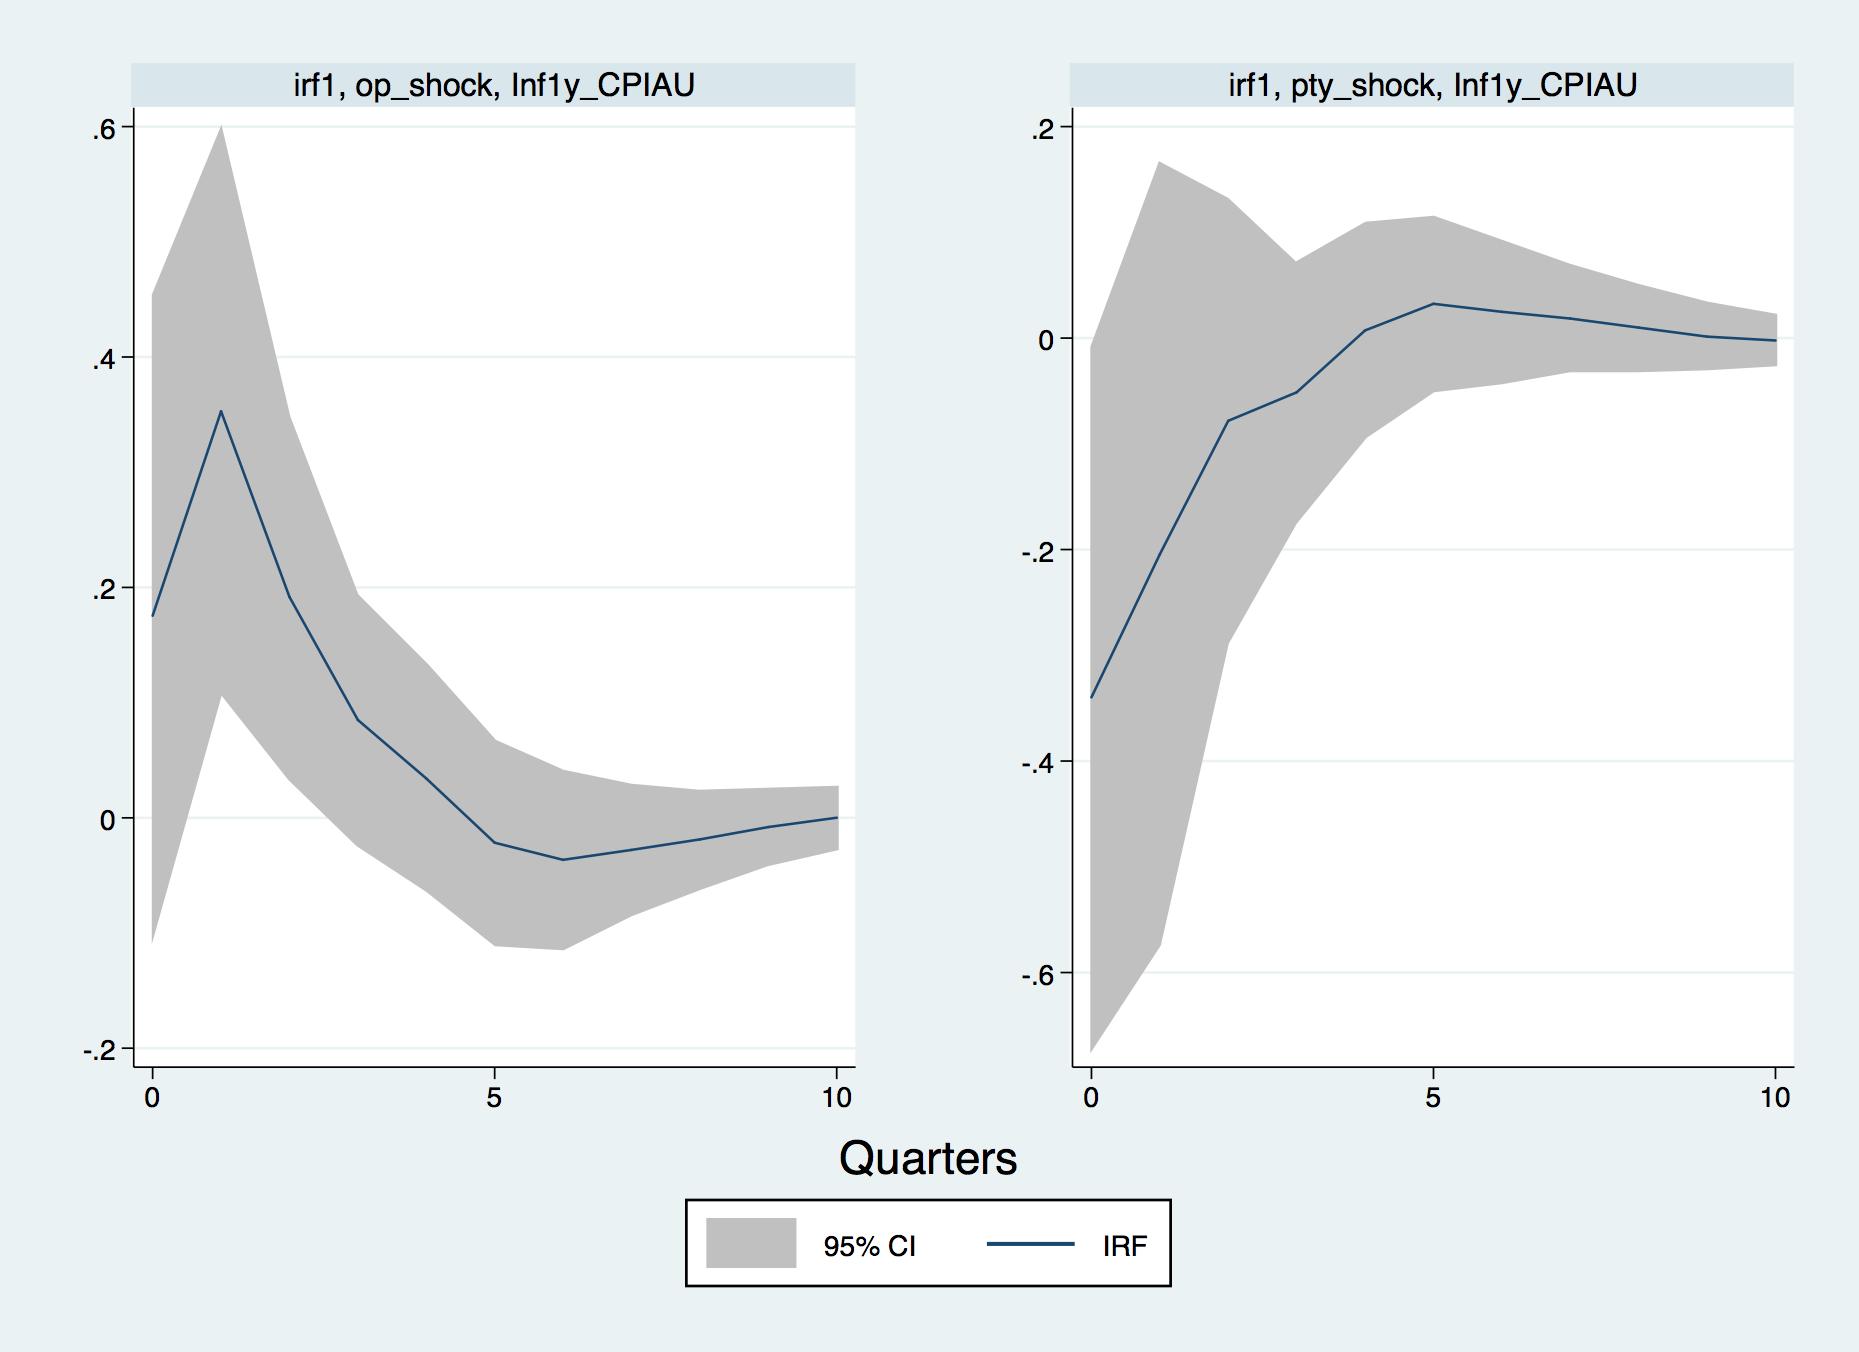
\includegraphics[width=6cm,height=2cm]{figures/CPIAU_ashocks_nmp_post2007.png}  
	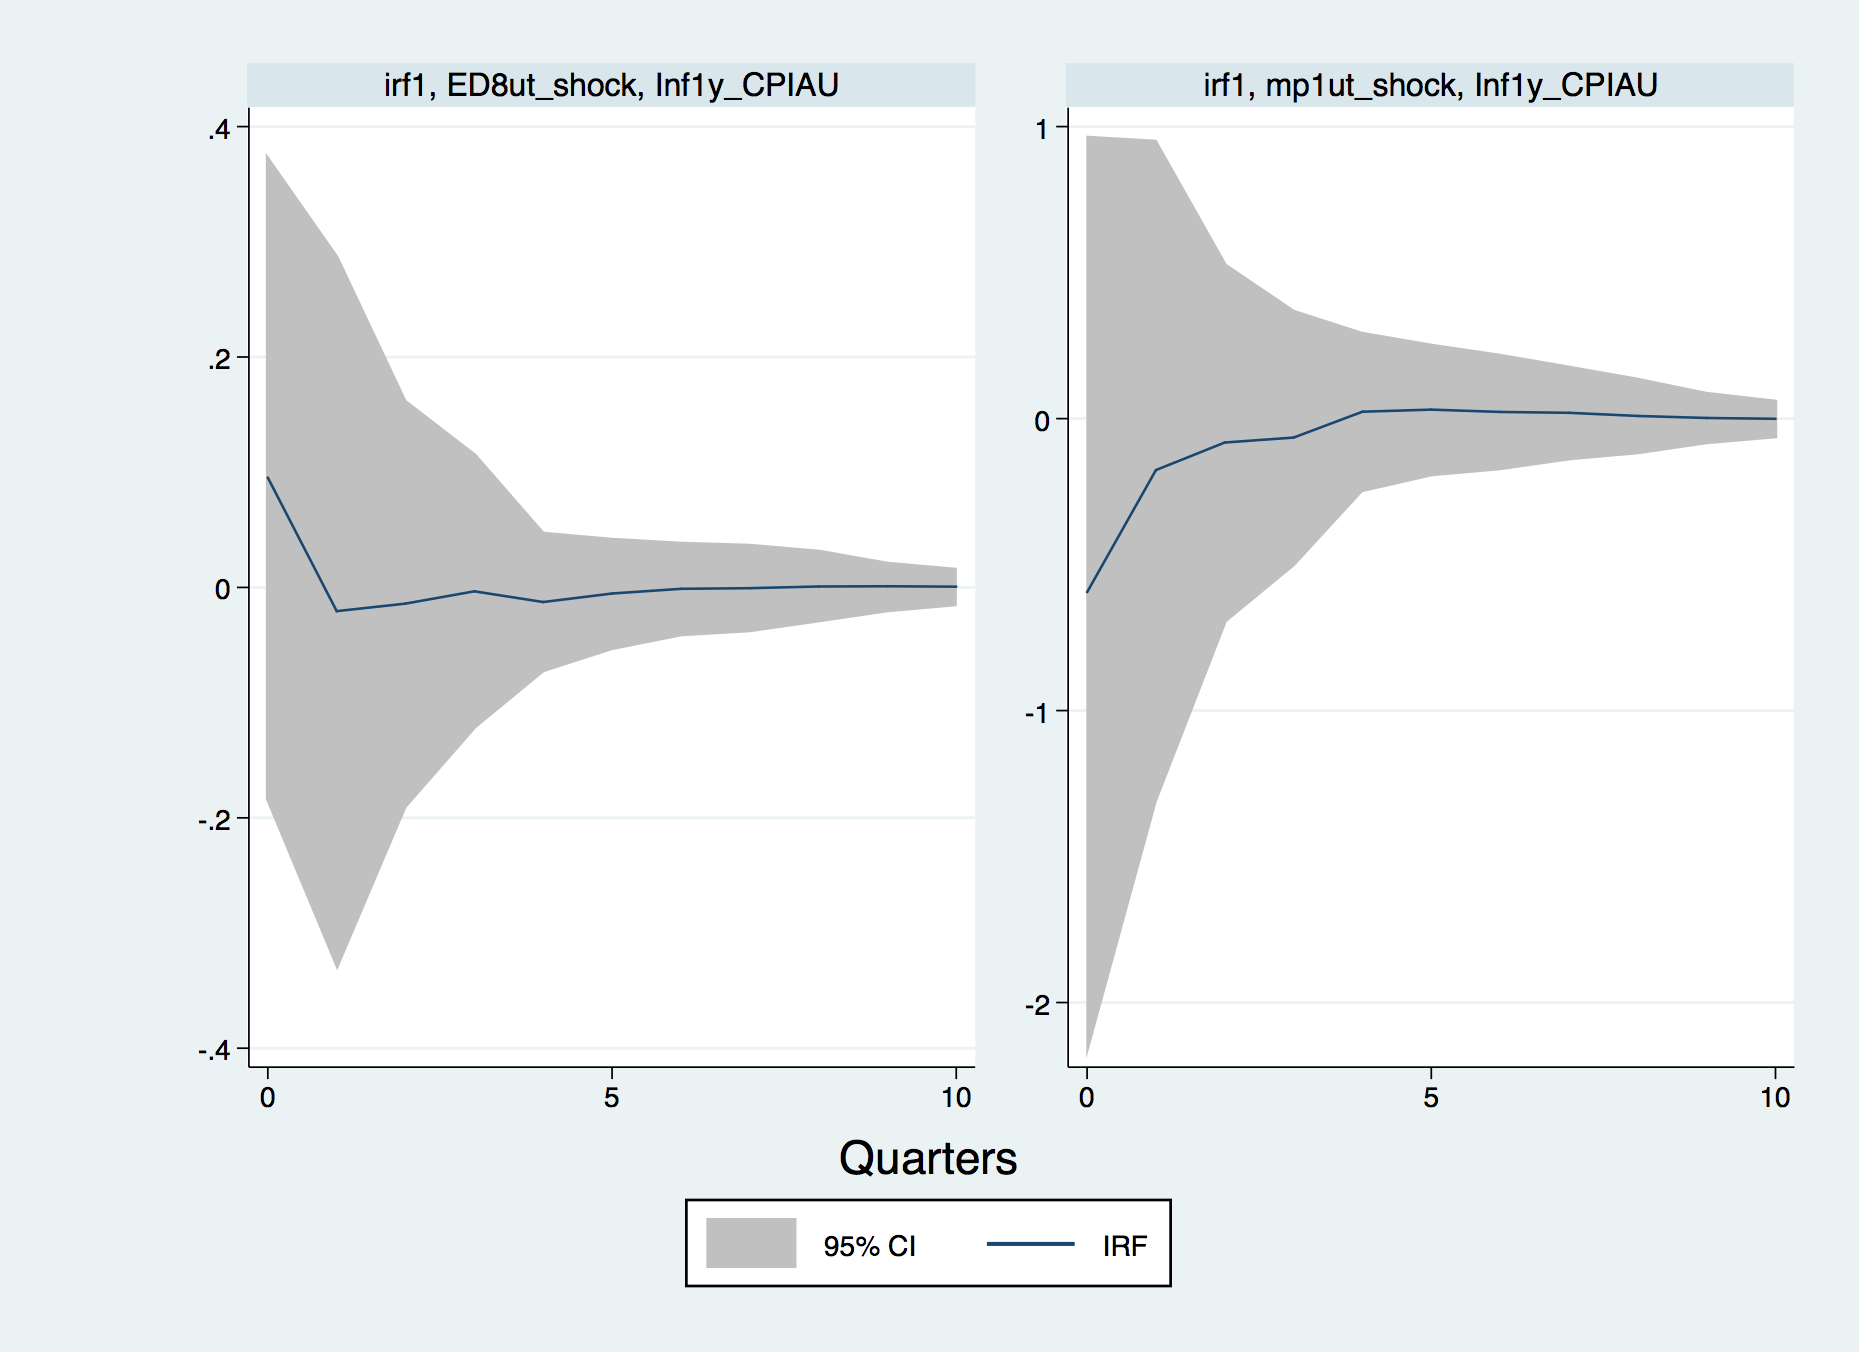
\includegraphics[width=6cm,height=2cm]{figures/CPIAU_ashocks_post2007.png} \\
	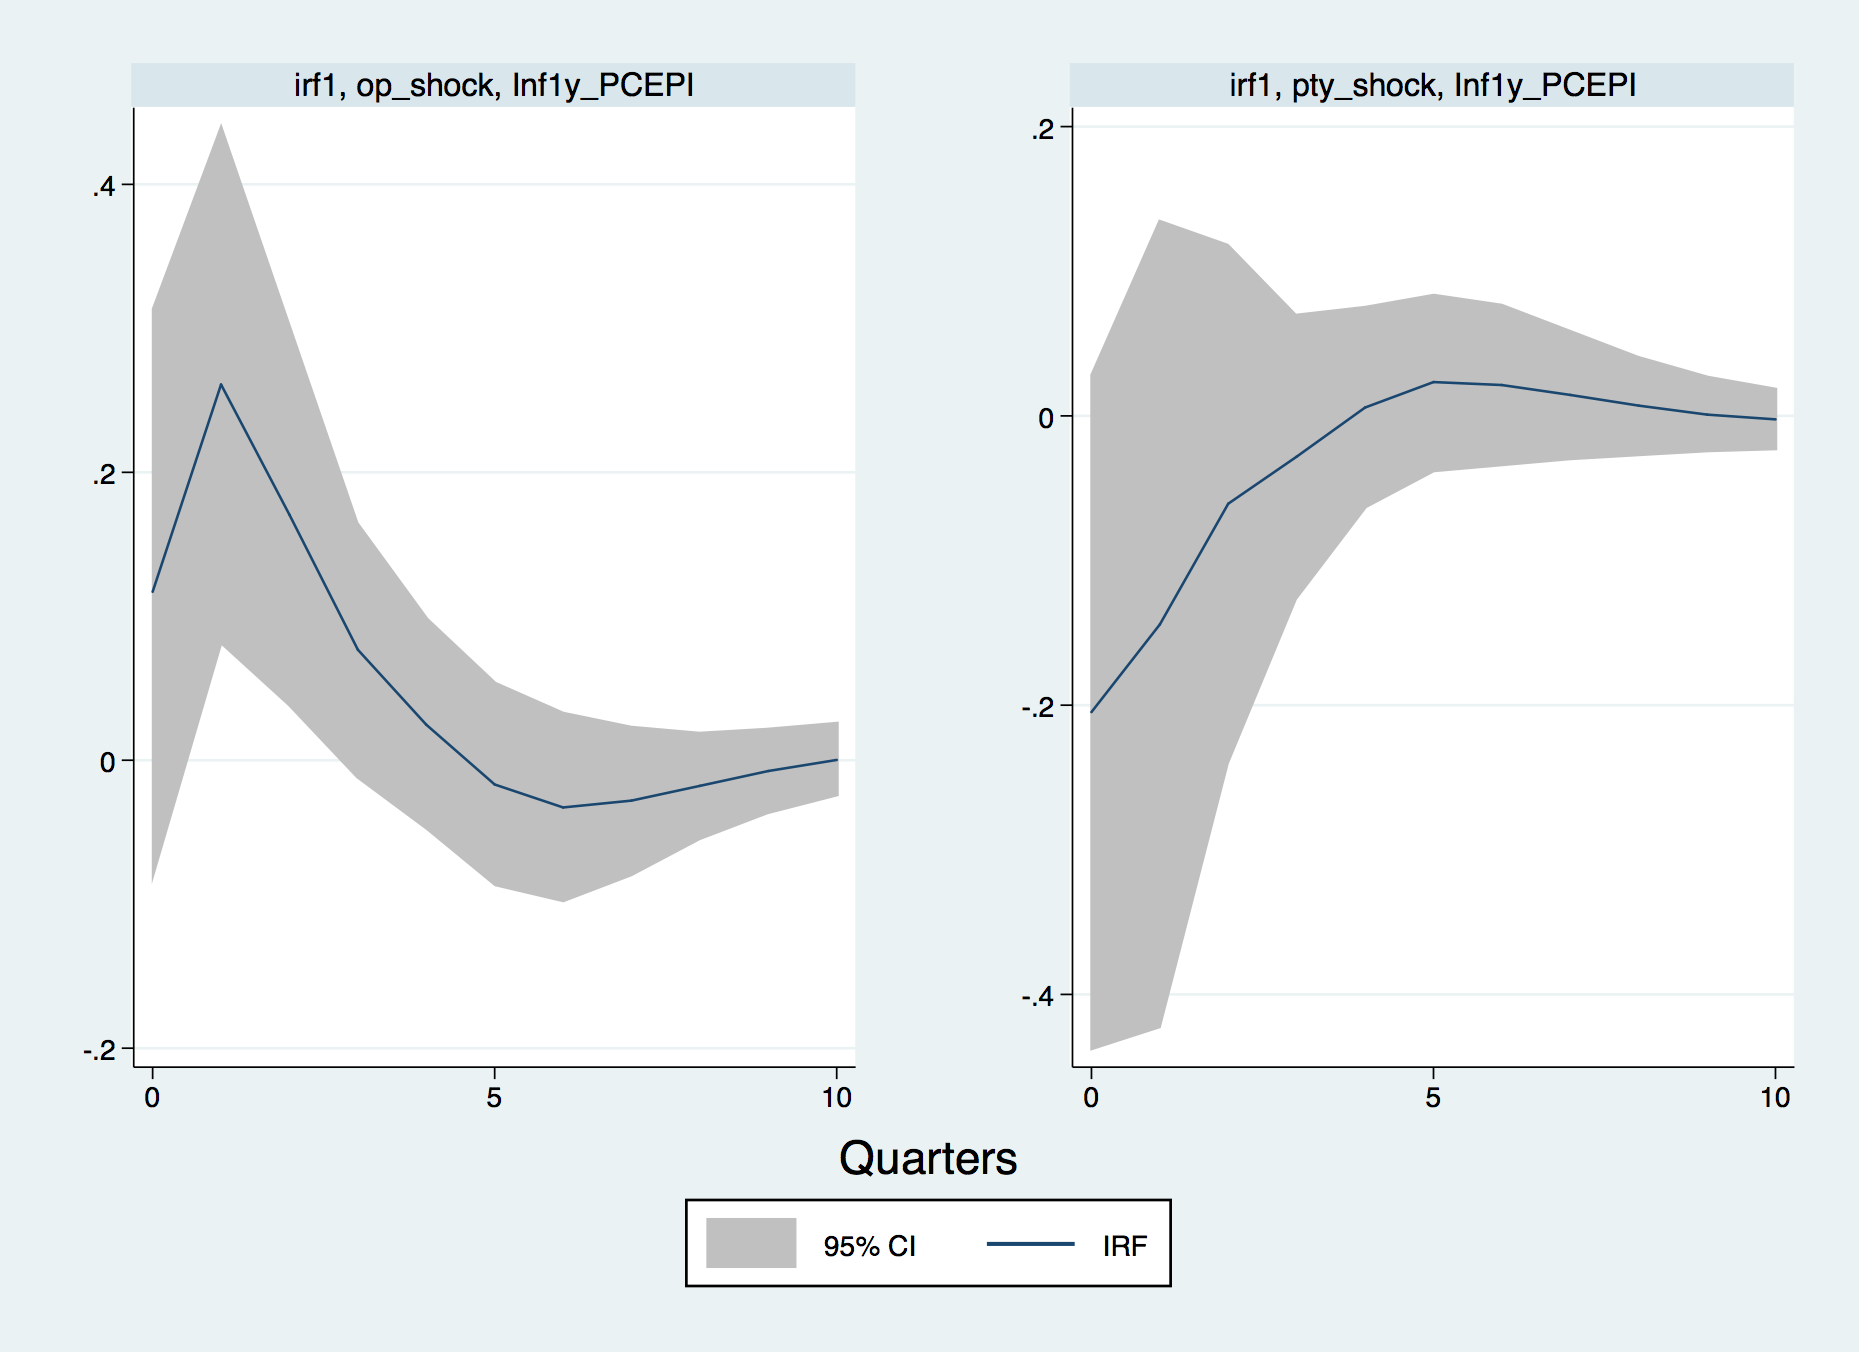
\includegraphics[width=6cm,height=2cm]{figures/PCEPI_ashocks_nmp_post2007.png} 
	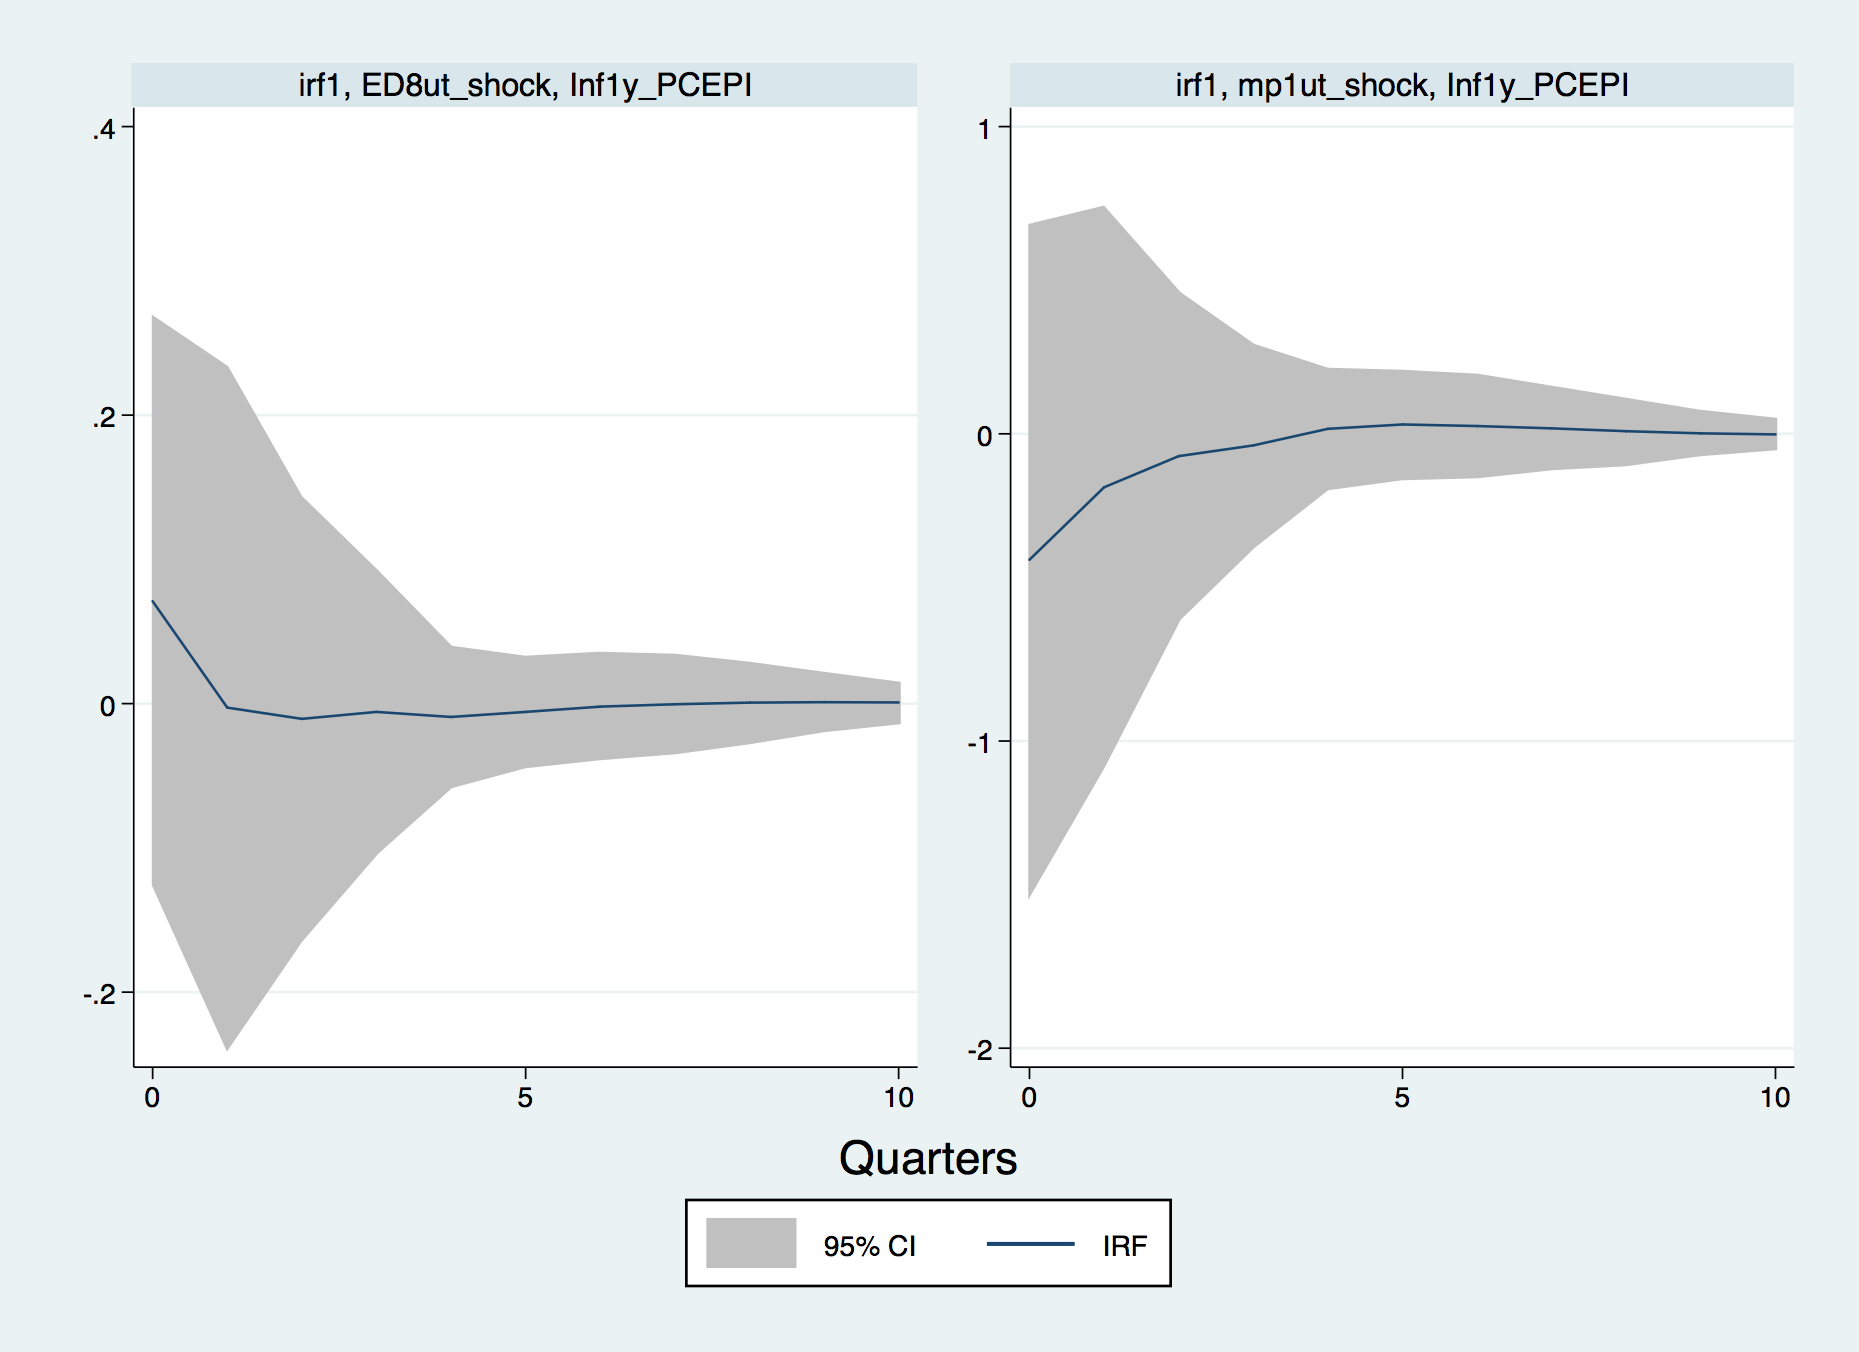
\includegraphics[width=6cm,height=2cm]{figures/PCEPI_ashocks_post2007.png}  \\
	\smallskip
	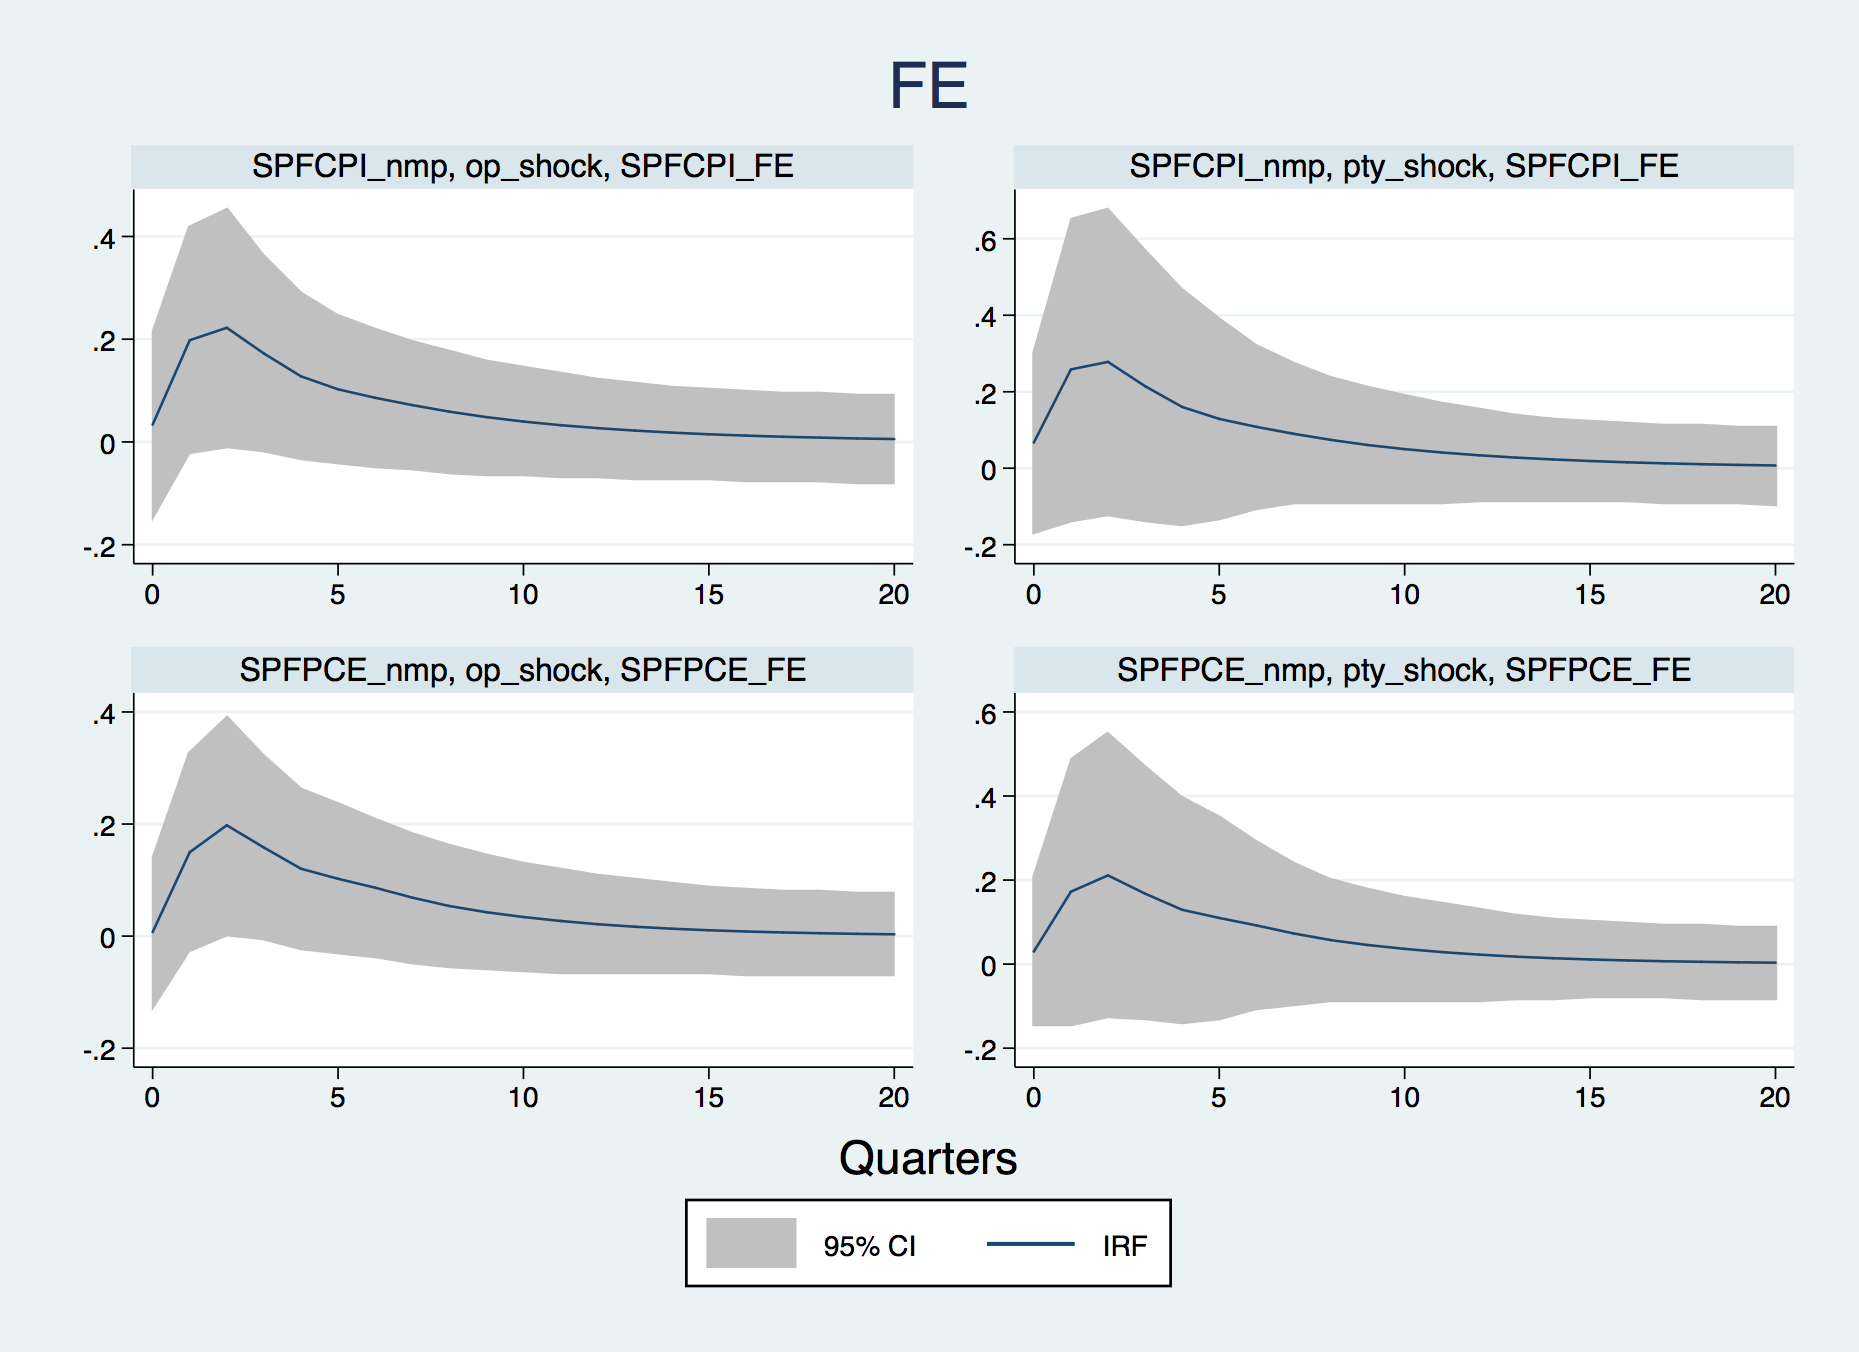
\includegraphics[width=6cm]{figures/SPFFE_ashocks_nmp_post2007.png} 
	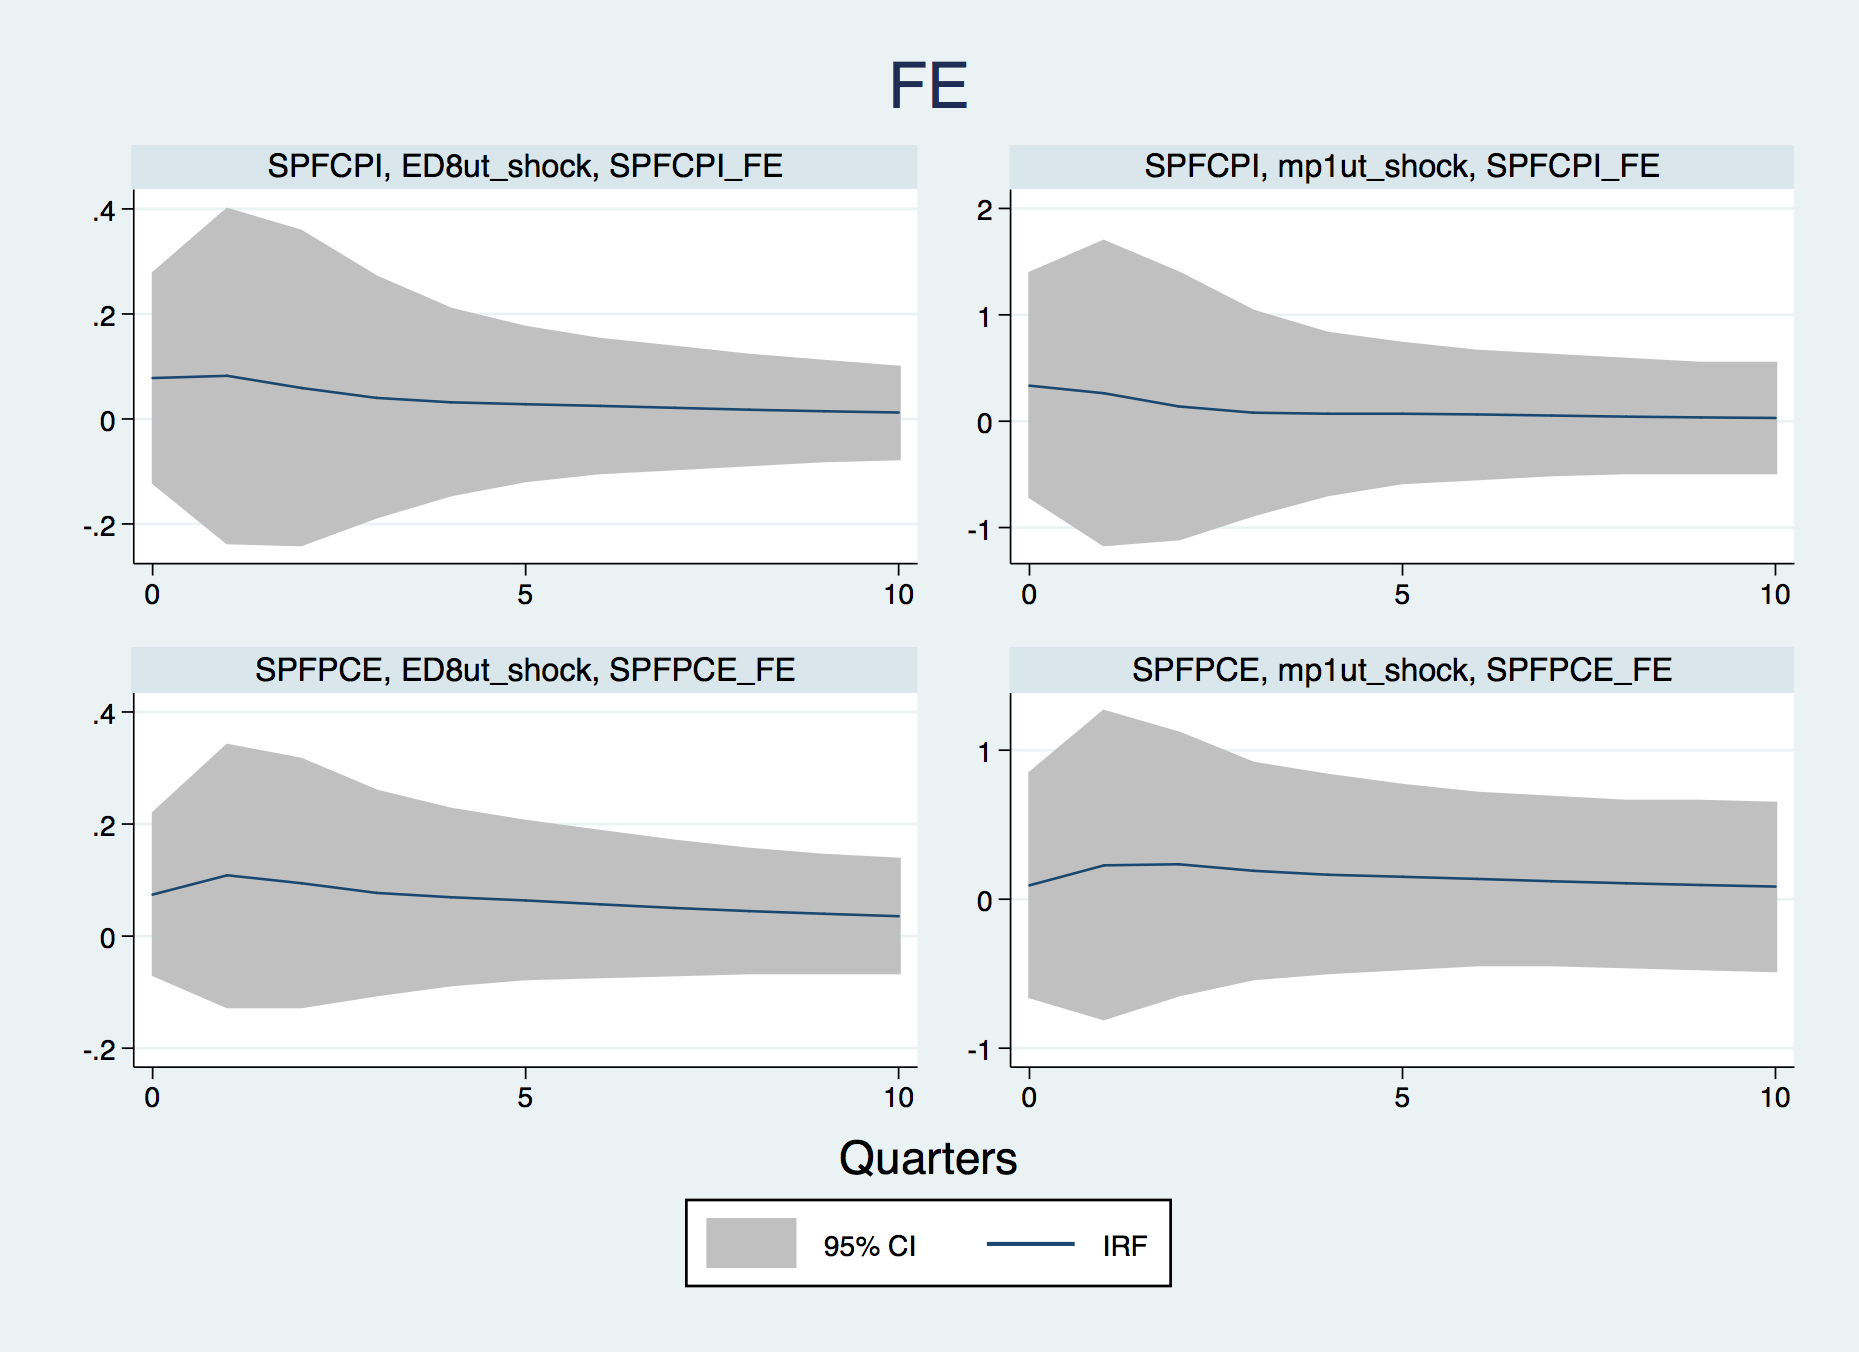
\includegraphics[width=6cm]{figures/SPFFE_ashocks_post2007.png} \\
	\smallskip
	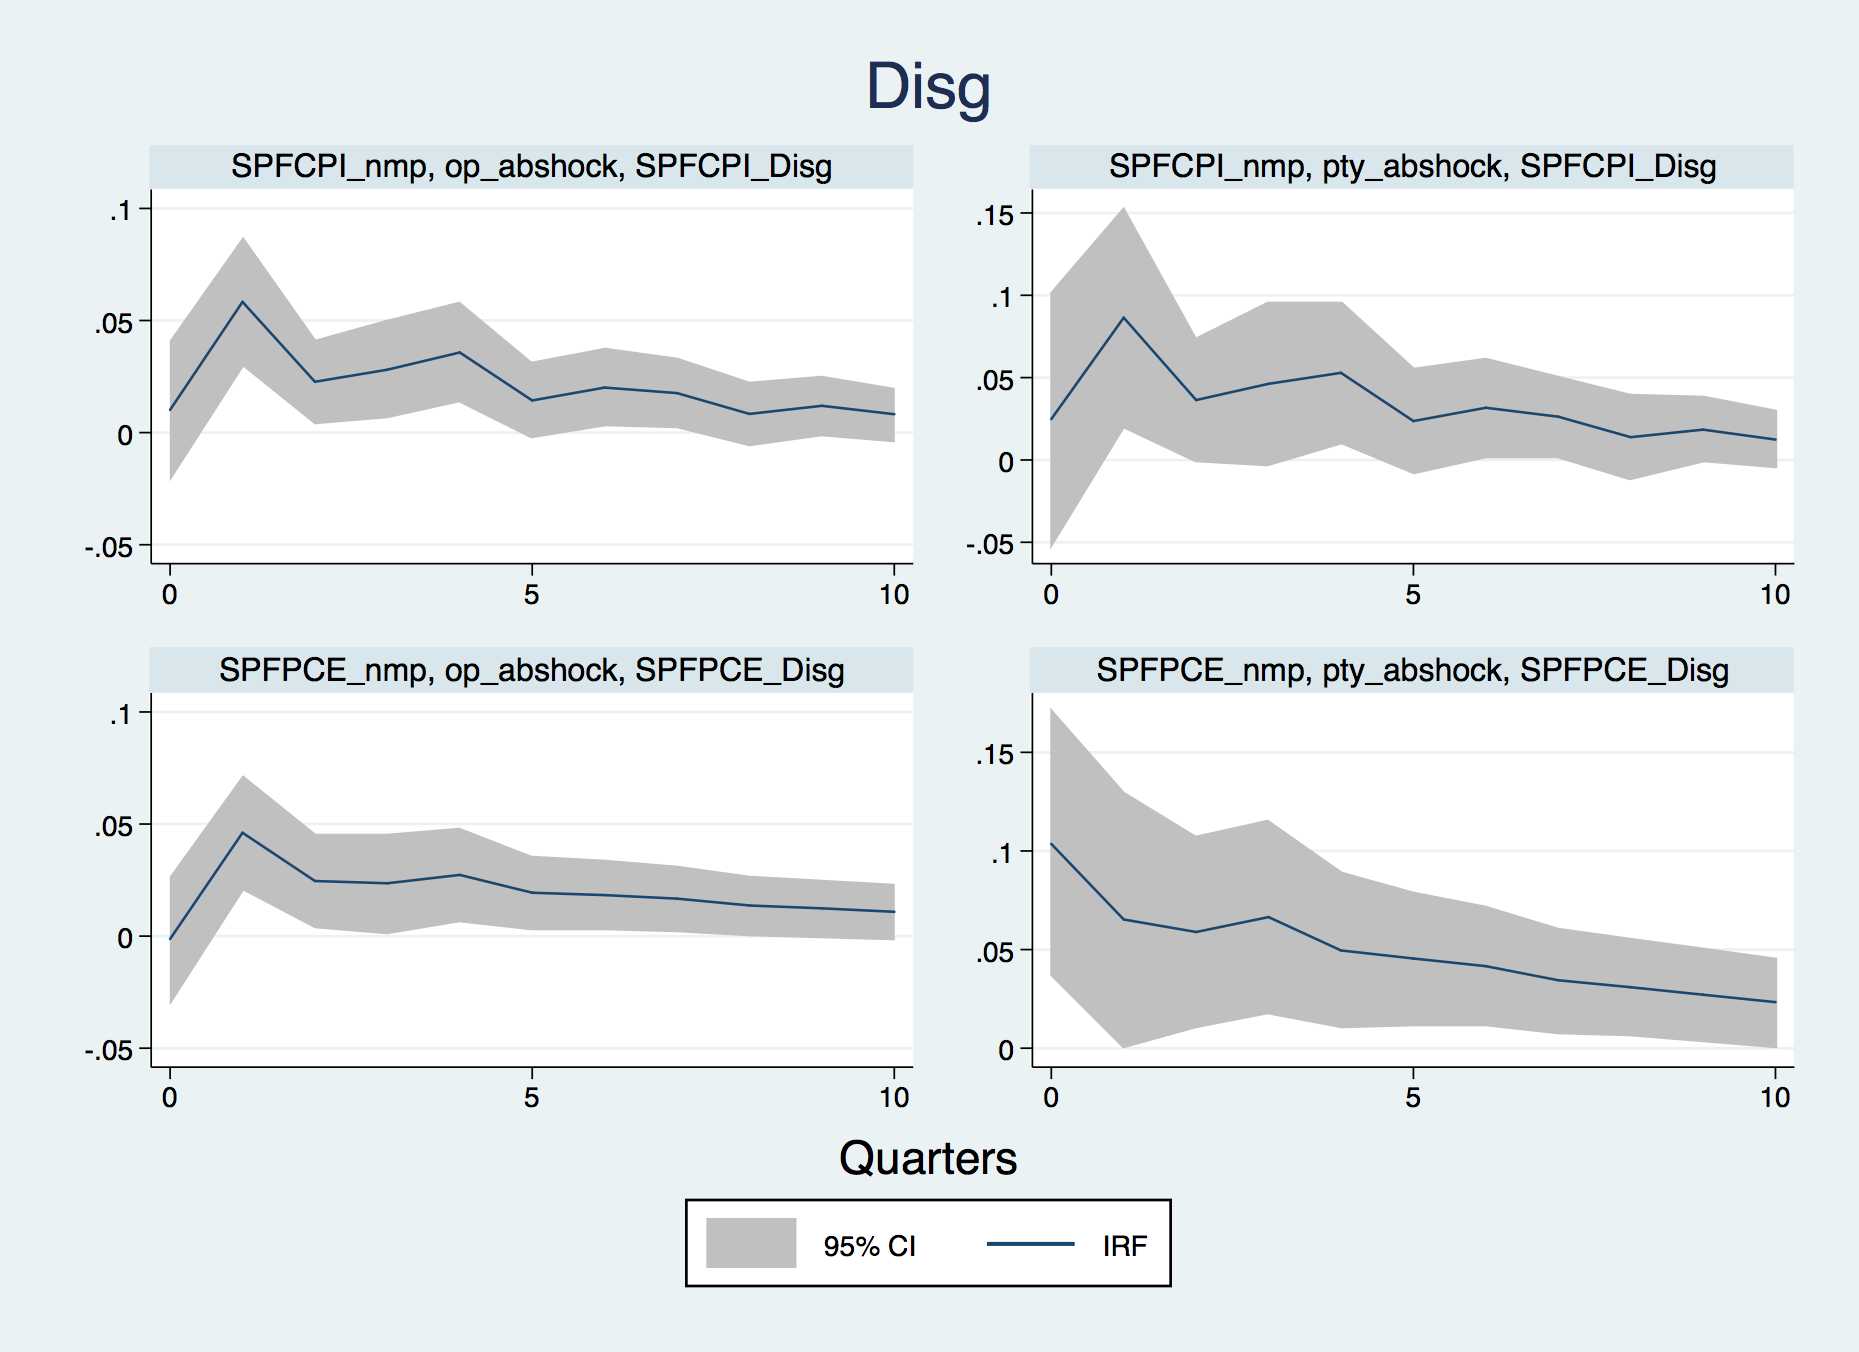
\includegraphics[width=6cm]{figures/SPFDisg_ab_ashocks_nmp_post2007.png} 
	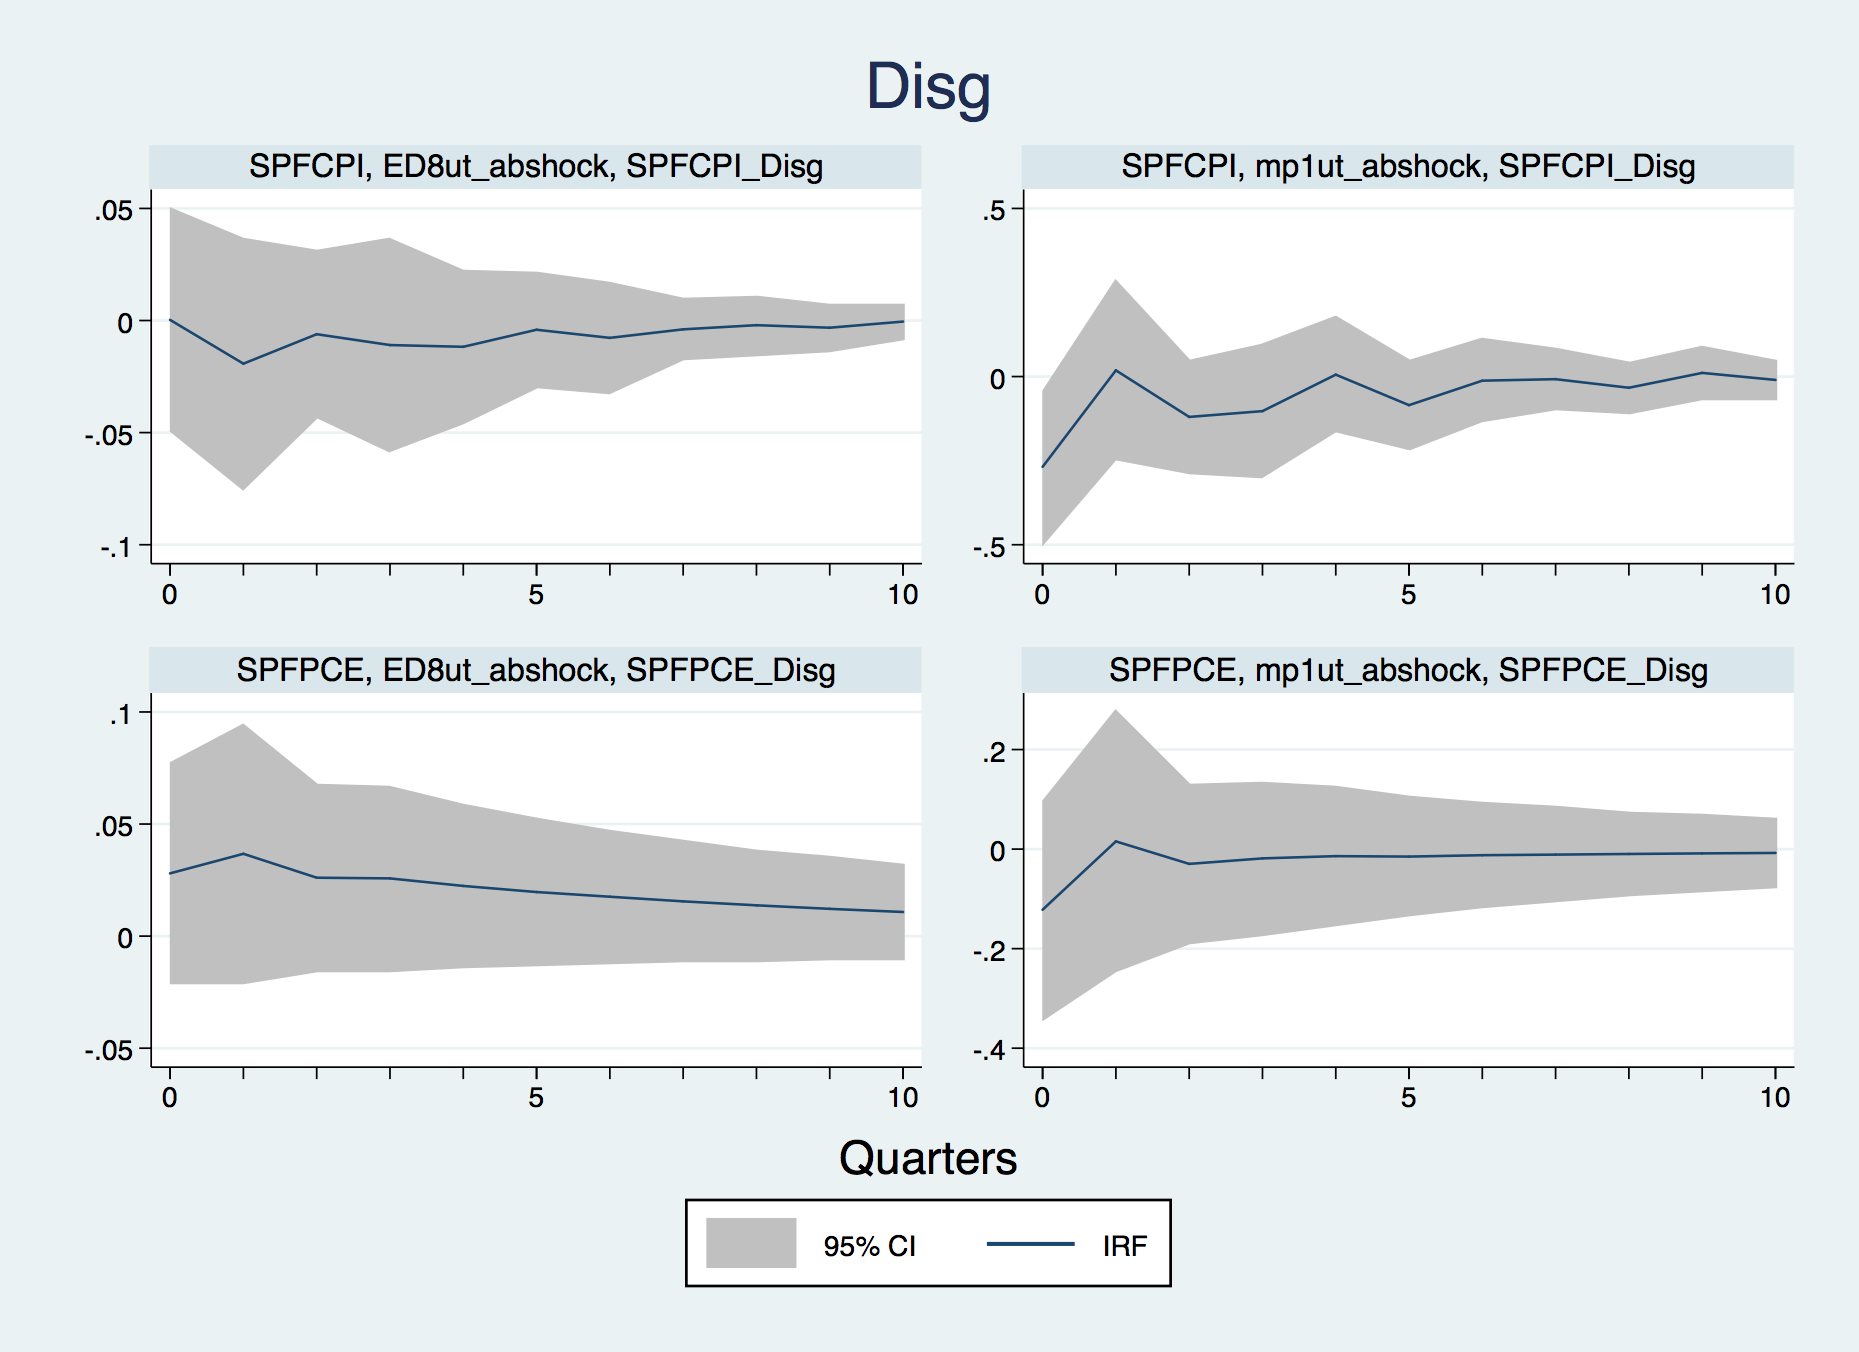
\includegraphics[width=6cm]{figures/SPFDisg_ab_ashocks_post2007.png} \\
	\smallskip 
		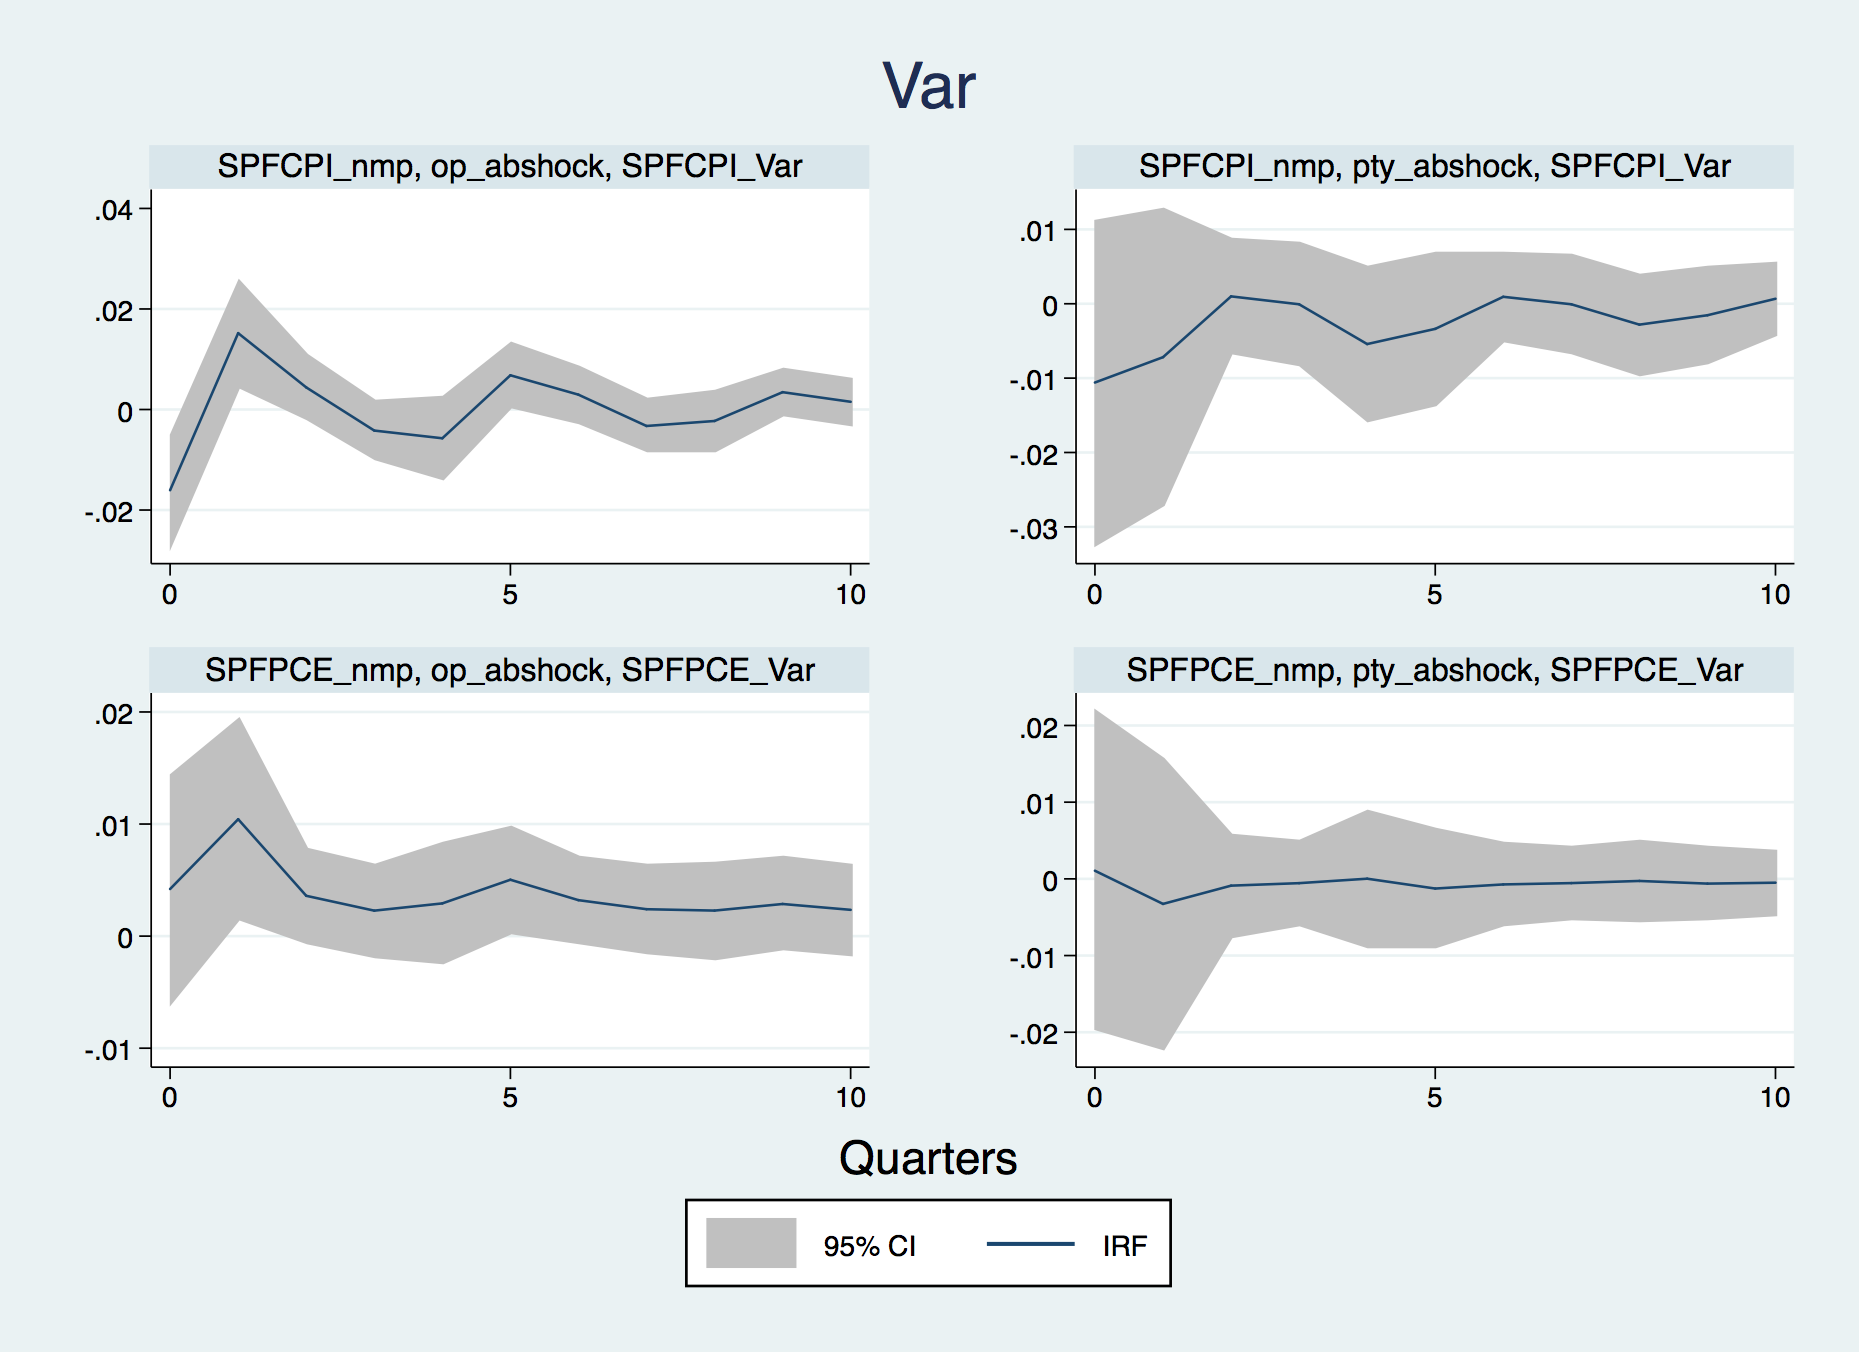
\includegraphics[width=6cm]{figures/SPFVar_ab_ashocks_nmp_post2007.png} 
	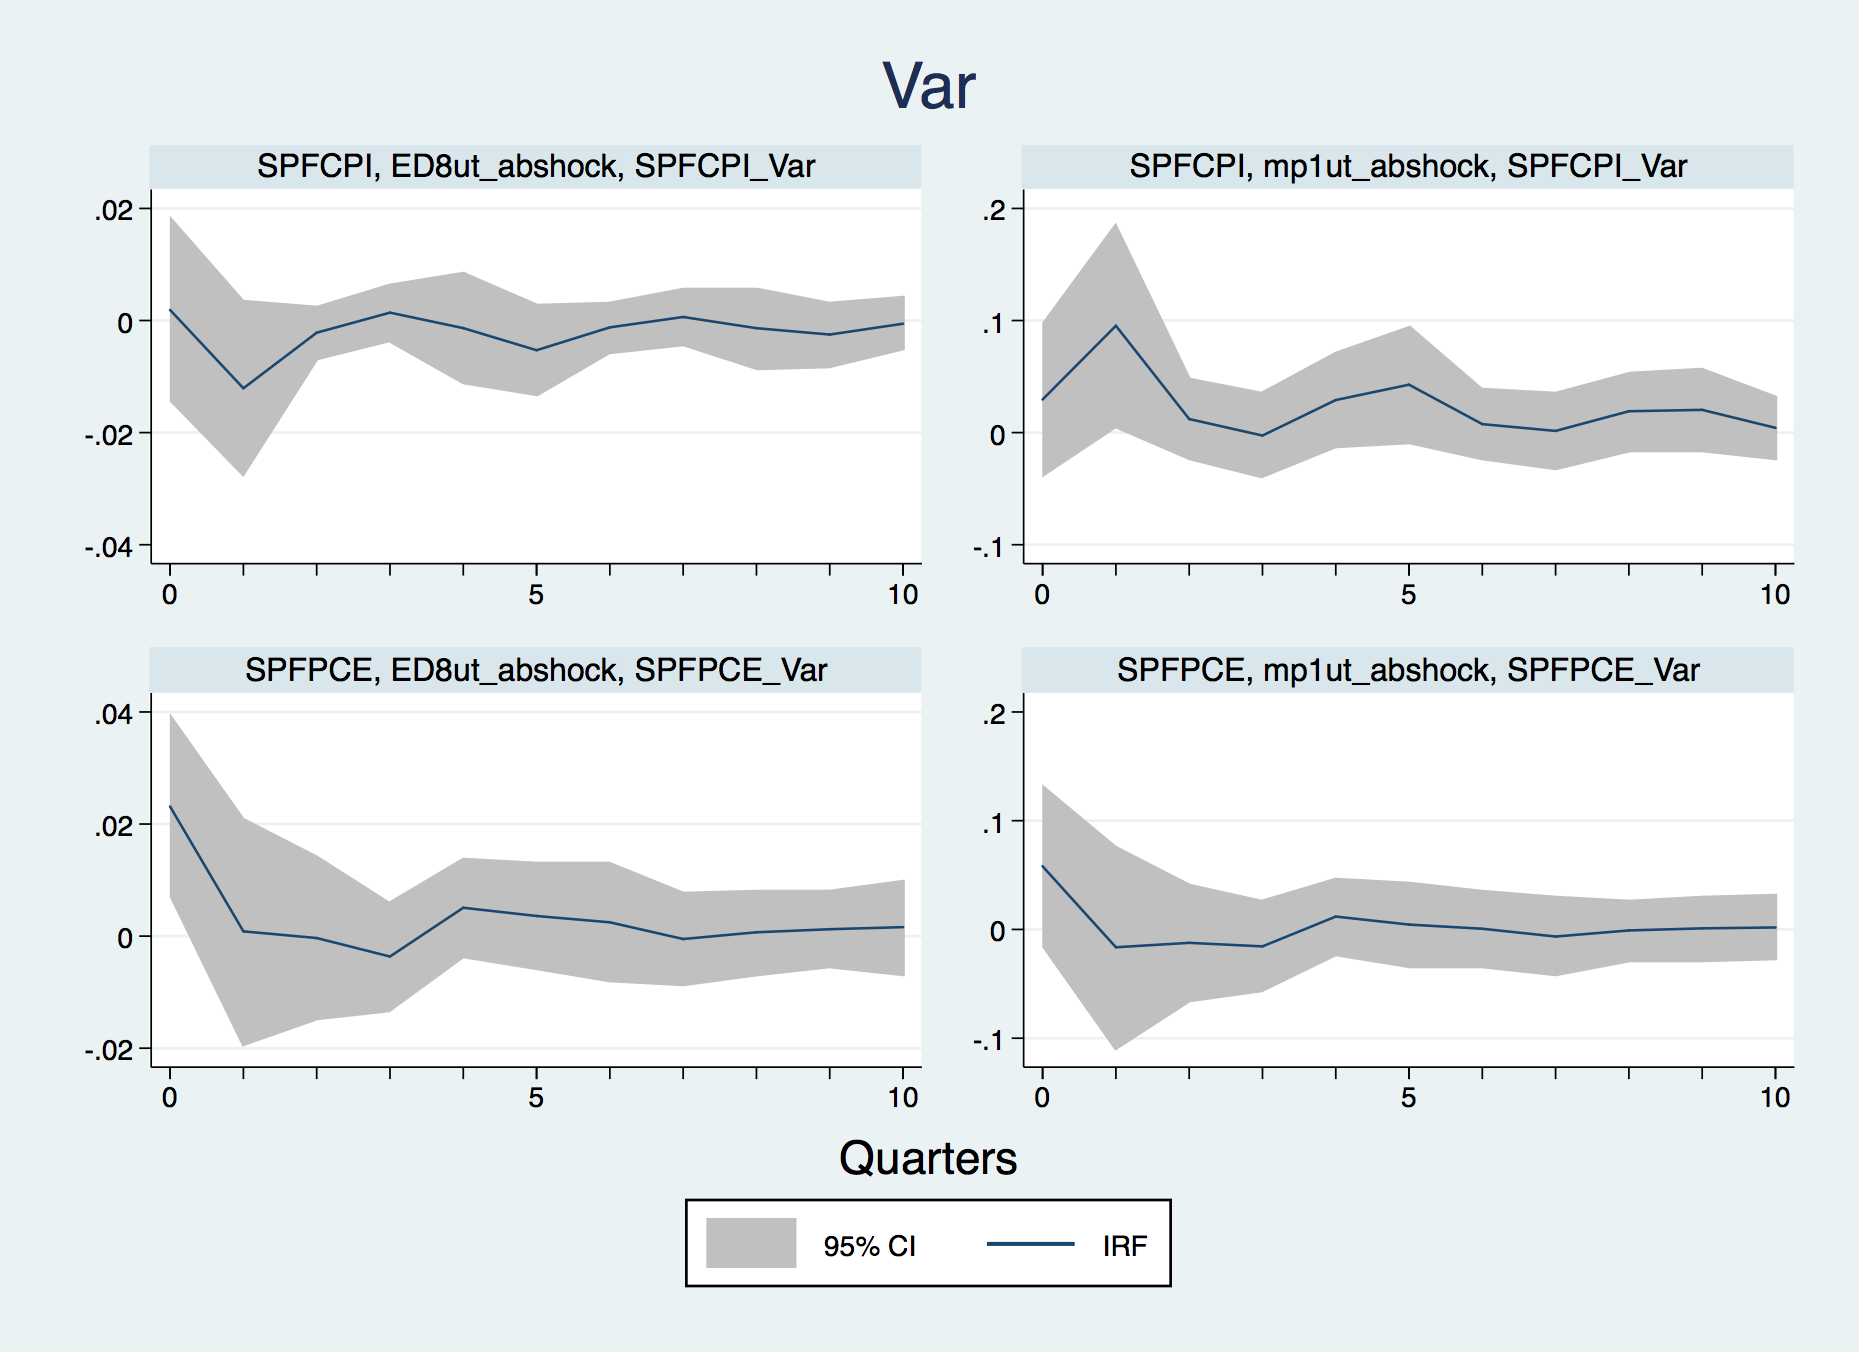
\includegraphics[width=6cm]{figures/SPFVar_ab_ashocks_post2007.png} 
	\caption{ Replicating \cite{coibion2012can}: 2008-2019}
\end{figure}



\subsubsection{Additional Evidence from Uncertainty}

\subsection{Evidence from Households}

\section{Conclusion}


\bibliographystyle{apalike}
\bibliography{TestingExpectationTheories}

\end{document}
